%\vspace{-.2in}
\section{Experiments}\label{sec:expts}~
In the following, we evaluate Python implementations of a number of algorithms, focusing our contribution, the symmetrized MH algorithm (algorithm~\ref{alg:MH_improved}), and as well as the \naive\ MH algorithm (algorithm~\ref{alg:MH_naive}).
%, which we plot \boqian{as yellow twodashed  lines}), 
%, plotted \sout{as dashed red lines}\boqian{as solid blue lines}
We evaluate different variants of these algorithms, corresponding to different uniformizing Poisson rates. % (i.e.\ different choices of $\kappa$, see section~\ref{sec:comments}). 
For \naive\ MH, we set $\Omega(\theta) = \kappa \max_s A_s(\theta) $ with $\kappa$  equal to $1.5, 2$ and $3$ (here $\kappa$ must be greater than $1$), 
%represented in our plots with circles, \sout{triangles} \boqian{square} and \sout{square} \boqian{triangles} symbols. 
while for symmetrized MH, where the uniformizing rate depends on both the current and proposed parameters, we consider the settings:
 $\Omega(\theta, \vartheta) = \kappa (\max A(\theta) + \max A(\vartheta))$ 
 ($\kappa = 1$ and $1.5$), and 
 %, plotted with \sout{triangles} \boqian{square} and \sout{square} \boqian{triangles}), and 
$\Omega(\theta, \vartheta) = 1.5 \max(\max A(\theta), \max A(\vartheta))$.
%($\kappa=1.5$, plotted with {circles}).  
We evaluate two other baselines: Gibbs sampling (Algorithm~\ref{alg:MJP_gibbs}), %plotted \sout{in blue} \boqian{as red long dashed lines} ), 
and particle MCMC~\citep[][see also section~\ref{sec:pmcmc} in the appendix]{Andrieu10}. 
%plotted \sout{in black} \boqian{as black dashed lines}. 
Gibbs sampling involves a uniformization step to update the MJP trajectory (step 1 in algorithm~\ref{alg:MJP_gibbs}), for which we use $\Omega(\theta,\vartheta) = \kappa \max_s A_s(\theta)$ for $\kappa=1.5,2,3$. 
%plotted with circles, \sout{triangles} \boqian{square} and \sout{square} \boqian{triangles}.  
Unless specified, our results were obtained from $100$ independent MCMC runs, each of $10000$ iterations.
We found particle MCMC to be more computationally intensive, and limited each run to $3000$ iterations, the number of particles being $5, 10$ and $20$.%(plotted with circles, \sout{triangles} \boqian{square} and \sout{square} \boqian{triangles}). 

% We also considered exploiting gradient information of the target distribution to apply Hamiltonian Monte Carlo (HMC)~\cite{Neal2010}. In particular, the forward pass of FFBS allows us to also calculate the gradient of the log-probability with respect to the MJP parameters. We can exploit this information for more directed explorations of parameter space than a random-walk algorithm. Of course, this comes at a higher computational cost. We evaluate HMC with the number of leapfrog steps taking values in $1, 3, 5$ or $10$, and the leapfrog stepsize taking values in $0.02, 0.05$ and $0.1$. 

For each run of each MCMC algorithm, we calculated the effective sample size (ESS) of the posterior samples of the MJP parameters using the R package \texttt{rcoda}~\citep{Rcoda2006}. 
This estimates the number of independent samples returned by the MCMC algorithm, and dividing this by the runtime of a simulation gives the ESS per unit time (ESS/sec). 
We used this to compare different samplers and different parameter settings.

\subsection{A simple synthetic MJP}
\begin{wrapfigure}{r}{.4\textwidth}
    \vspace{-.3in}
  \begin{minipage}[!hp]{.05\linewidth}
    \hspace{.1in}
  \end{minipage}
  \begin{minipage}[!hp]{.9\linewidth}
  \centering
    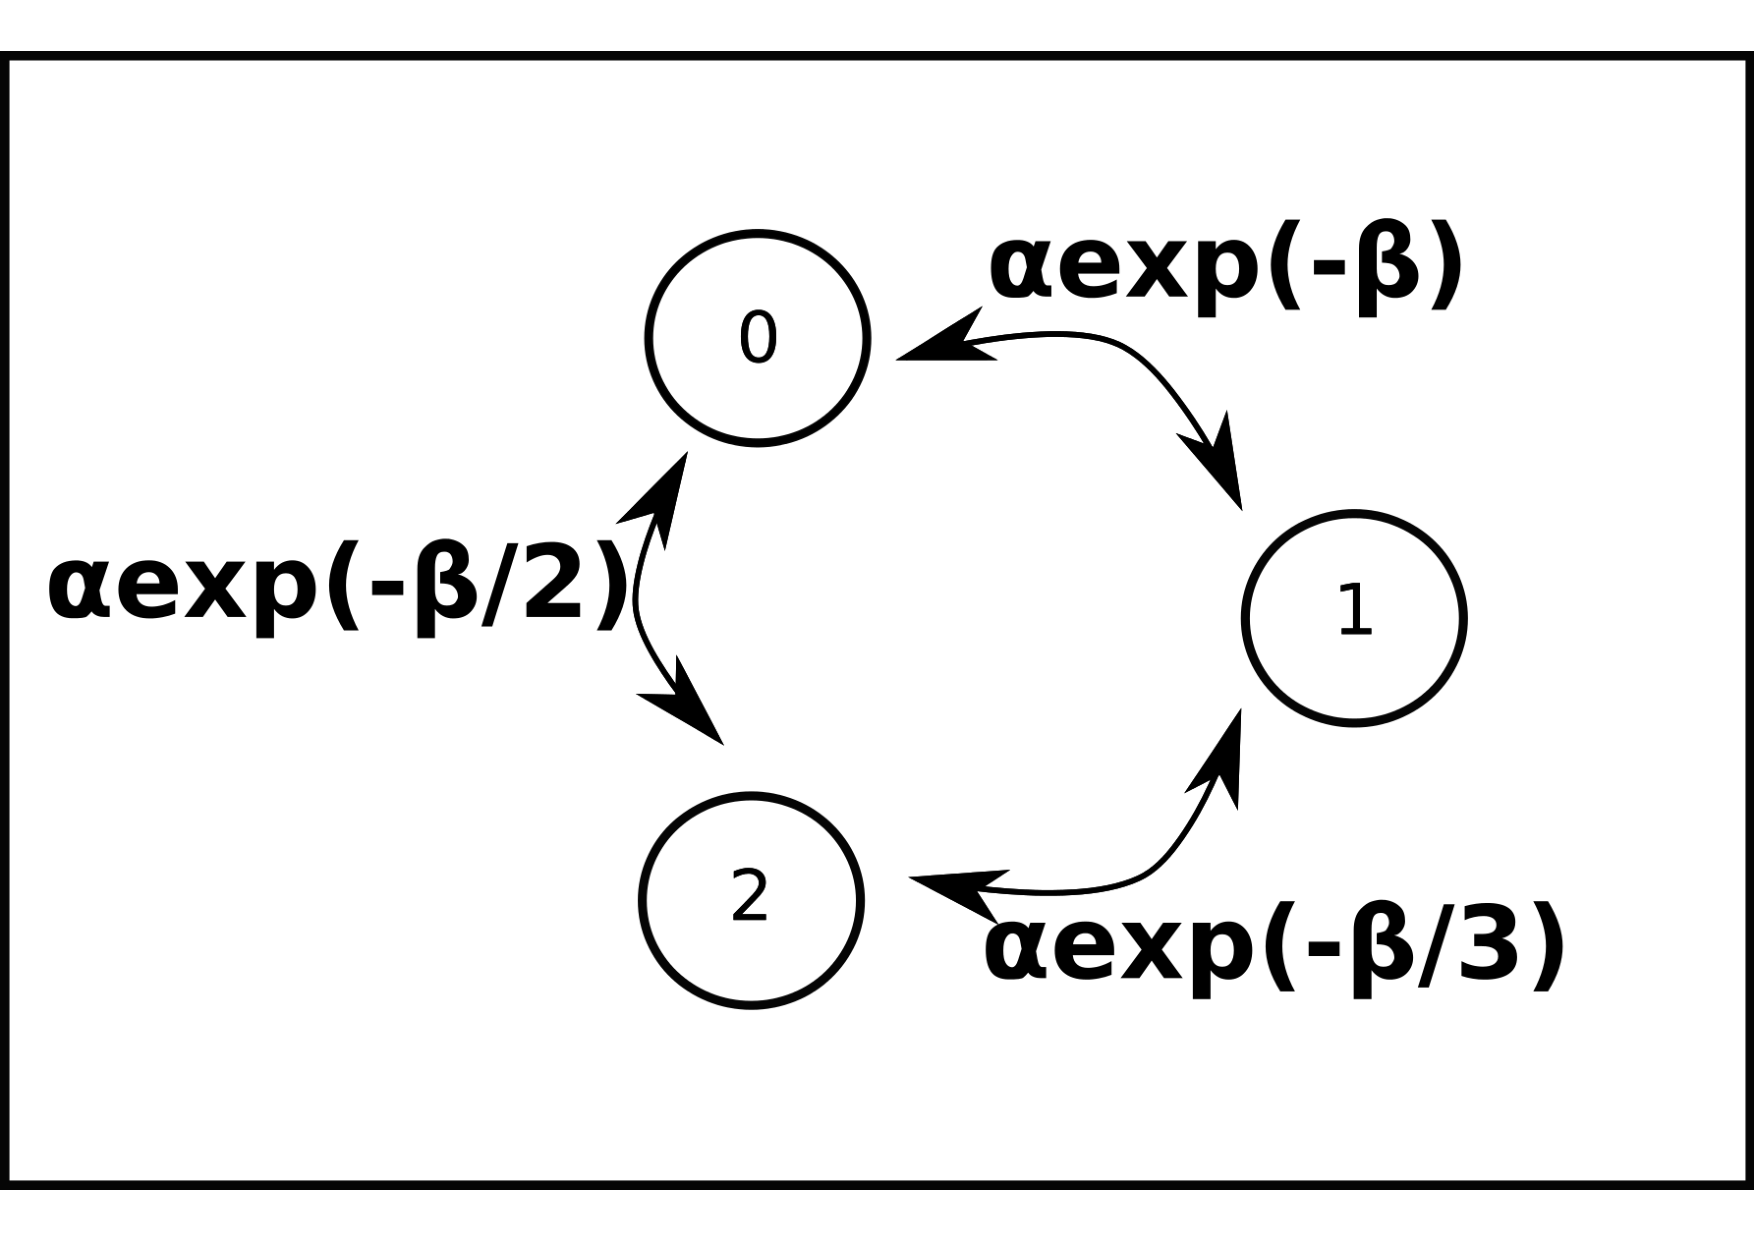
\includegraphics [width=\textwidth, angle=0]{figs/exp_model.pdf}
    \caption{A 3-state MJP with exponentially decaying rates}
    \label{fig:exp_model}
      \end{minipage}
%    \vspace{-.1in}
  \end{wrapfigure}
  Consider an MJP with a uniform distribution over states at time $0$, and with transitions between states $i$ and $j$ having rate $\alpha \exp(-\beta/(i+j))$, for two parameters $(\alpha,\beta) \defeq \theta$. 
We consider three settings: $3$ states (figure~\ref{fig:exp_model}), $5$ states, and $10$ states.
We place Gamma$(\alpha_0,\alpha_1)$, and Gamma$(\beta_0, \beta_1)$ priors on the parameters $\alpha$ and $\beta$, with $(\alpha_0,\alpha_1,\beta_0,\beta_1)$ having values $(3,2,5,2)$ respectively. 
For each run, we draw random parameters from the prior to construct a transition matrix $A$, and simulate an MJP trajectory.
We simulate observations uniformly at integer values on the time interval $[0, 20]$. 
Each observation is Gaussian distributed with mean equal to the state at that time, and variance equal to $1$.  
For the MH proposal, we used a lognormal distribution centered at the current parameter value, with variance $\sigma^2$ whose effect we study.  
% \noindent Assume: $S = [S_0,S_1, ...,S_N] \;, T = [t_0(t_{start}), t_1,...,t_N, t_{N+1}(t_{end})]$, and y as observations.\\
% We consider a specific structure of rate matrix $A$. $A_{ij} = \alpha f_{ij}(\beta), \; i \neq j$. $A_{ii} = -\sum_{j \neq i} A_{ij}$. $0 \leq f_{ij} \leq 1$. Denote $F_i(\beta) = \sum_{j \neq i} f_{ij}(\beta)$.\\
% \begin{align*}
% P(s_0, S, T | \alpha, \beta) &= \pi_0(s_0)\prod_{i = 1}^N A_{S_{i - 1}S_i} \exp(- \int_{t_{start}}^{t_{end}} |A_{S(t)}| dt)\\
% &= \pi_0(s_0) \alpha^N \prod_{i = 1}^N f_{S_{i - 1}S_i} \exp(-\alpha  \sum_{i = 0}^{N} F_{S_i}(\beta)(t_{i + 1} - t_i))\\
% \end{align*} 
%\vinayak{We studied our MH sampler, for three setting of $k$}.  
% %\begin{align*}
% %P(\alpha, \beta | s_0, S, T ) \propto \alpha^N \prod_{i = 1}^N f_{S_{i - 1}S_i} \exp(-\alpha  \sum_{i = 0}^{N} F_{S_i}(\beta)(t_{i + 1} - t_i)) p_1(\alpha)p_2(\beta)\\
% %\end{align*}
% %If we assume the priors of $\alpha$, $\beta$ are $Gamma(\mu, \lambda)$, $Gamma(\omega, \theta)$, then the posterior will have a simper form as follows. 
% \begin{align*}
% P(\alpha, \beta | s_0, S, T ) = C \alpha^{\mu + N - 1}\exp(-\alpha (\lambda + \sum_{i = 0}^{N} F_{S_i}(\beta)(t_{i + 1} - t_i))) \prod_{i = 1}^N f_{S_{i - 1}S_i}  \beta ^{\omega - 1} \exp(-\theta \beta)\\
% \end{align*}
% We notice that given $\beta,\; S,\; T$, $\alpha$ is distributed as a $Gamma$ distribution.\\
% $\alpha | \beta, S, T, y  = \alpha | \beta, S, T \sim Gamma(\mu + N, \lambda + \sum_{0}^NF_{S_i}(\beta)(t_{i + 1} - t_i))$.\\
% There is no conjugate distribution to sample $\beta \sim P(\beta| s_0, S, T)$. We will have to use Metropolis Hasting within Gibbs to sample $\beta$. The target distribution is the following one.
% $$ P(\beta | S, T) = C \frac{\prod_{i = 1}^N f_{S_{i -1}S_i}(\beta)\beta^{\omega - 1} \exp(-\theta \beta)}{(\lambda + \sum_{i = 0}^{N} F_{S_i}(\beta)(t_{i + 1} - t_i))^{\mu + N}}.$$
% Such doubling might slow the mixing of the Markov chain. We can apply our Metropolis Hasting algorithm on this model.

\noindent \textbf{Results:}
Figure~\ref{fig:POST_EXP} shows the MCMC estimates of the posterior distribution over $\alpha, P(\alpha|X)$ from the Gibbs sampler as well as our symmetrized MH sampler. 
Visually these agree, and we quantify this by running a Kolmogorov-Smirnov two-sample test using $1000$ samples from each algorithm: this returns a p-value of $0.5085$, clearly failing to reject the null hypothesis that both samples come from the same distribution. 
The figure also shows the average acceptance probabilities for the two MH samplers: we see that for the same proposal distribution, symmetrization significantly improves acceptance probability. This clearly shows the benefit of eliminating the $P(W|\theta)$ terms from the acceptance probability (we will investigate this further). Figure~\ref{fig:TRACE_EXP} shows traceplots and autocorrelation plots for $\alpha$ from the symmetrized and Gibbs samplers. Clearly, our sampler mixes much more efficiently than Gibbs, with \naive\ MH (not included) somewhere in between.


  \begin{figure}[H]
  \begin{minipage}[!hp]{0.49\linewidth}
    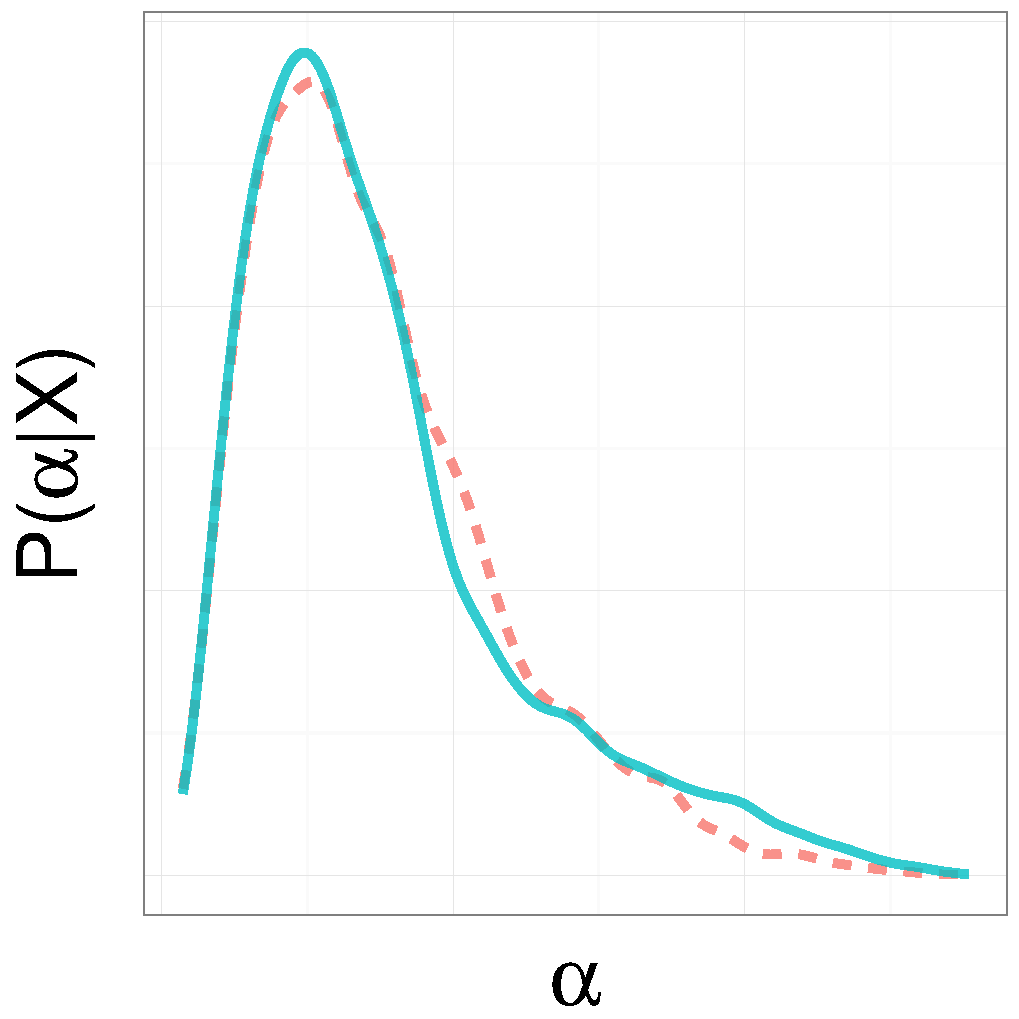
\includegraphics [width=0.49\textwidth, angle=0]{figs/EXP_ks/exp_hist_44_05_10_.pdf}
    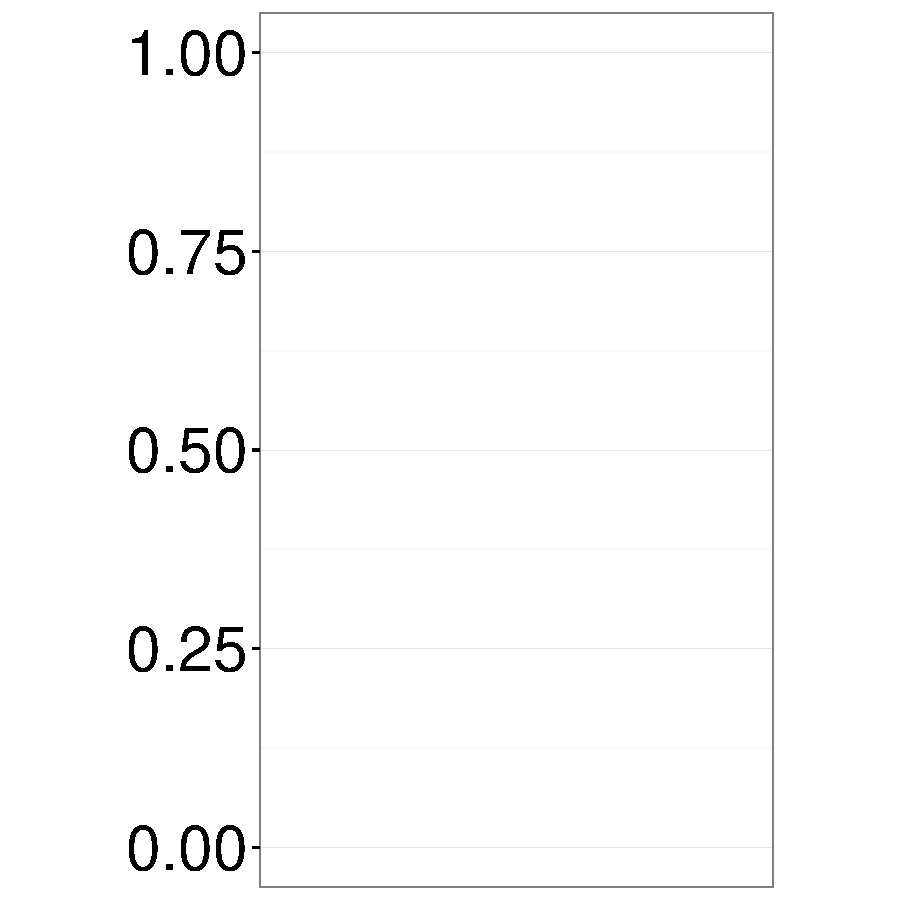
\includegraphics [width=0.49\textwidth, angle=0]{figs/acc/EXP_D10alpha_k2.pdf}
  \end{minipage}
  \begin{minipage}[!hp]{0.49\linewidth}
    \vspace{-.2in}
    \caption{(Left) posterior $P(\alpha|X)$ from Gibbs (dashed line) and symmetrized MH (solid line) for the synthetic model. (Right) acceptance probabilities of $\alpha$ for symmetrized (squares) and \naive\ (triangles) MH.} 
    \label{fig:POST_EXP}
  \end{minipage}
  \end{figure}
  \begin{figure}[H]
  \centering
  \begin{minipage}[!hp]{0.97\linewidth}
    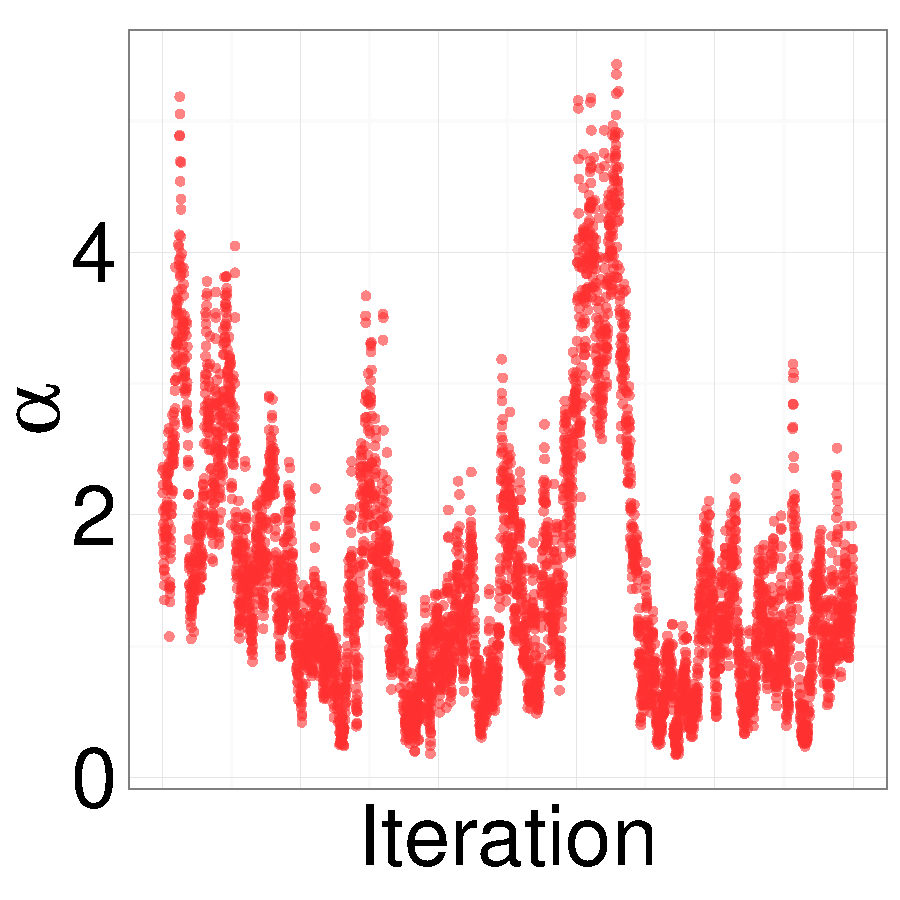
\includegraphics [width=0.24\textwidth, angle=0]{figs/EXP_ks/exp_traceGBS_44_05_10_.pdf}
    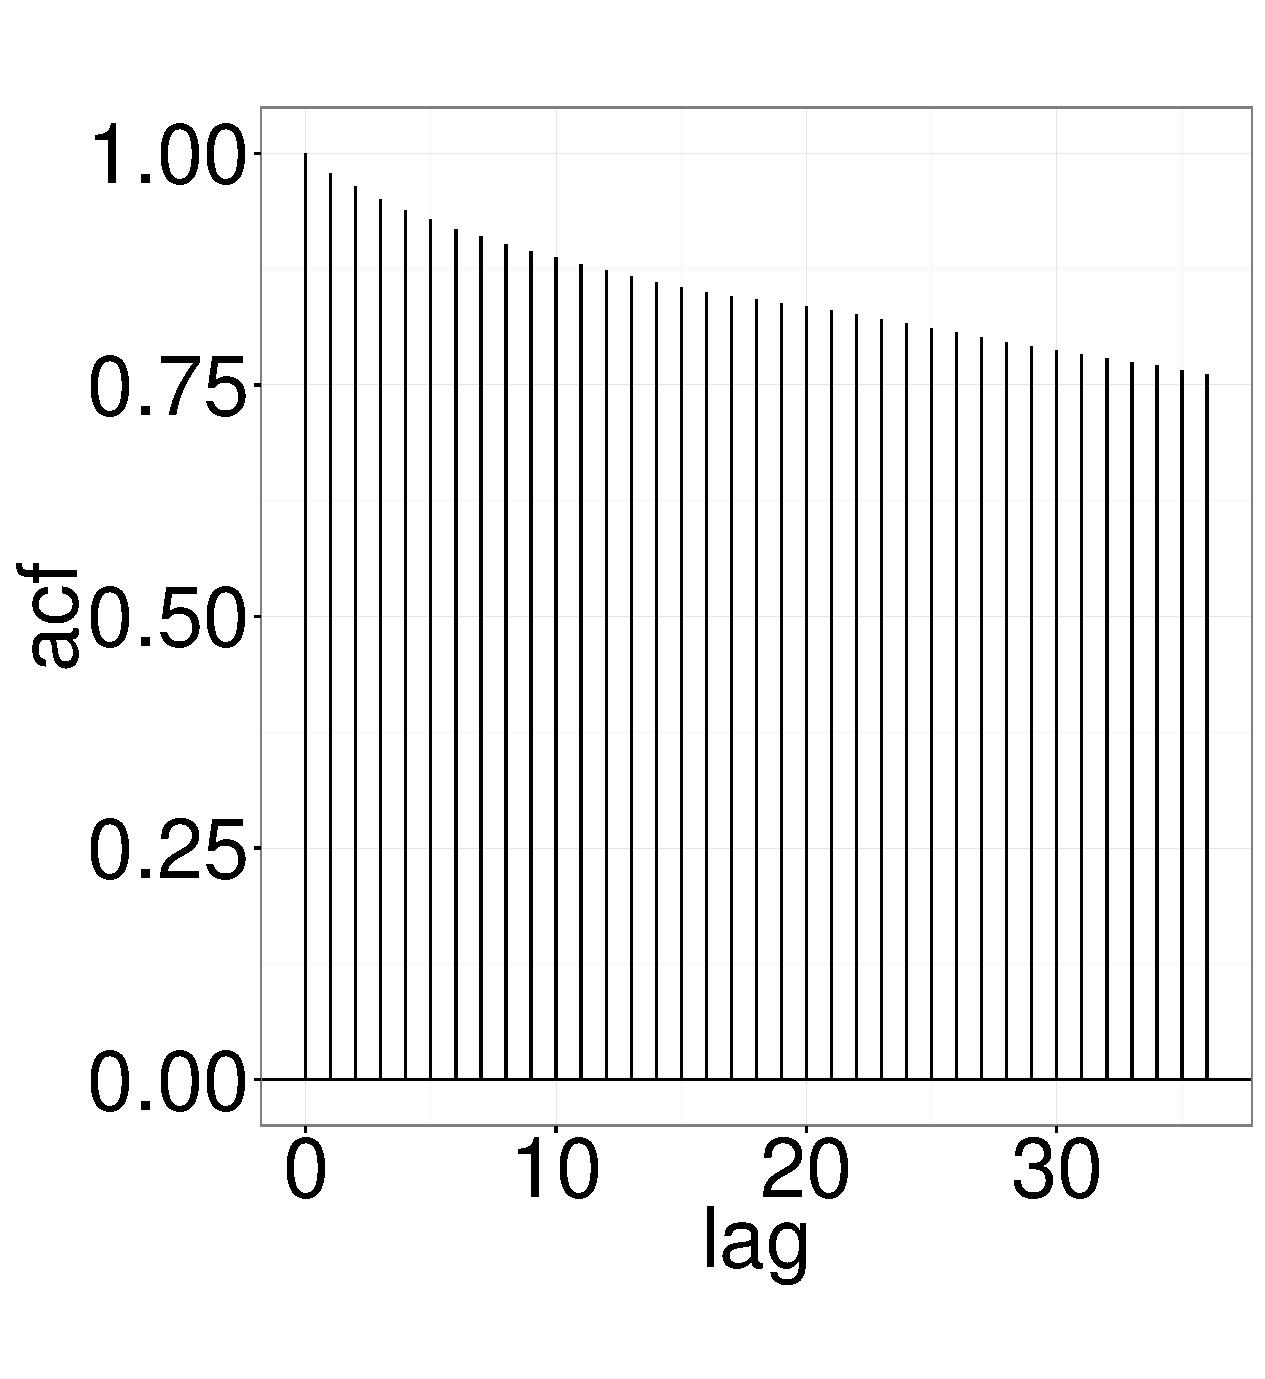
\includegraphics [width=0.24\textwidth, angle=0]{figs/EXP_ks/exp_gbsacf_44_05_10_.pdf}
    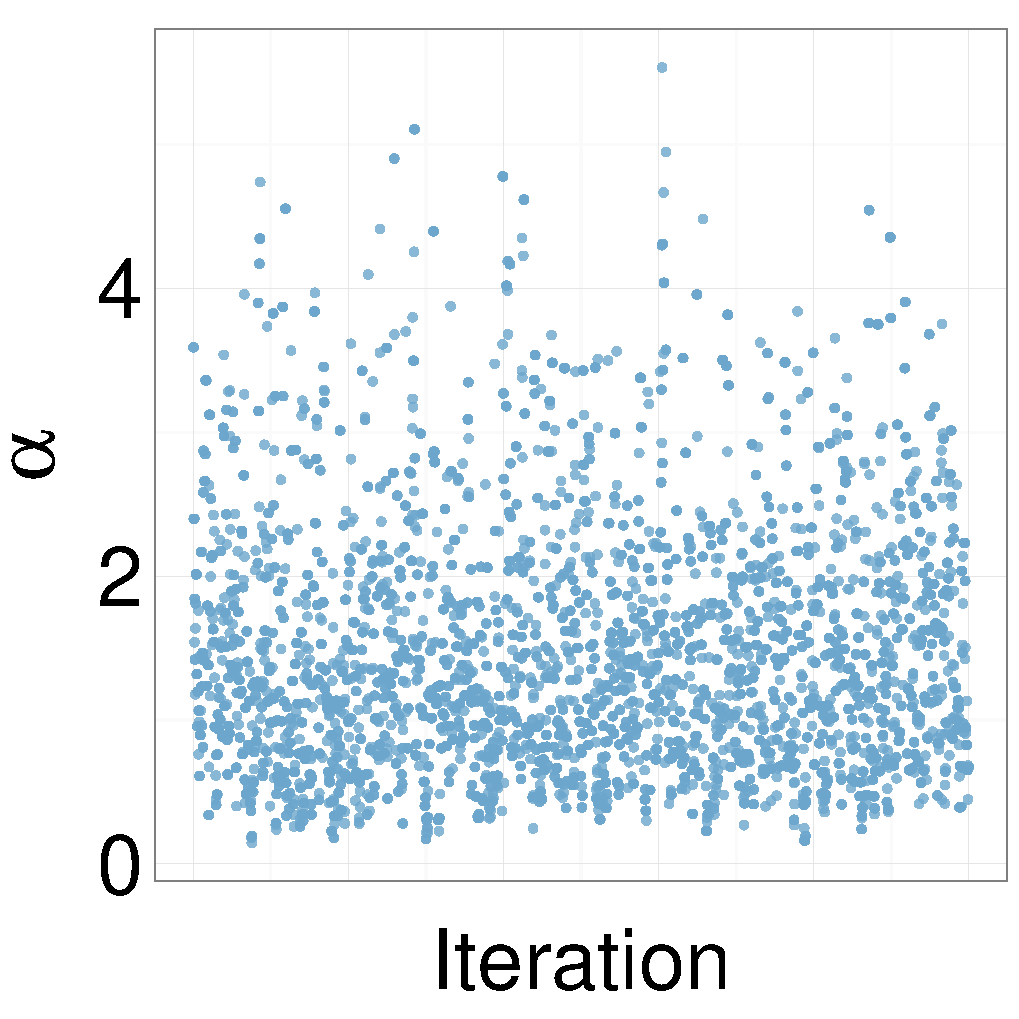
\includegraphics [width=0.24\textwidth, angle=0]{figs/EXP_ks/exp_traceMH_44_05_10_.pdf}
    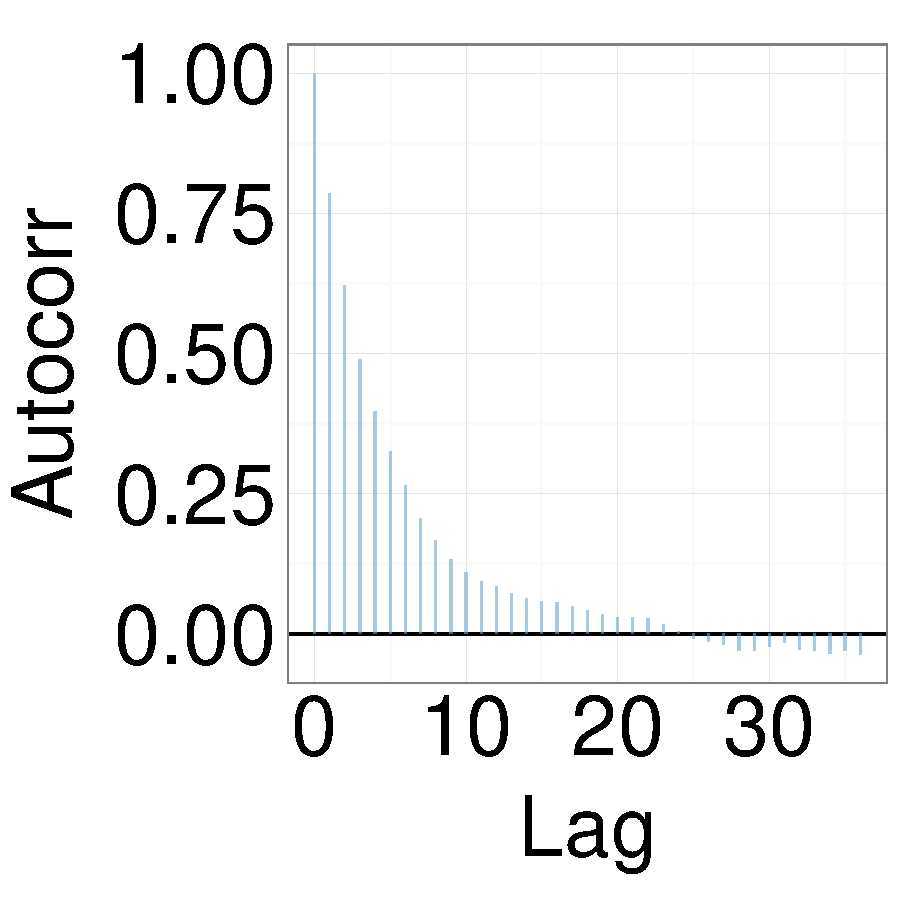
\includegraphics [width=0.24\textwidth, angle=0]{figs/EXP_ks/exp_mhacf_44_05_10_.pdf}
  \end{minipage}
  \caption{Trace and autocorrelation plots for Gibbs (left two panels) and symmetrized MH (right two panels). All plots are for the synthetic odel with $10$ states.}
     \label{fig:TRACE_EXP}
  \end{figure}
  To quantify this, figure~\ref{fig:ESS_EXP_D10} plots the ESS/sec in the top row, and the raw ESS in the bottom row for $\alpha$  and $\beta$. 
  The left two columns plot $\alpha$ and $\beta$ for MJPs with $3$ states, and the right two, with $10$ states. 
  We include results for $5$ states in the appendix, the conclusions are the same. 
  For each plot, we vary the scale-parameter $\sigma^2$ of the log-normal proposal $q(\vartheta|\theta)$, and look at its effects on ESS/s and ESS. 
  Note that the conditional over parameters given trajectory is not conjugate, so that the Gibbs sampler is really a Metropolis-within-Gibbs (MWG) sampler with an associated proposal distribution parameterized by $\sigma^2$.
  %as we change the variance of the
  %proposal kernel, for different methods and different scaling parameters.
  %($\kappa =
%1.5, 2, 3$) and dimensions($p = 3, 5, 10$).
%, where   $k = 1.5$,  $\Omega(\theta, \theta^*) = k \max(\max A(\theta), \max A(\theta^*))$. 
%For particle MCMC, the number of particles can be $5, 10 , 20$. 
%  Blue lines are the Gibbs sampler, orange lines are \naive\ MH, red lines 
%are the symmetrized MH and black lines are particle MCMC. 
%For methods involving standard uniformization (Gibbs and \naive\ MH), dots 
%correspond to $\kappa = 1$, triangles correspond to $\kappa = 2$, and squares 
%correspond to $\kappa = 1.5$. For our symmetrized MH algorithm, circles,
%triangles and squares correspond to $\Omega = (\Omega_{old} + \Omega_{new}),
%2(\Omega_{old} + \Omega_{new})$ and $1.5 \max(\Omega_{old}, \Omega_{new})$
%respectively, where $\Omega_{new}$ and $\Omega_{old}$ equal $\max_i A_i$ under 
%the proposed and current parameters.
%  For particle MCMC, the dot-dashed lines correspond to 
%  $5$ particles,  the dashed lines correspond to $10$ particles, and the solid 
%  lines correspond to $20$ particles.

  We see that our symmetrized MH algorithm, shown with blue squares, is significantly more efficient than the baselines over a wide range of $\sigma^2$ values, including the natural choice of $1$.
  Among the baselines, Gibbs (red circles) does better than \naive\ MH (yellow triangles), showing that the dependency of the Poisson grid on the MJP parameters (as indicated in figure~\ref{fig:POST_EXP}) does indeed slow down mixing. 
 This, coupled with the fact that MWG tends to have higher MH acceptance than \naive\ MH results in Gibbs having superior performance. 
  Our symmetrized MH avoids this problem at no additional computational cost.
  Particle MCMC (black diamonds) has the worst performance. 

%that for $\alpha$, the improvement of our proposed sampler is even more dramatic. 
%   For $\beta$ however, performance is comparable to Gibbs, %although it is not possible to claim one is 
%   with neither uniformly superior to the other.
  \begin{figure}[H]
%    \vspace{-.2in}
  \centering
  \begin{minipage}[!hp]{0.24\linewidth}
%  \begin{minipage}[!hp]{0.69\linewidth}

  \centering
%    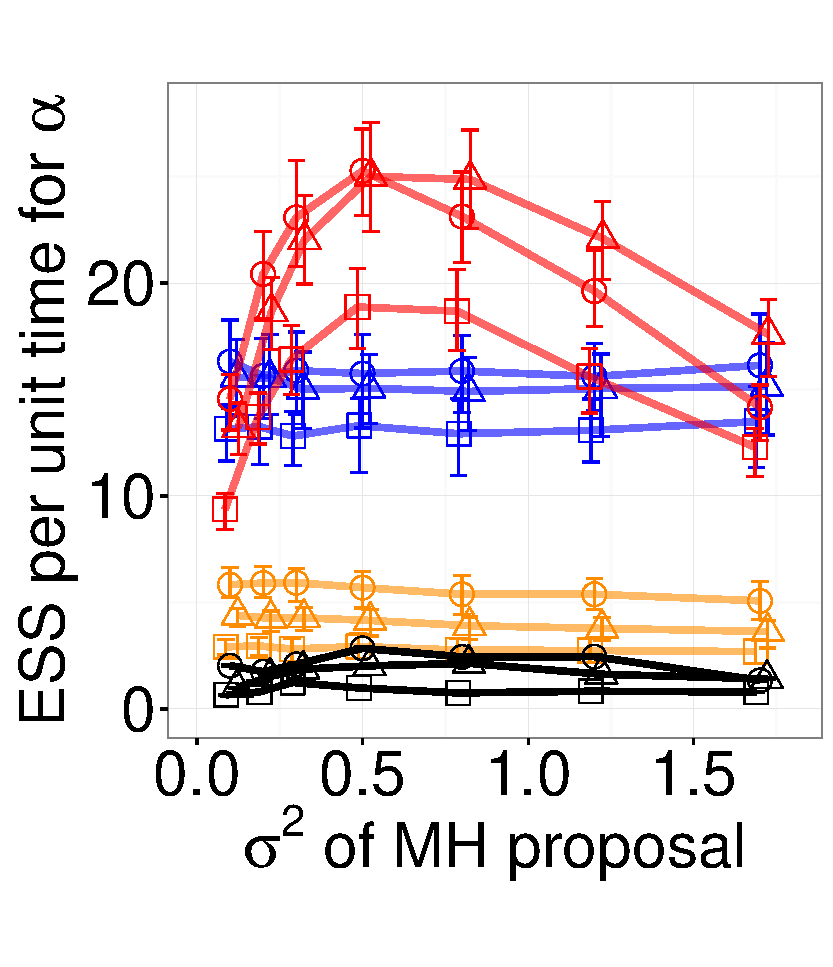
\includegraphics [width=0.49\textwidth, angle=0]{figs/exp_3_alpha.pdf}
%    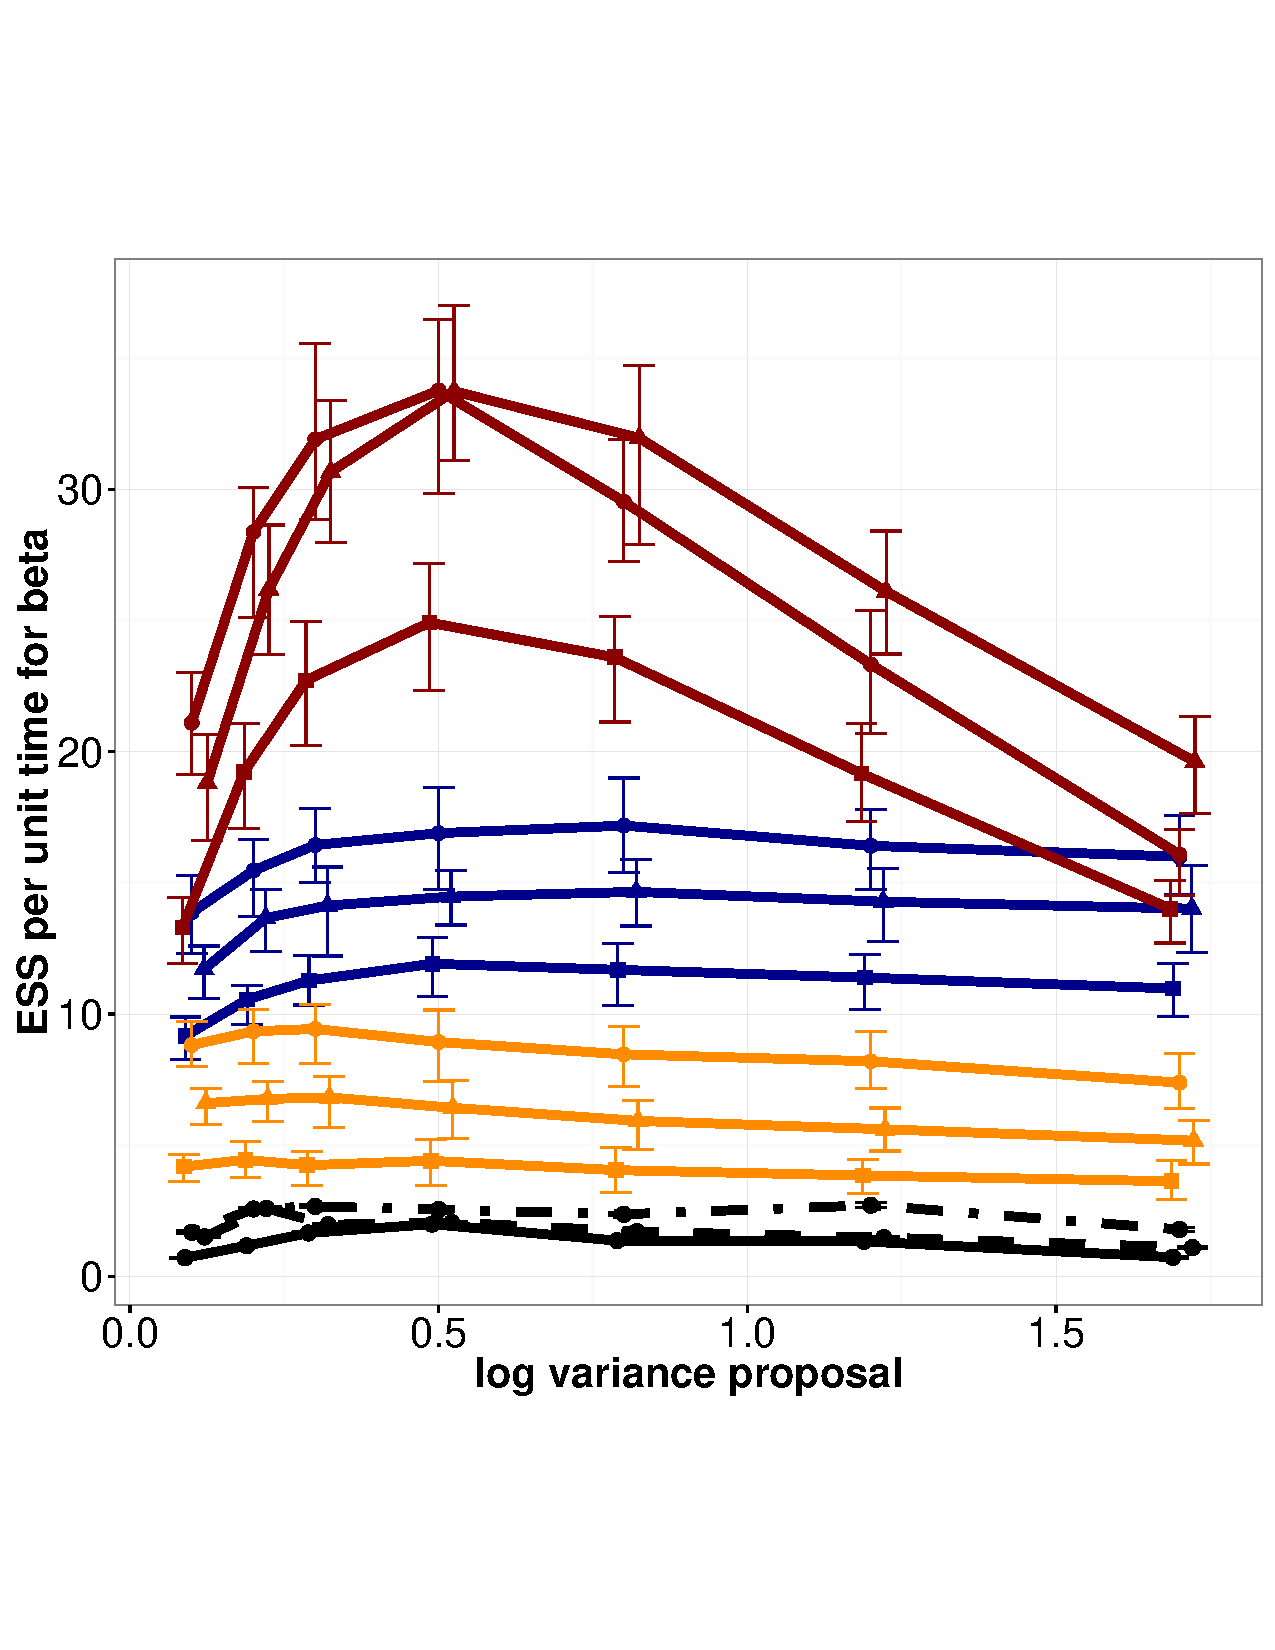
\includegraphics [width=0.49\textwidth, angle=0]{figs/exp_3_beta.pdf}
%    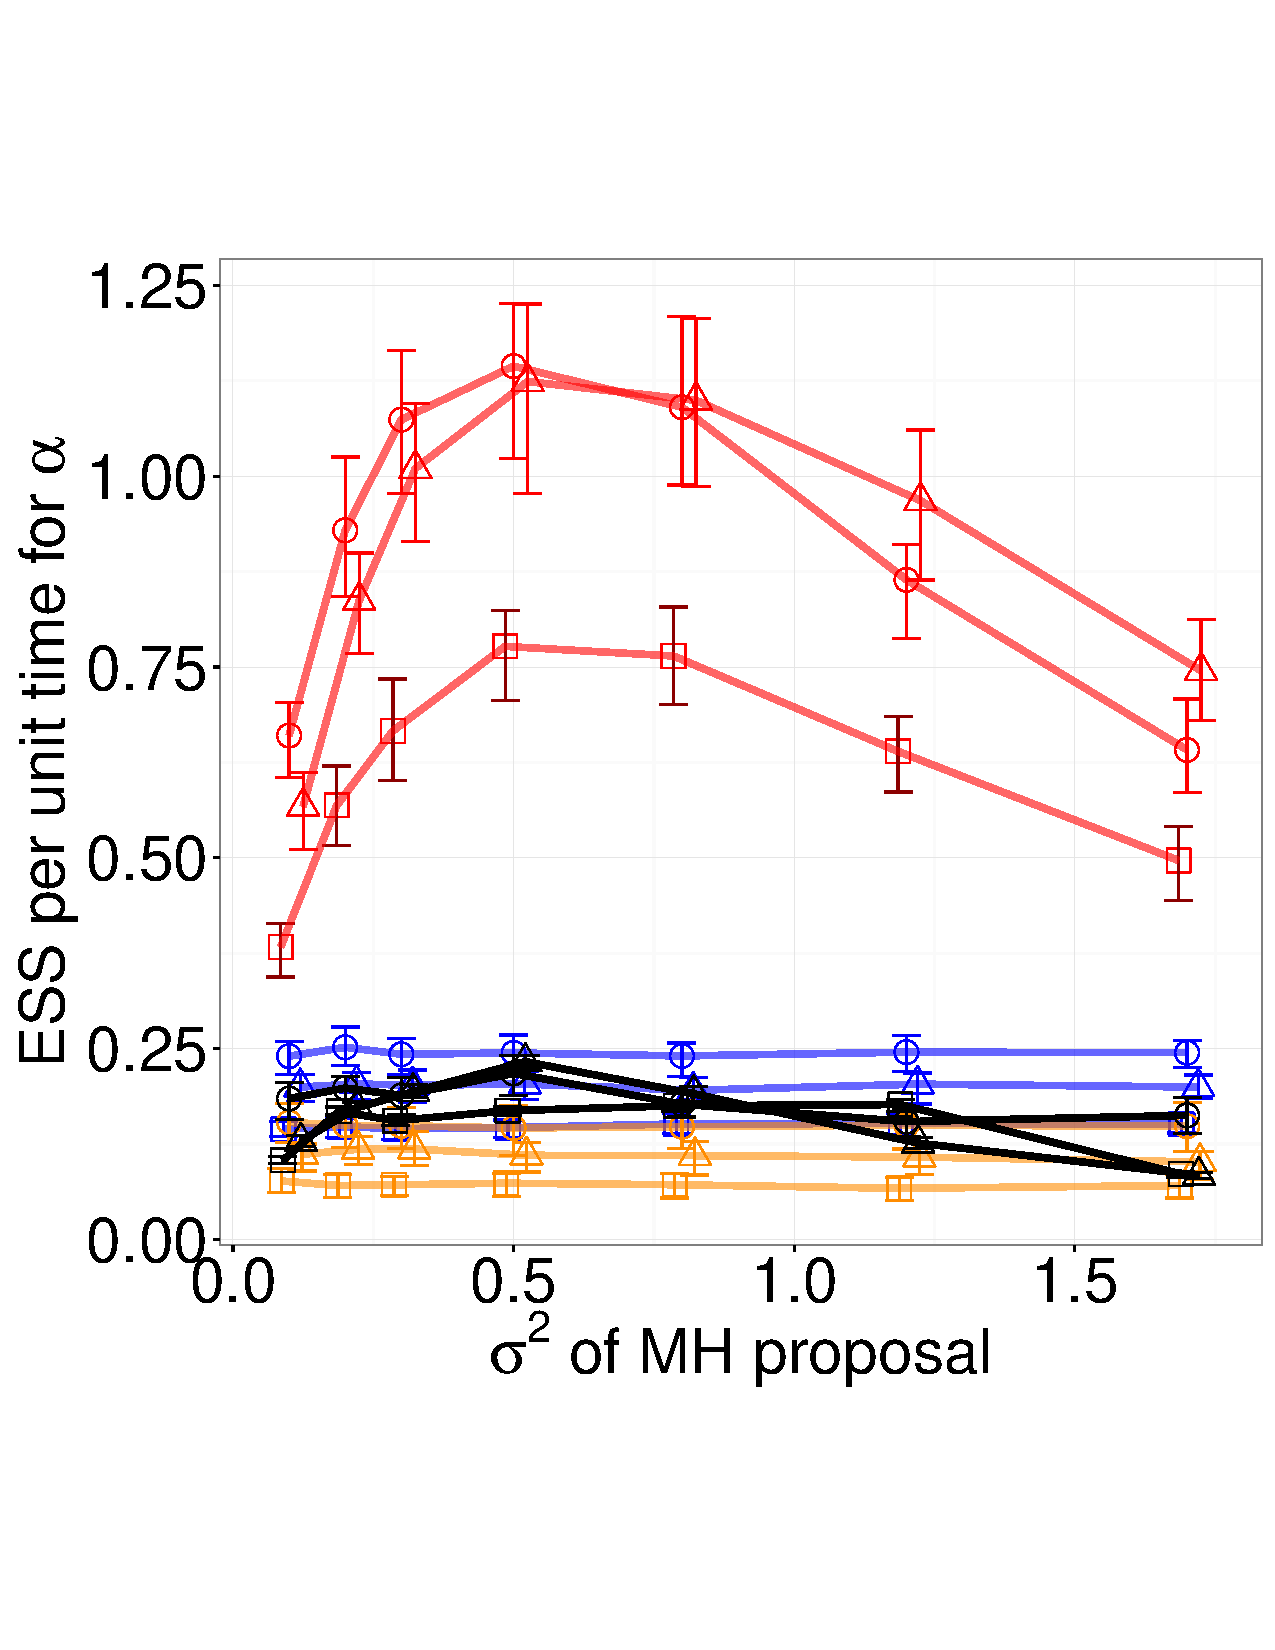
\includegraphics [width=0.49\textwidth, angle=0]{figs/exp_10_alpha.pdf}
%    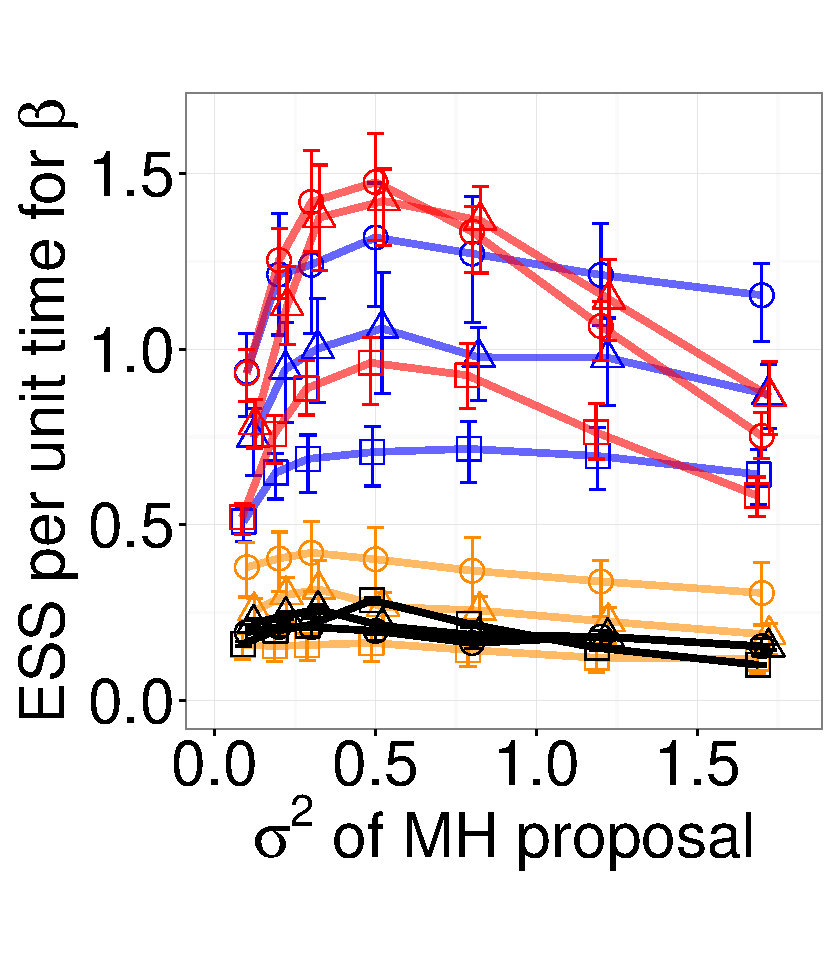
\includegraphics [width=0.49\textwidth, angle=0]{figs/exp_10_beta.pdf}
    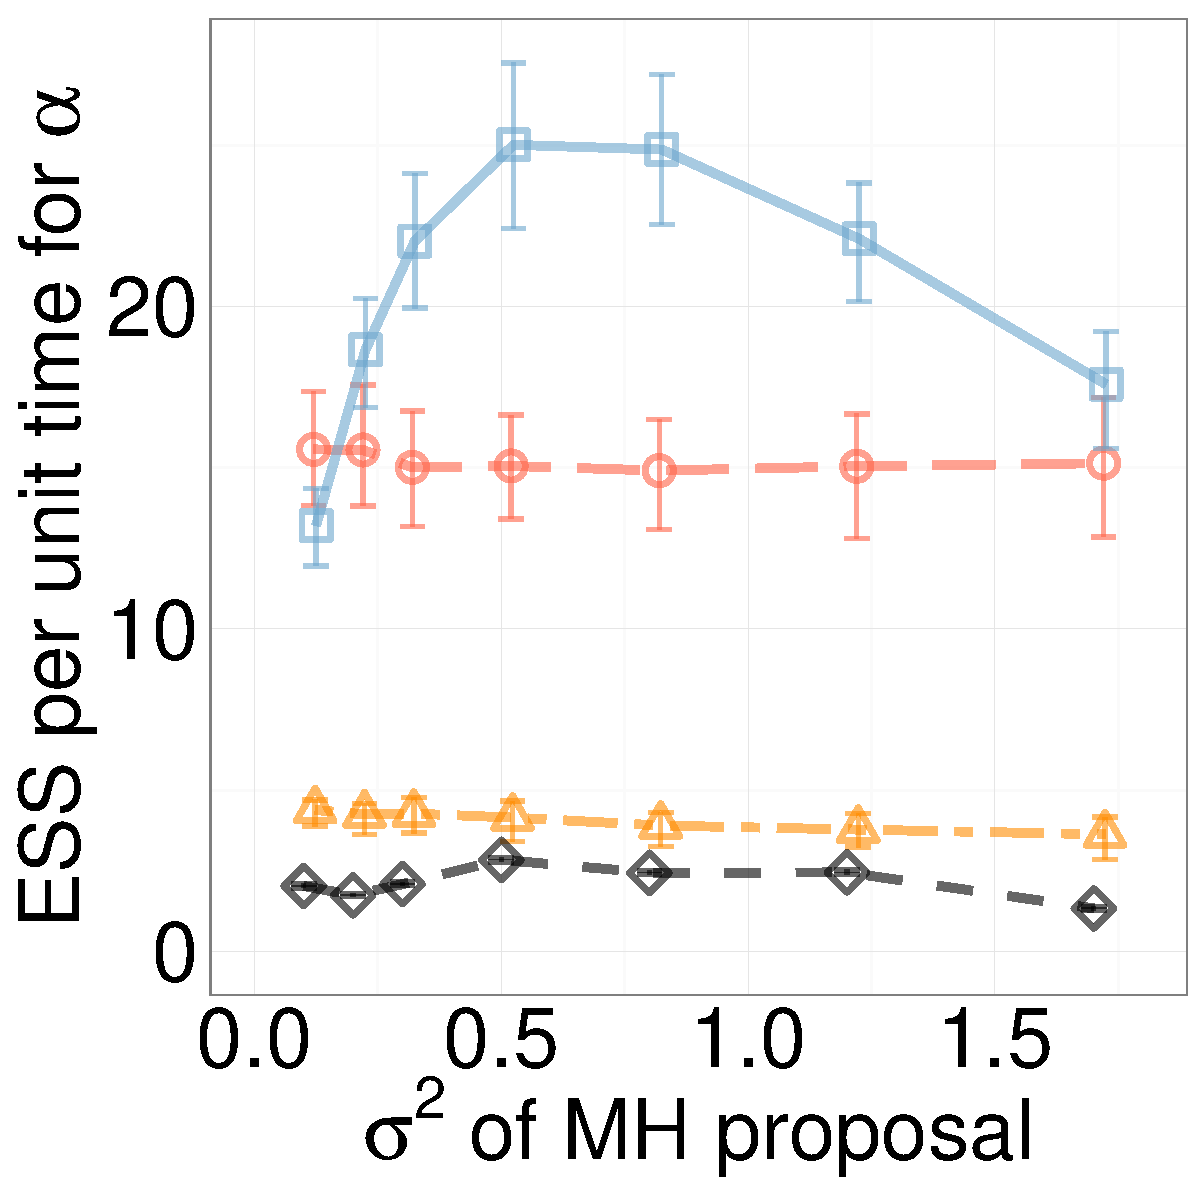
\includegraphics [width=0.99\textwidth, angle=0]{figs/new_experiment_figs/exp_alpha_dim3_k2.pdf}
\end{minipage}
  \begin{minipage}[hp]{0.24\linewidth}
  \centering
    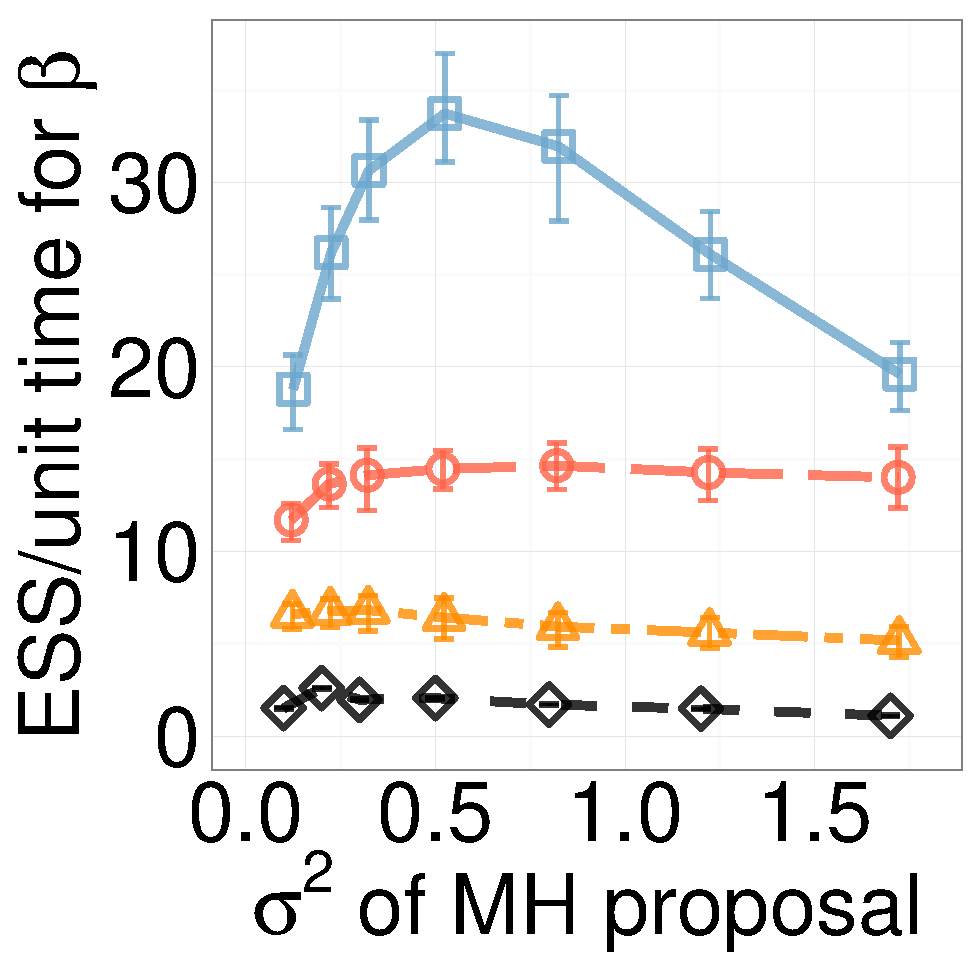
\includegraphics [width=0.99\textwidth, angle=0]{figs/new_experiment_figs/exp_beta_dim3_k2.pdf}
	\end{minipage}
  \begin{minipage}[hp]{0.24\linewidth}
  \centering
    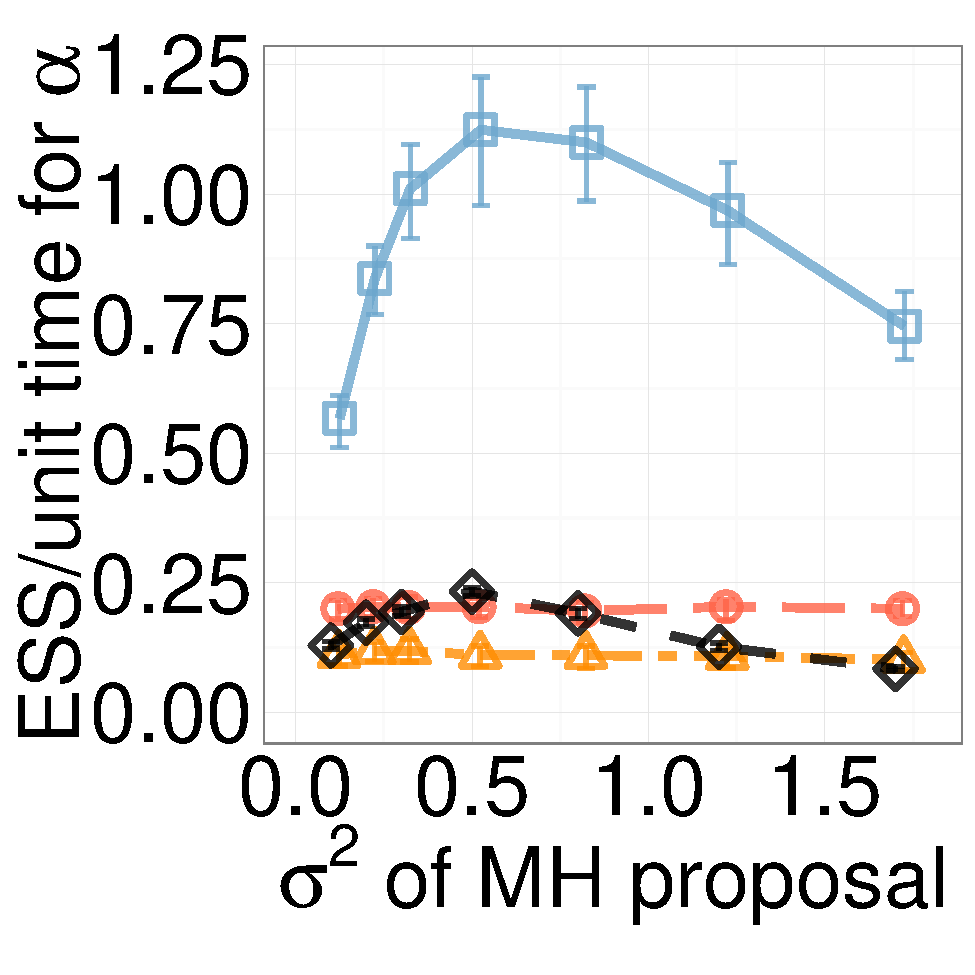
\includegraphics [width=0.99\textwidth, angle=0]{figs/new_experiment_figs/exp_alpha_dim10_k2.pdf}
	\end{minipage}
  \begin{minipage}[hp]{0.24\linewidth}
  \centering
    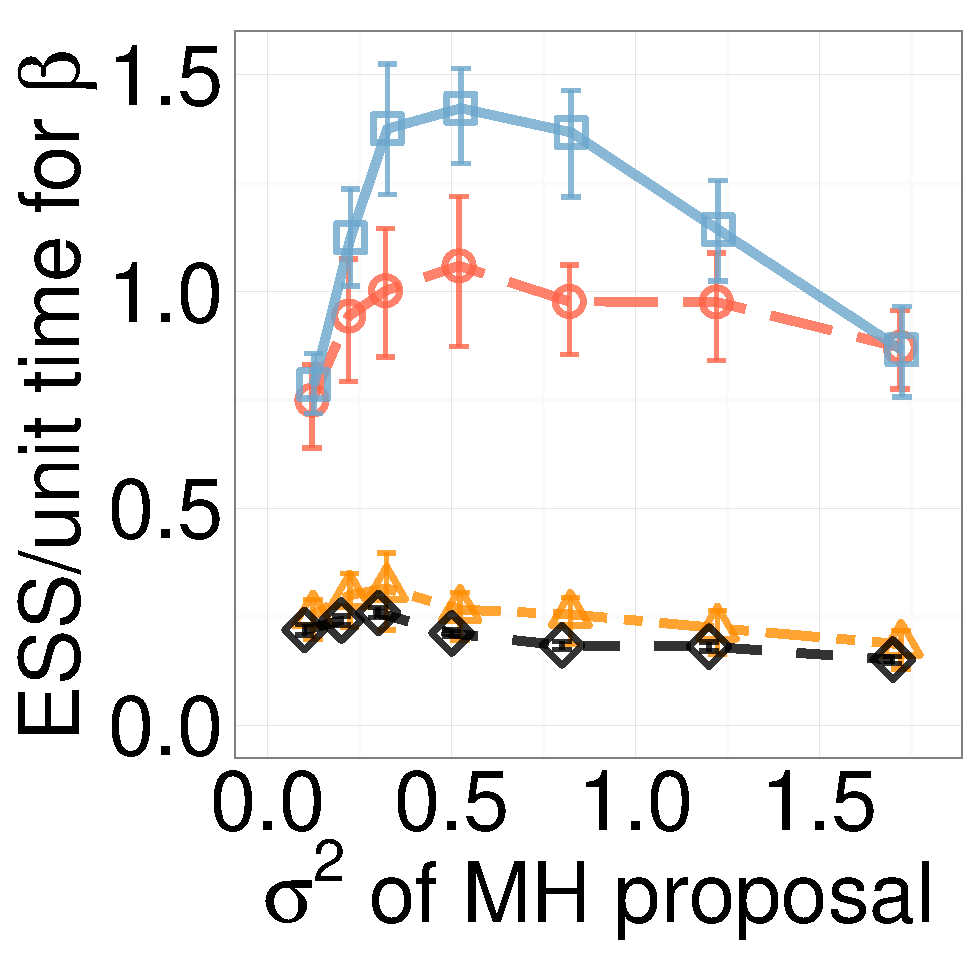
\includegraphics [width=0.99\textwidth, angle=0]{figs/new_experiment_figs/exp_beta_dim10_k2.pdf}
	\end{minipage}
%  \begin{minipage}[!hp]{0.3\linewidth}
  \centering
  \begin{minipage}[!hp]{0.24\linewidth}
  \centering
    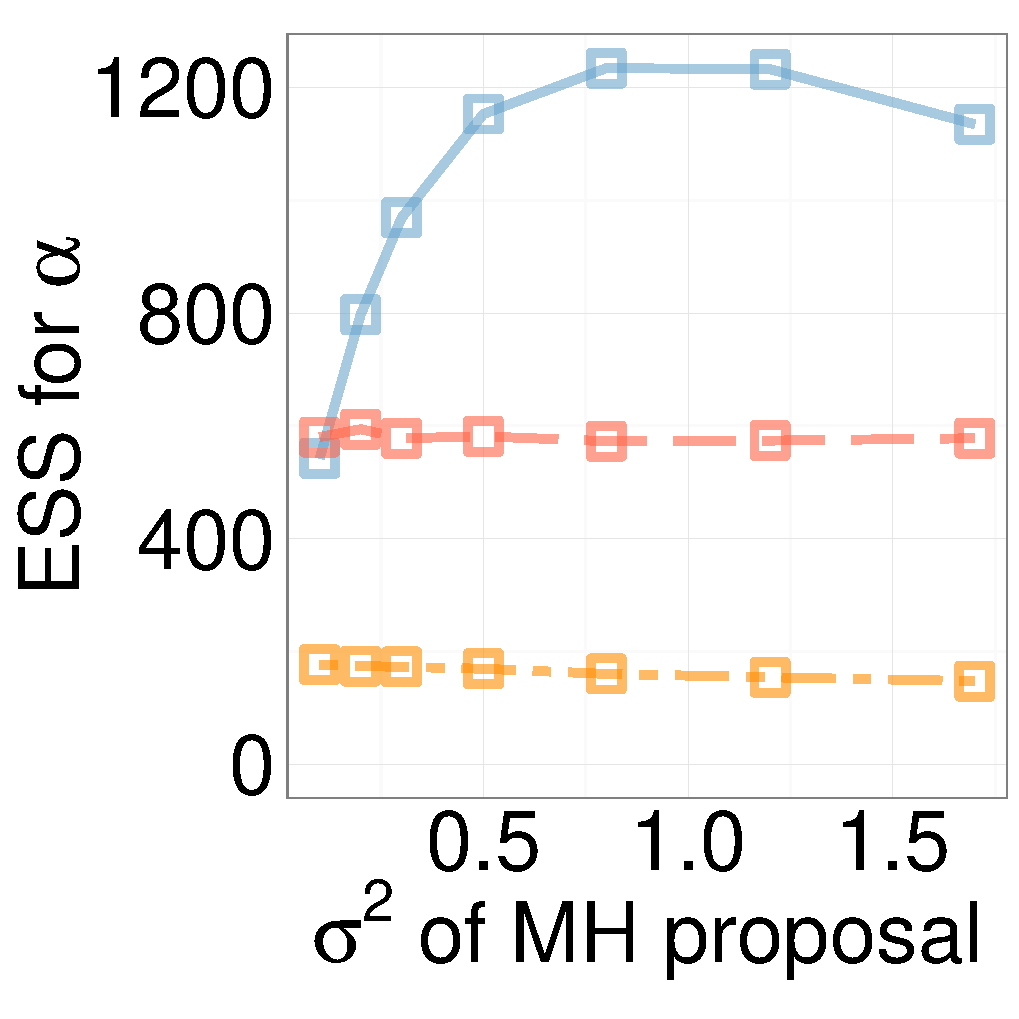
\includegraphics [width=0.99\textwidth, angle=0]{figs/ess/EXP_D3alpha_k2.pdf}
\end{minipage}
  \begin{minipage}[hp]{0.24\linewidth}
  \centering
    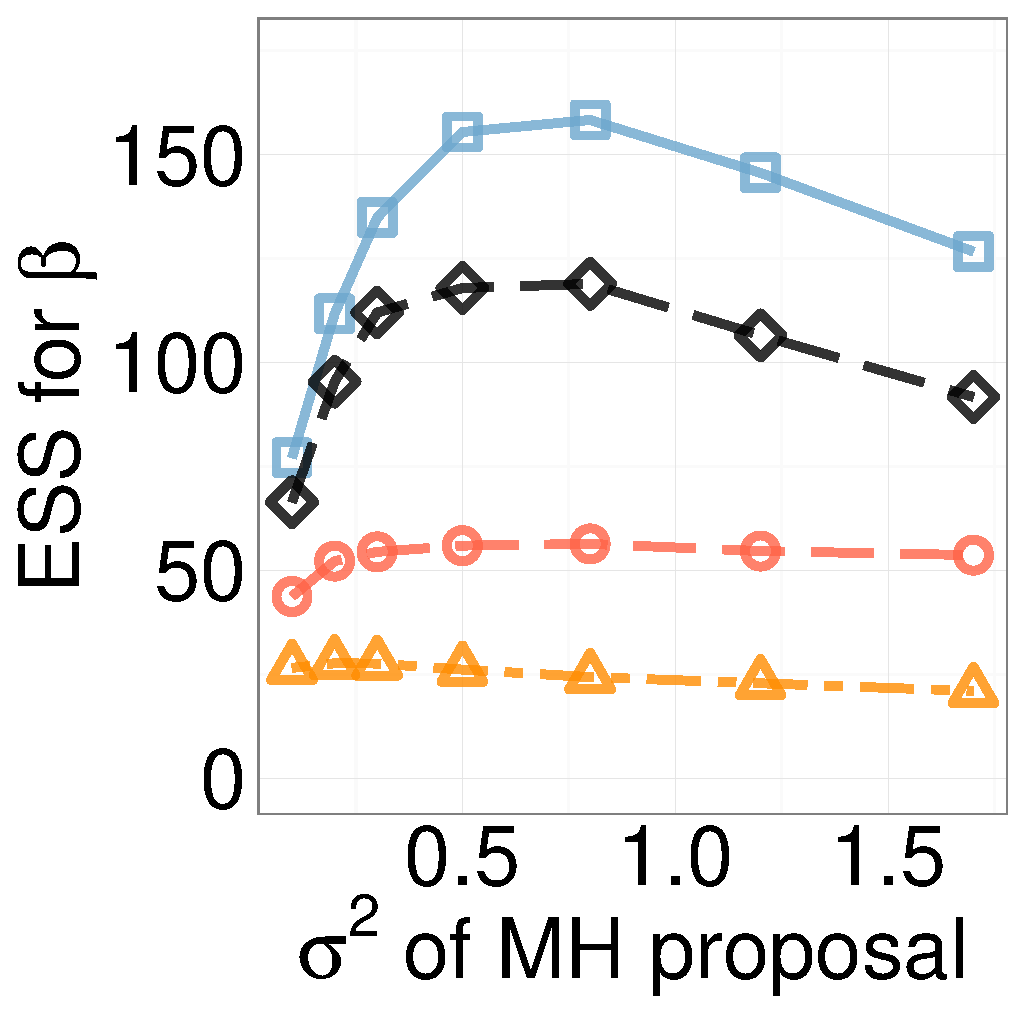
\includegraphics [width=0.99\textwidth, angle=0]{figs/ess/EXP_D3beta_k2.pdf}
	\end{minipage}
  \begin{minipage}[hp]{0.24\linewidth}
  \centering
    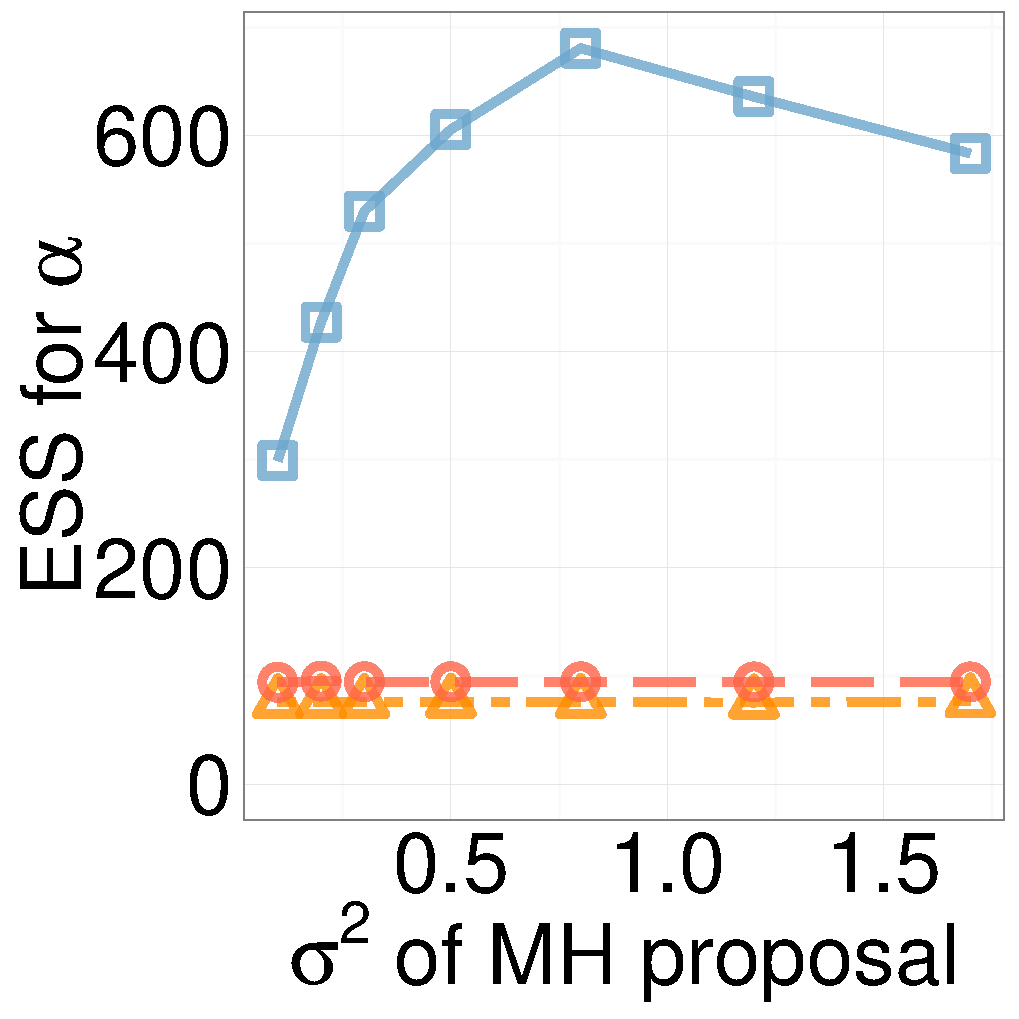
\includegraphics [width=0.99\textwidth, angle=0]{figs/ess/EXP_D10alpha_k2.pdf}
	\end{minipage}
  \begin{minipage}[hp]{0.24\linewidth}
  \centering
    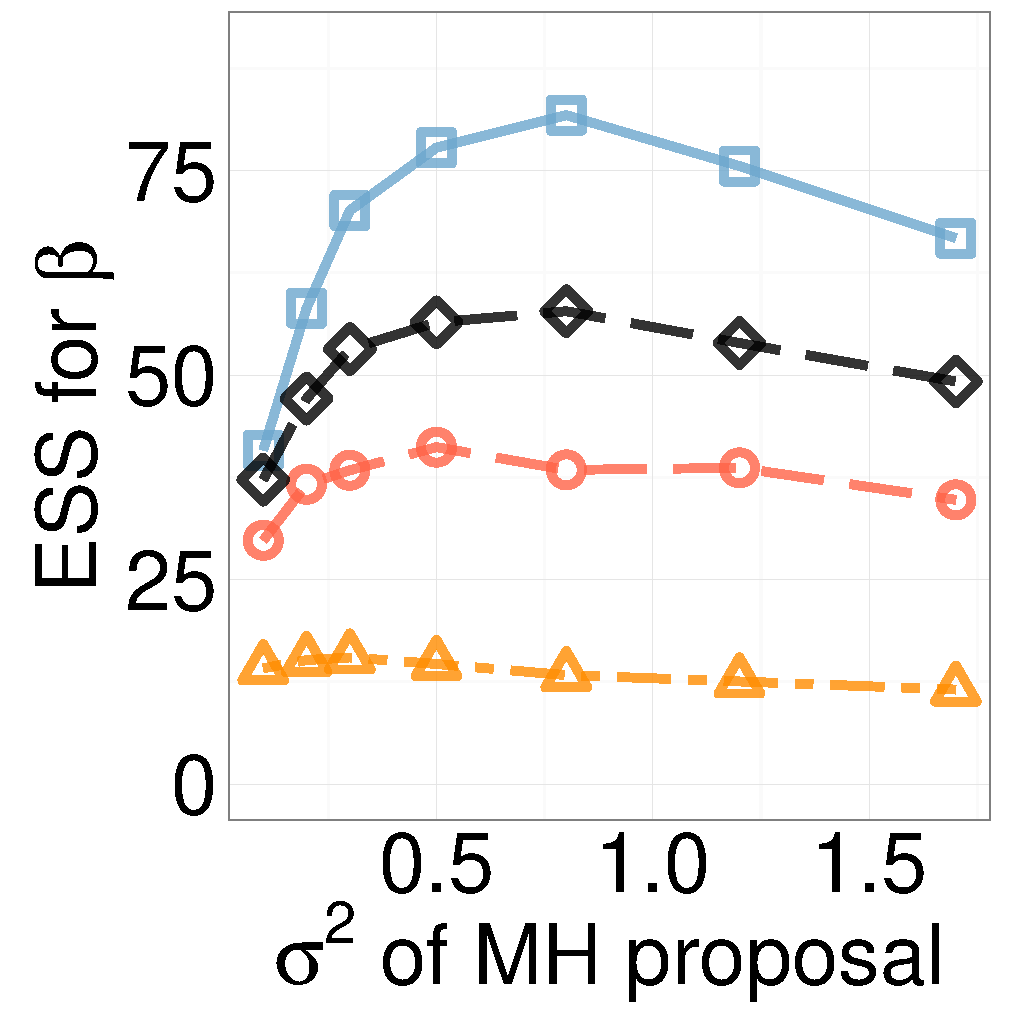
\includegraphics [width=0.99\textwidth, angle=0]{figs/ess/EXP_D10beta_k2.pdf}
	\end{minipage}
     %\label{fig:ESS_EXP_notpersec}
  \caption{ESS/sec (top row) and raw ESS per 1000 samples (bottom row) of different algorithms on the synthetic  model. The left two panels are $\alpha$ and $\beta$ for 3 states, the right two, for 10 states. Blue squares, yellow triangles, red circles and black diamonds are the symmetrized MH, \naive\ MH, Gibbs and particle MCMC algorithm.} 
%See figure~\ref{fig:} in the appendix for more results.}
     \label{fig:ESS_EXP_D10}
%  \end{minipage}
  \end{figure}

Among the three setting of our algorithm, the simple additive setting
 ({squares}) does best, though only slightly better than the {max-of-max} setting (circles). 
%A reason for this improvement is that the additive setting is more stable than the max-of-max setting, when the proposal variance can be large. 
The {additive setting with a multiplicative factor of $1.5$} ({triangles}) does worse than both the {additive choice with $\kappa=1$ and the max-of-max choice} but still better than the other algorithms. 
The results in figure~\ref{fig:ESS_EXP_D10} for 10 states shows the ESS is slightly lower, and thus mixing is slightly poorer for all samplers. This, coupled with greater computational cost per iteration results in a drop in ESS/s across all algorithms, compared to the case with 3 states. We still observe the same pattern of relative performance, with our sampler with $\Omega(\theta,\vartheta) = \max_s A_s(\theta) + \max_s A(\vartheta)$ performing the best. 

  \begin{figure}[H]
  \centering
  \begin{minipage}[!hp]{0.24\linewidth}
  \centering
    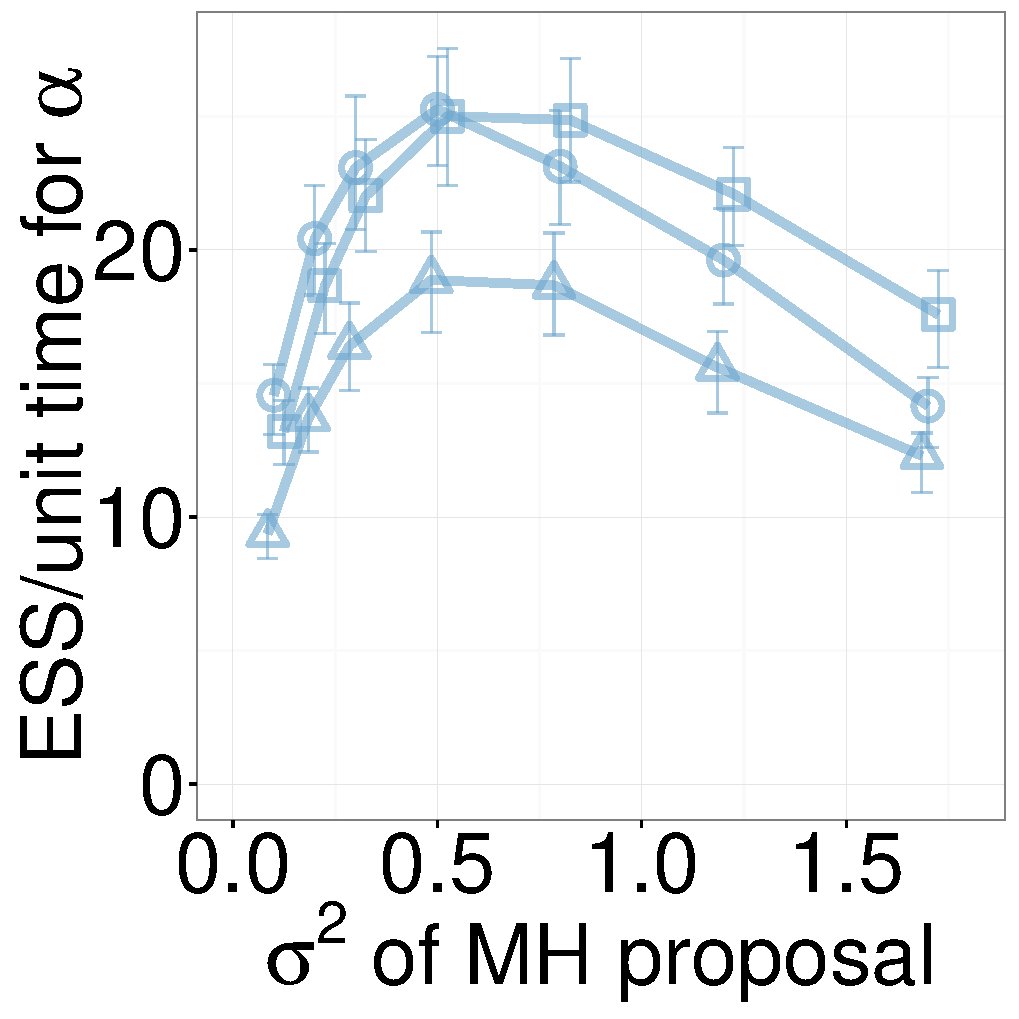
\includegraphics [width=0.99\textwidth, angle=0]{figs/new_whole_exp_figs/mh_exp_alpha_dim3.pdf}
\end{minipage}
  \begin{minipage}[hp]{0.24\linewidth}
  \centering
    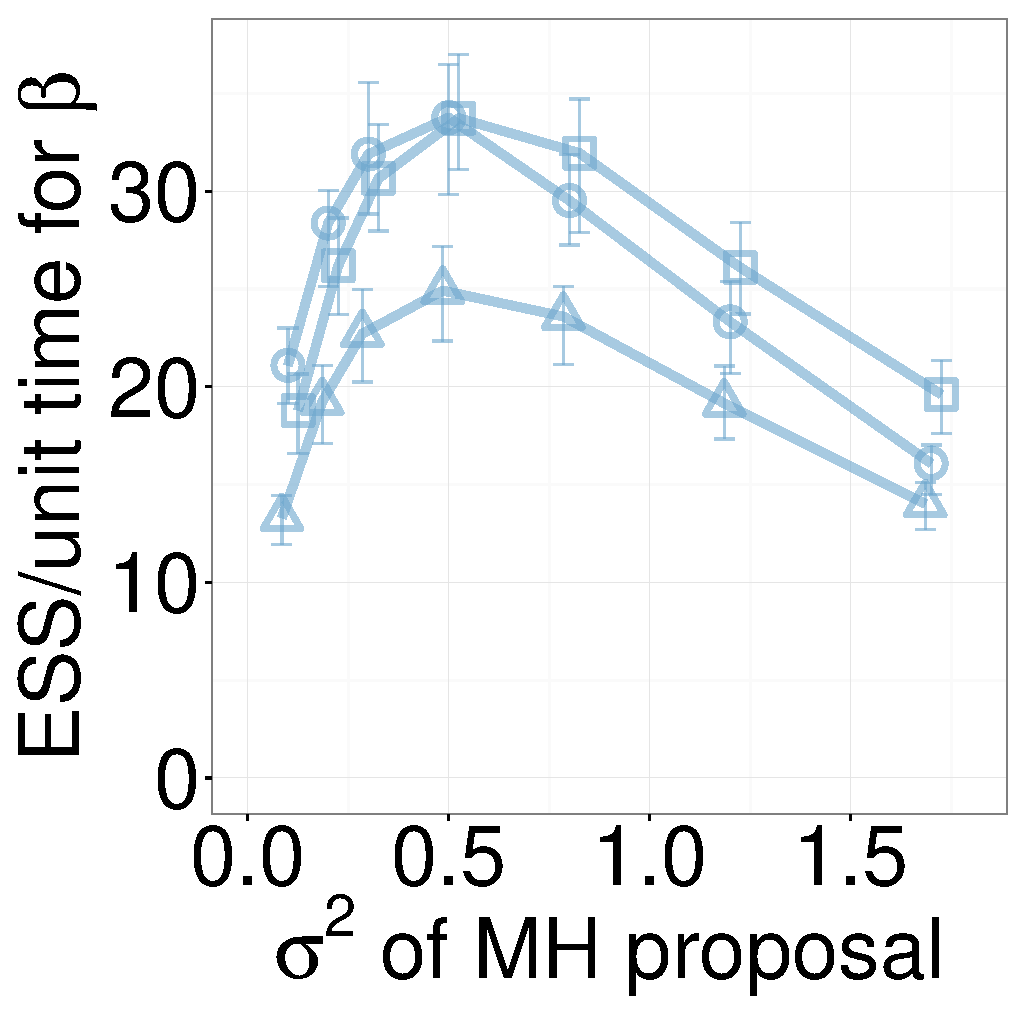
\includegraphics [width=0.99\textwidth, angle=0]{figs/new_whole_exp_figs/mh_exp_beta_dim3.pdf}
	\end{minipage}
  \begin{minipage}[hp]{0.24\linewidth}
  \centering
    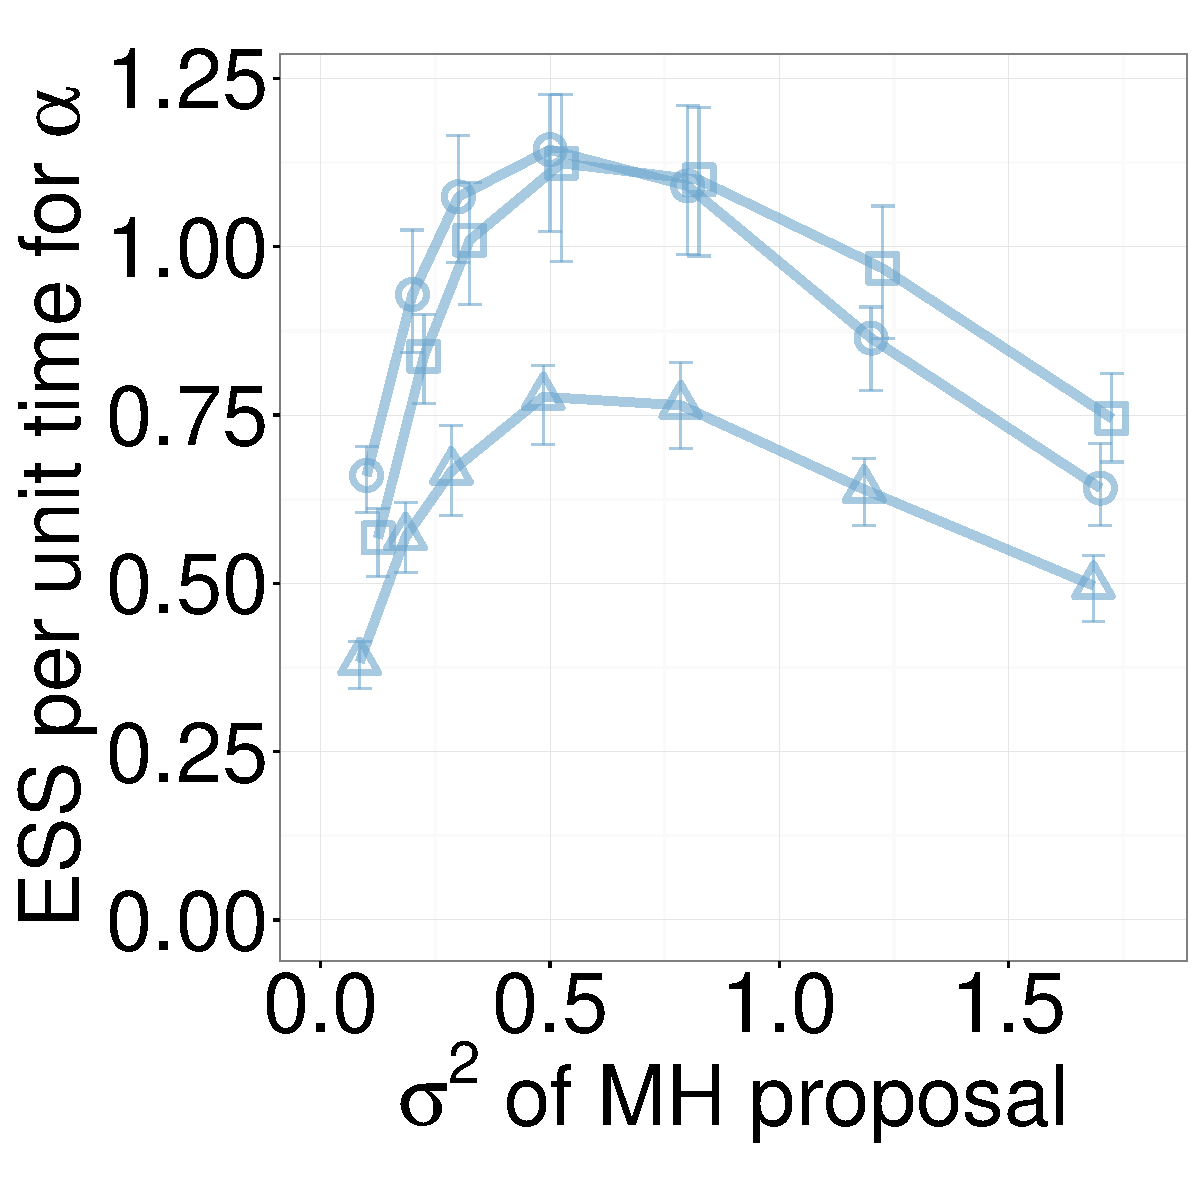
\includegraphics [width=0.99\textwidth, angle=0]{figs/new_whole_exp_figs/mh_exp_alpha_dim10.pdf}
	\end{minipage}
  \begin{minipage}[hp]{0.24\linewidth}
  \centering
    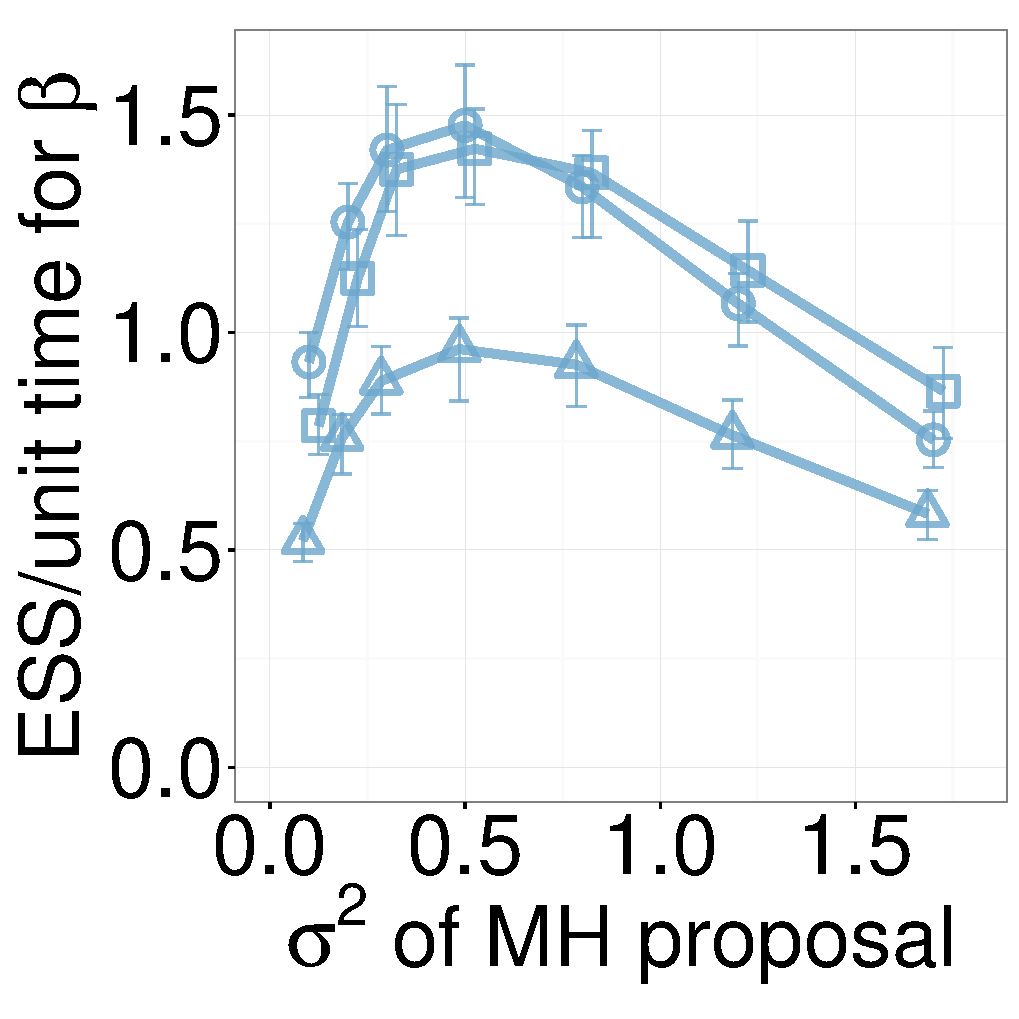
\includegraphics [width=0.99\textwidth, angle=0]{figs/new_whole_exp_figs/mh_exp_beta_dim10.pdf}
	\end{minipage}
    \caption{ESS/sec of symmetrized MH for different choices of $\Omega(\theta,\vartheta)$ for the synthetic model. The left two panels are $\alpha$ and $\beta$ for 3 states, and the right two for 10 states. Squares, circles and trianges correspond to $\Omega(\theta,\vartheta)$ set to $(\max_s A_s(\theta) + \max_s A_s(\vartheta))$, $\max(\max_s A_s(\theta), \max_s A_s(\vartheta))$ and  $1.5(\max_s A_s(\theta) + \max_s A_s(\vartheta))$.}
     \label{fig:mhESS_EXP}
  \end{figure}

%  \begin{figure}[H]
%    \vspace{-.2in}
%  \centering
 % \begin{minipage}[!hp]{0.99\linewidth}
%  \centering
 % \begin{minipage}[!hp]{0.99\linewidth}
   % 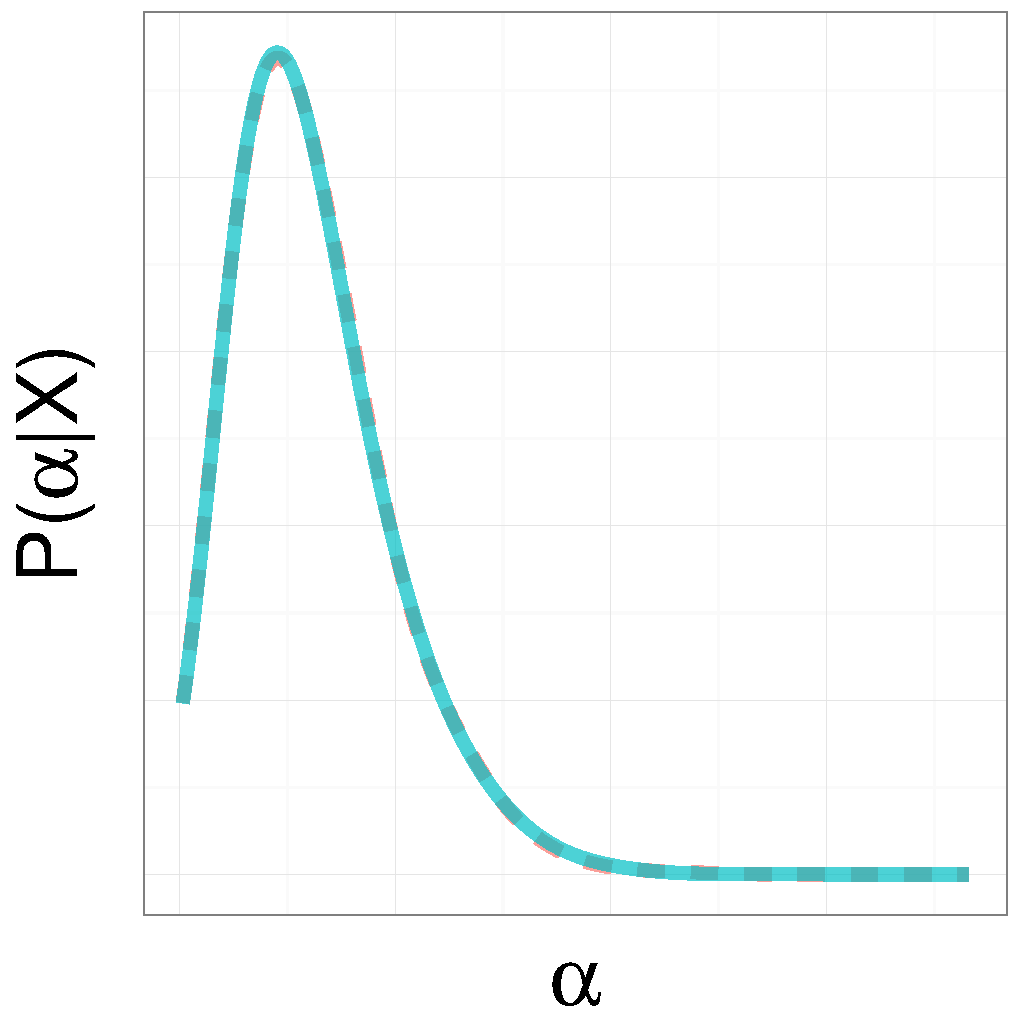
\includegraphics [width=0.45\textwidth, angle=0]{figs/EXP_ks/exp_hist_7_05_3_.pdf}
    %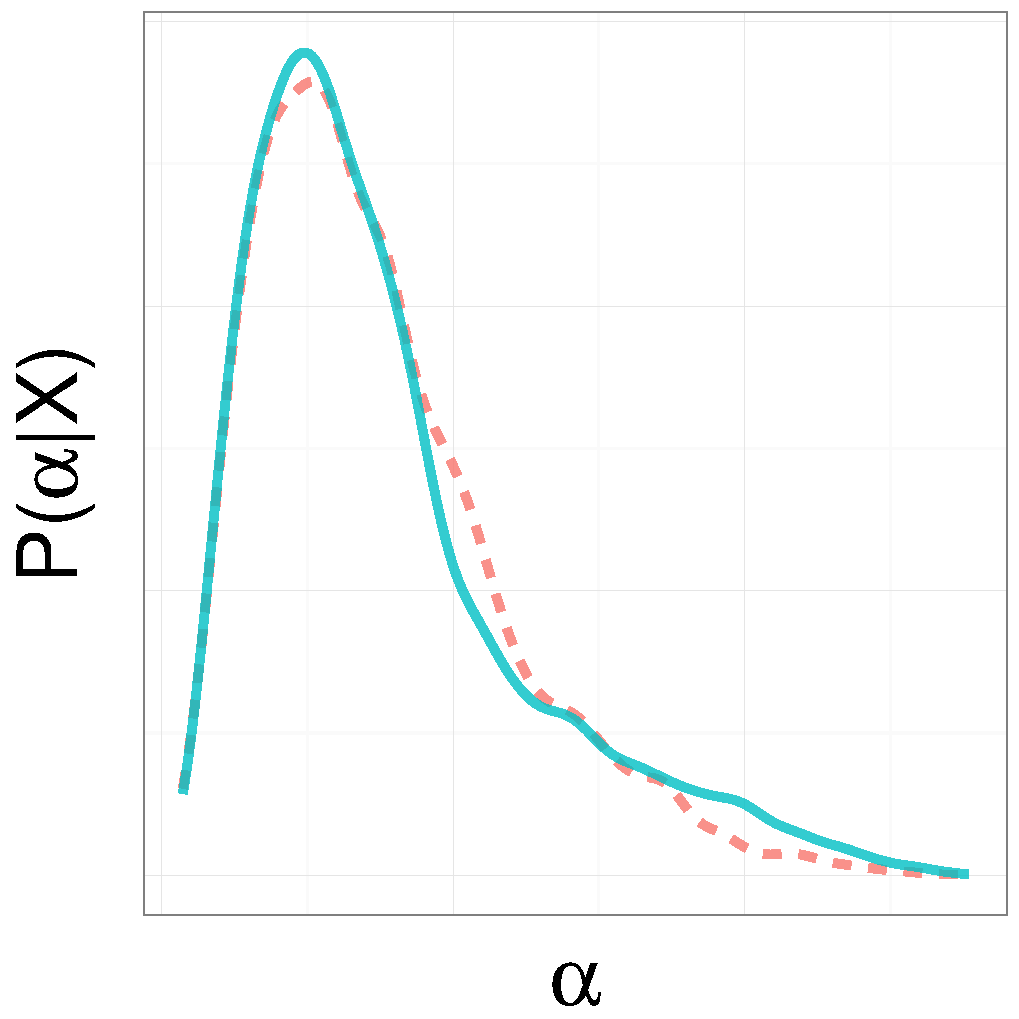
\includegraphics [width=0.45\textwidth, angle=0]{figs/EXP_ks/exp_hist_44_05_10_.pdf}
  %\end{minipage}

%  \end{minipage}
%  \begin{minipage}[!hp]{0.99\linewidth}
    %\caption{Histograms for the posterior samples of the synthetic model, the left being dimension 3 and the right being dimension 10. The red and blue curves are the Gibbs and symmetrized MH}
%     \label{fig:HIST_EXP}
%  \end{minipage}
%  \end{figure}

  \begin{figure}[H]    
  \centering
  \begin{minipage}[hp]{0.24\linewidth}
  \centering
    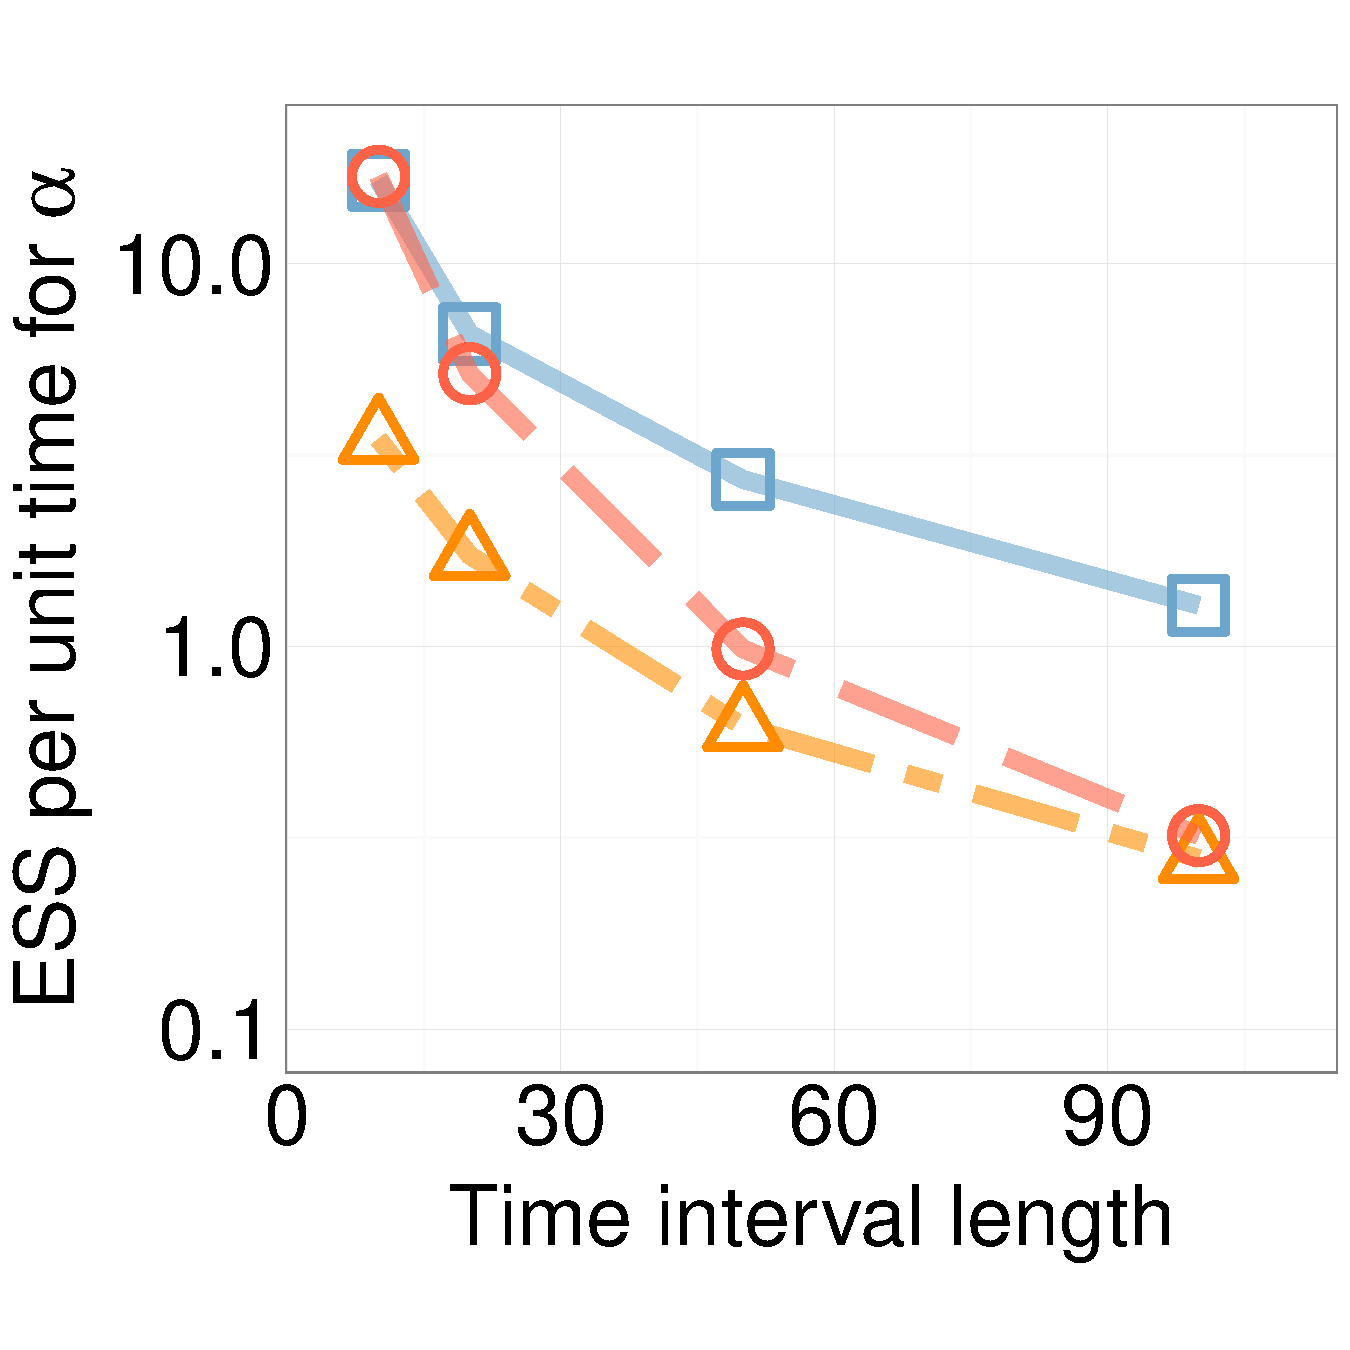
\includegraphics [width=0.99\textwidth, angle=0]{figs/new_experiment_figs/ESS_vs_t_alpha_fixobservation.pdf}
    \end{minipage}
  \begin{minipage}[hp]{0.24\linewidth}
  \centering
    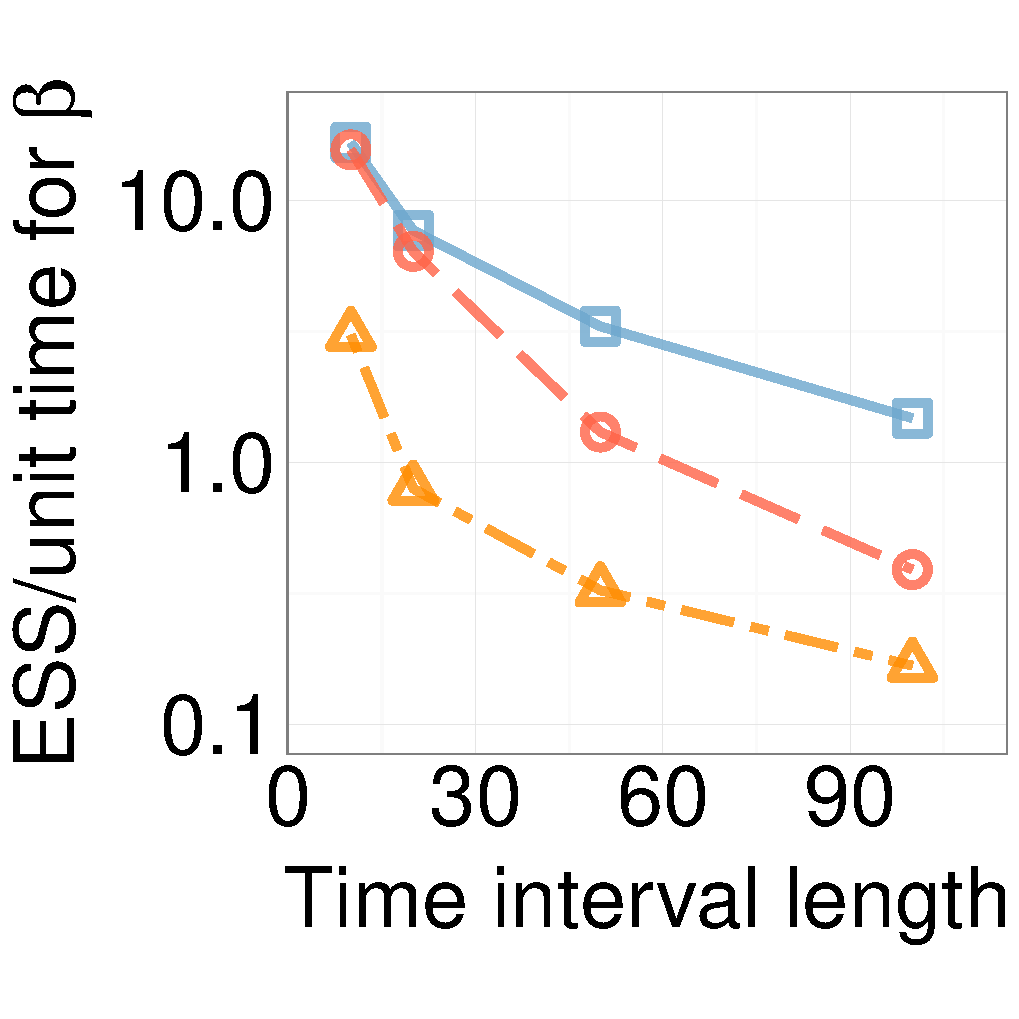
\includegraphics [width=0.99\textwidth, angle=0]{figs/new_experiment_figs/ESS_vs_t_beta_fixobservation.pdf}
%    \vspace{-0.3in}
  \end{minipage}
    %\label{fig:TSS_fix}
  \begin{minipage}[hp]{0.24\linewidth}
  \centering
    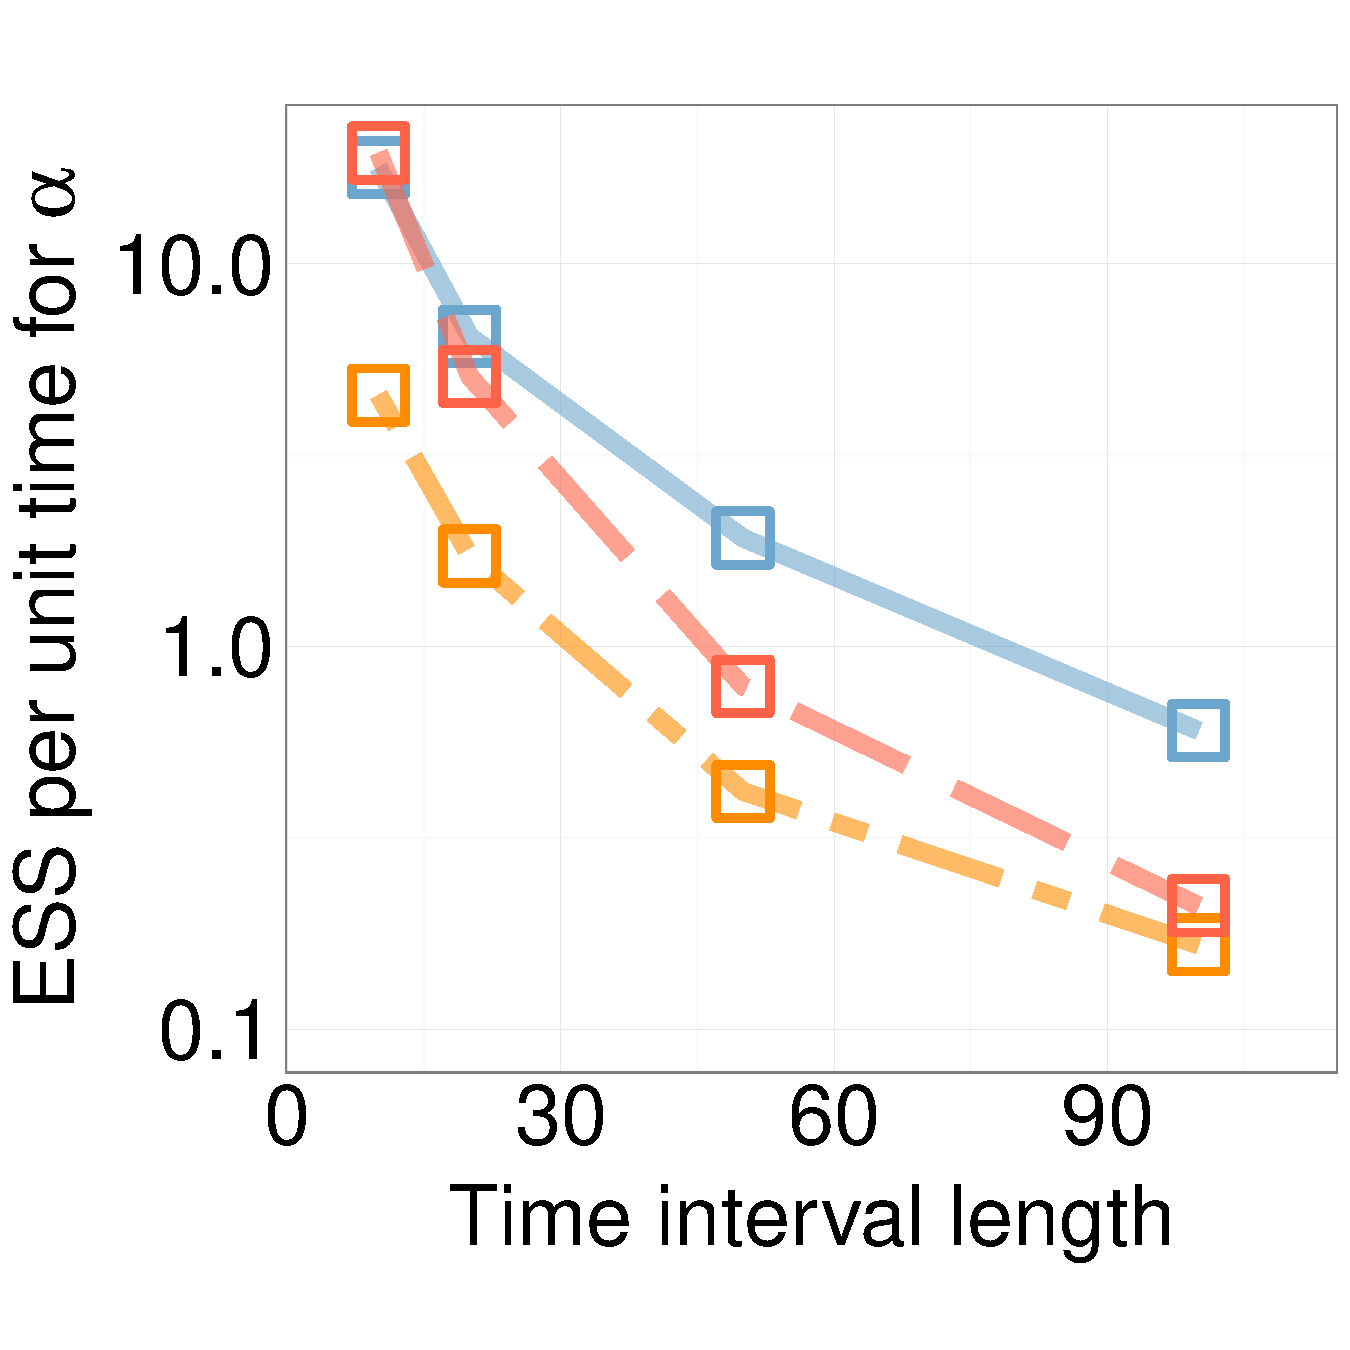
\includegraphics [width=0.99\textwidth, angle=0]{figs/new_experiment_figs/ESS_vs_t_alpha.pdf}
      \end{minipage}
  \begin{minipage}[hp]{0.24\linewidth}
  \centering
    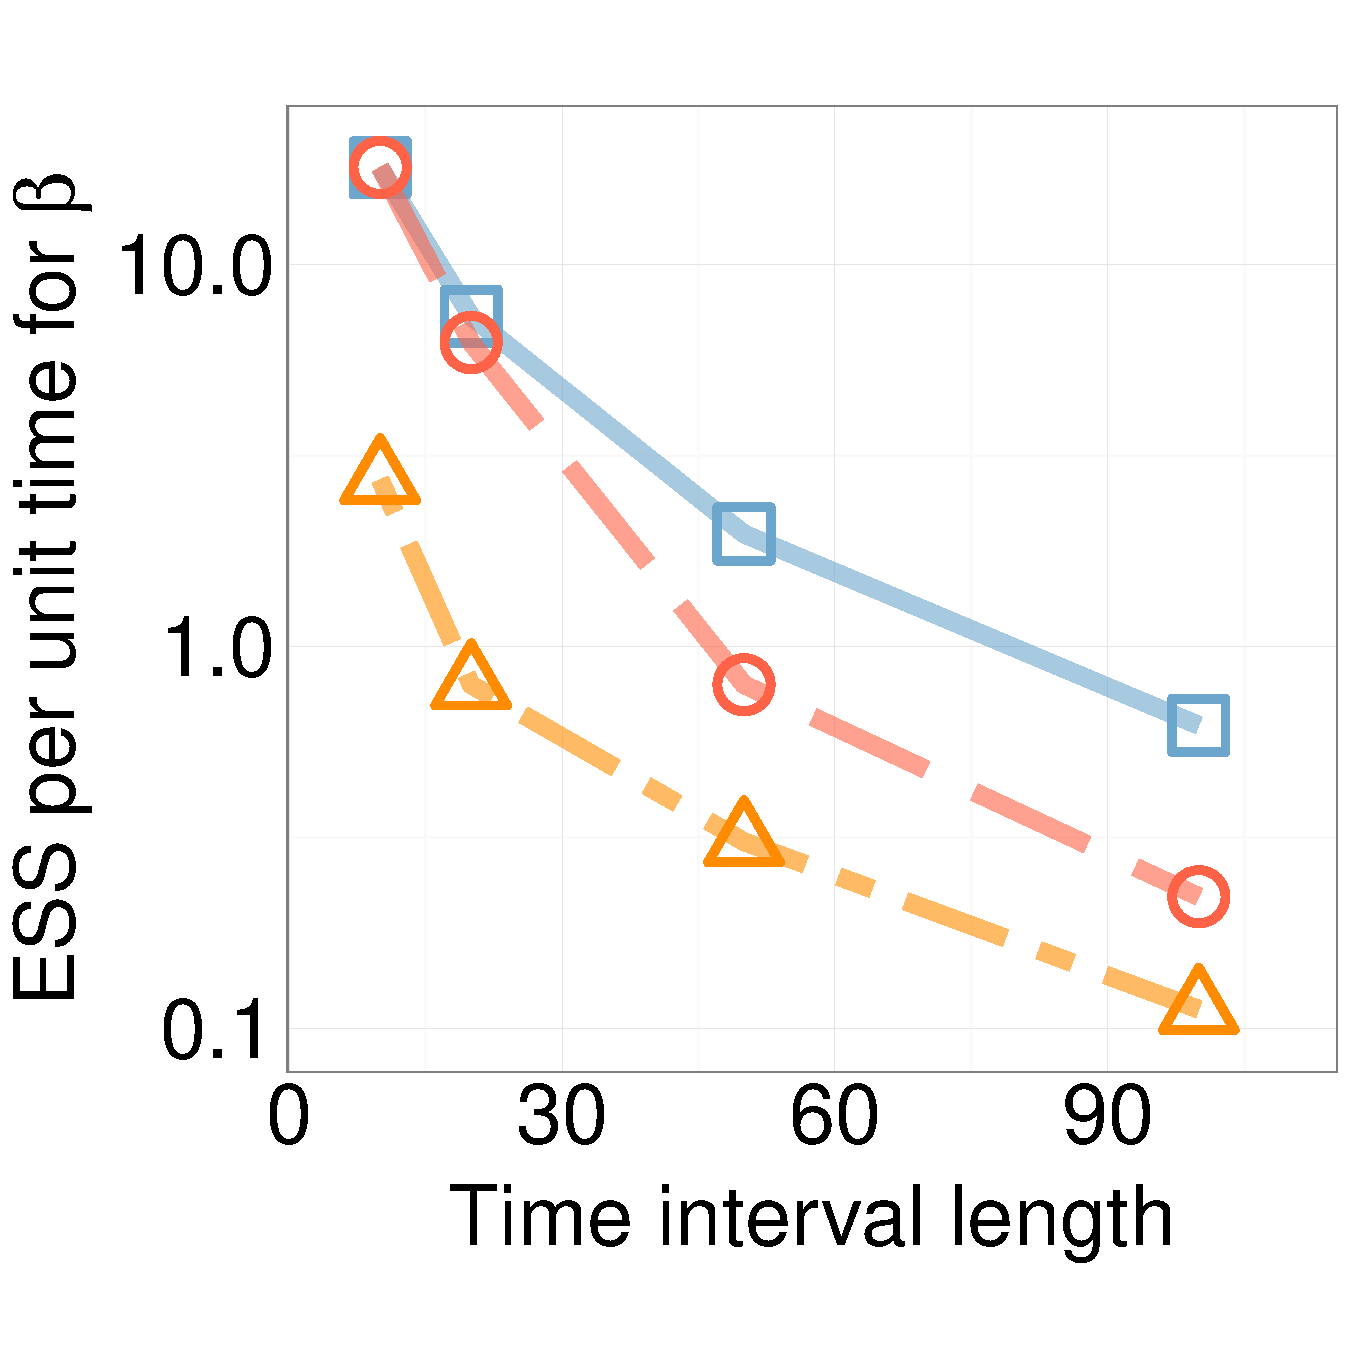
\includegraphics [width=0.99\textwidth, angle=0]{figs/new_experiment_figs/ESS_vs_t_beta.pdf}
  \end{minipage}
%    \vspace{-0.3in}
%    \caption{Time Interval vs. ESS / sec}
  \caption{Time interval vs ESS/sec for the synthetic MJP. The left two plots are for $\alpha$ and $\beta$, with the number of observations fixed; in the right two, this grows linearly with the interval length. {Blue squares, yellow triangles and red circles curves} are the symmetrized MH, \naive\ MH and Gibbs algorithm.
  }
     \label{fig:TSS}
  \end{figure}
%We generate different observations on different time intervals.
%Our observation process was a Gaussian distribution with mean equal to the 
%current state and variance equal to $1$. 
In figure~\ref{fig:TSS}, we plot ESS per unit time as the observation interval $t_{end}$ increases. 
We consider the 3-state MJP, and as before there are $19$ observations uniformly located over a time interval $(0,t_{end})$.
We consider four settings, with $t_{end}$ equal to $10, 20, 50, 100$. 
For each, we compare our symmetrized MH sampler (with $\kappa$ set to $1$) with the \naive\ MH and Gibbs samplers (with $\kappa$ set to $2$). 
While the performance of the Gibbs sampler is comparable with our symmetrized algorithm for the smallest value of $t_{end}$, its performance is considerably worse for longer time-intervals.  
This is the limitation of Gibbs sampling that motivated this work: when updating $\theta$ conditioned on the MJP trajectory, longer time intervals result in stronger coupling between MJP path and parameters, and thus poorer mixing. 
This effect disappears if we integrate out the MJP trajectory. 
The performance of the \naive\ sampler demonstrates that it is not sufficient just to integrate out the state values of the trajectory, we also have to get around the coupling between the Poisson grid and the parameters. 
Our symmetrized MH-algorithm allows this. 
%as a by-product, it also involves calculating a simpler 
%MH acceptance probability.


To the right of figure~\ref{fig:TSS}, we plot results from a similar experiment. 
Now, instead of keeping the number of measurements fixed as we increase the observation interval, we keep the observation {\em rate} fixed at one observation every unit interval of time, so that longer observation intervals have larger number of observations. 
The results are similar to the previous case: Gibbs sampling performs well for small observation intervals, with performance degrading sharply for larger intervals. 
%These two experiments illustrate the importance of integrating out the MJP path while carrying out parameter inference.

%\vspace{-.23in}
  \subsection{The Jukes and Cantor (JC69) model}~
  The Jukes and Cantor (JC69) model~\citep{jukescantor69} is a popular model of DNA nucleotide substitution.  
  We write its state space as $\{0, 1, 2, 3\}$, representing the four nucleotides $\{A, T, C, G\}$.  
  The model has a single parameter $\alpha$, representing the rate at which the system transitions between any pair of states. 
  Thus, the rate matrix $A$ is given by $A_i = -A_{i,i} = 3\alpha, A_{i, j} = \alpha,i \neq j.$
We place a Gamma$(3,2)$ prior on the parameter $\alpha$.
Figure~\ref{fig:ESS_JC}(right) compares different samplers: we see that the symmetrized MH samplers comprehensively outperforms all others.
Part of the reason why the difference is so dramatic here is because now a {\em single} paramter $\alpha \defeq \theta$ defines the transition matrix, implying a stronger coupling between MJP path and parameter. 
We point out that for Gibbs sampling, the conditional distribution over $\theta$ is conjugate to the Gamma prior. We can thus simulate directly from this distribution without any MH proposal (hence its performance remains fixed along the x-axis). 
Despite this, its performance is worse than our symmetrized algorithm.
Particle MCMC performs worse than all the algorithms, and we do not include it in our plots.
%  \begin{figure}%[H]
%  \begin{minipage}[!hp]{0.7\linewidth}
%    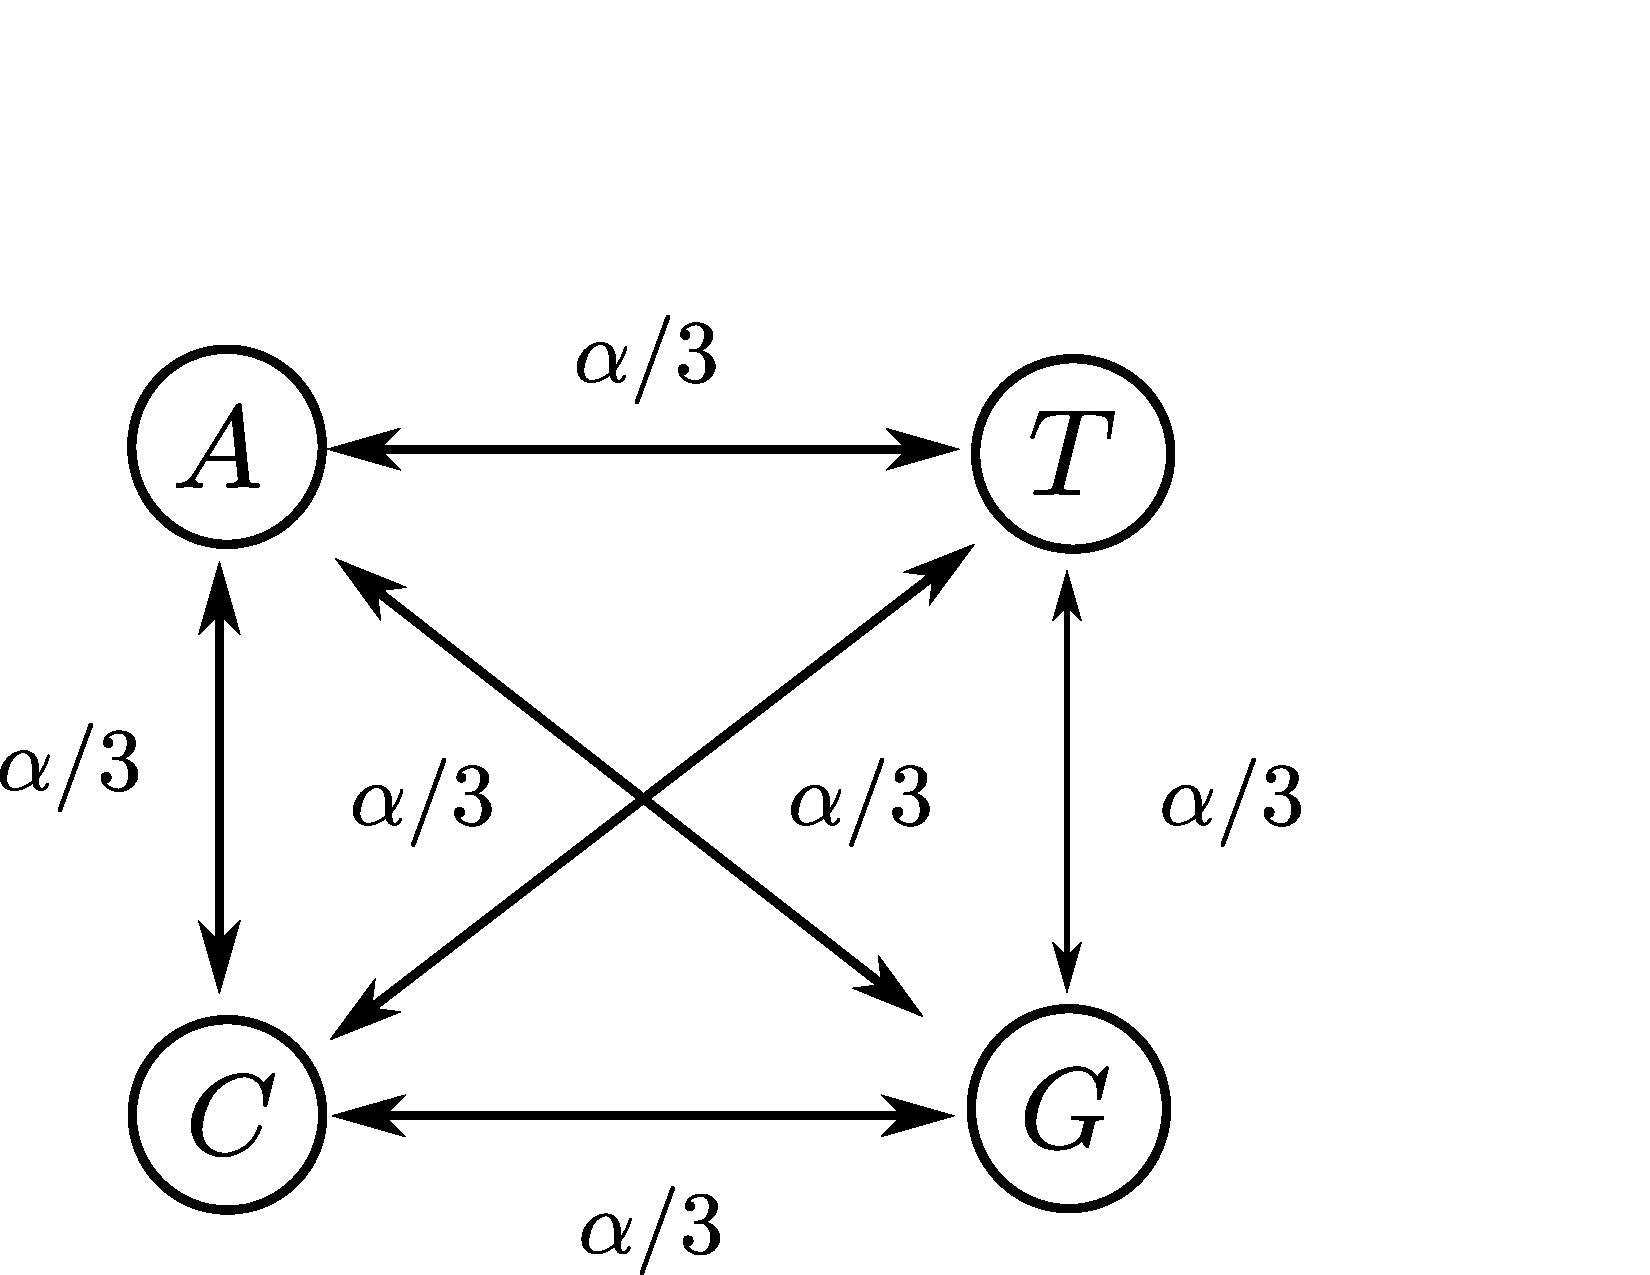
\includegraphics[width=0.49\textwidth, angle=0]{figs/jc_model.pdf} 
 %   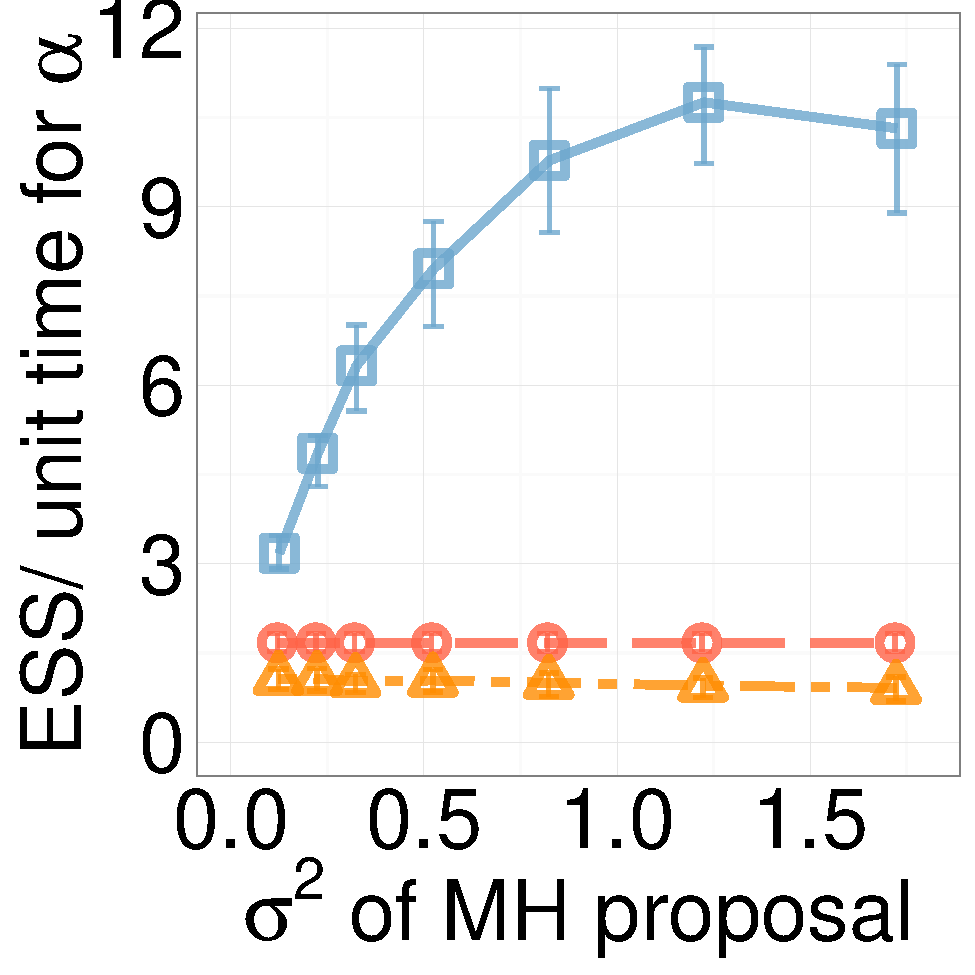
\includegraphics[width=0.49\textwidth, angle=0]{figs/new_experiment_figs/jc_alpha_k2.pdf}
 % \end{minipage}
 % \begin{minipage}[!hp]{0.28\linewidth}
 % \caption{(a) Jukes-Cantor (JC69) model, (b)
  %  ESS/sec for the JC69 Model. Red, yellow and blue curves are the 
   %   symmetrized MH, \naive\ MH and Gibbs algorithm. }
   %  \label{fig:ESS_JC}
  %\end{minipage}
 %\end{figure}

   \begin{figure}%[H]
  \begin{minipage}[!hp]{0.24\linewidth}
	\centering
    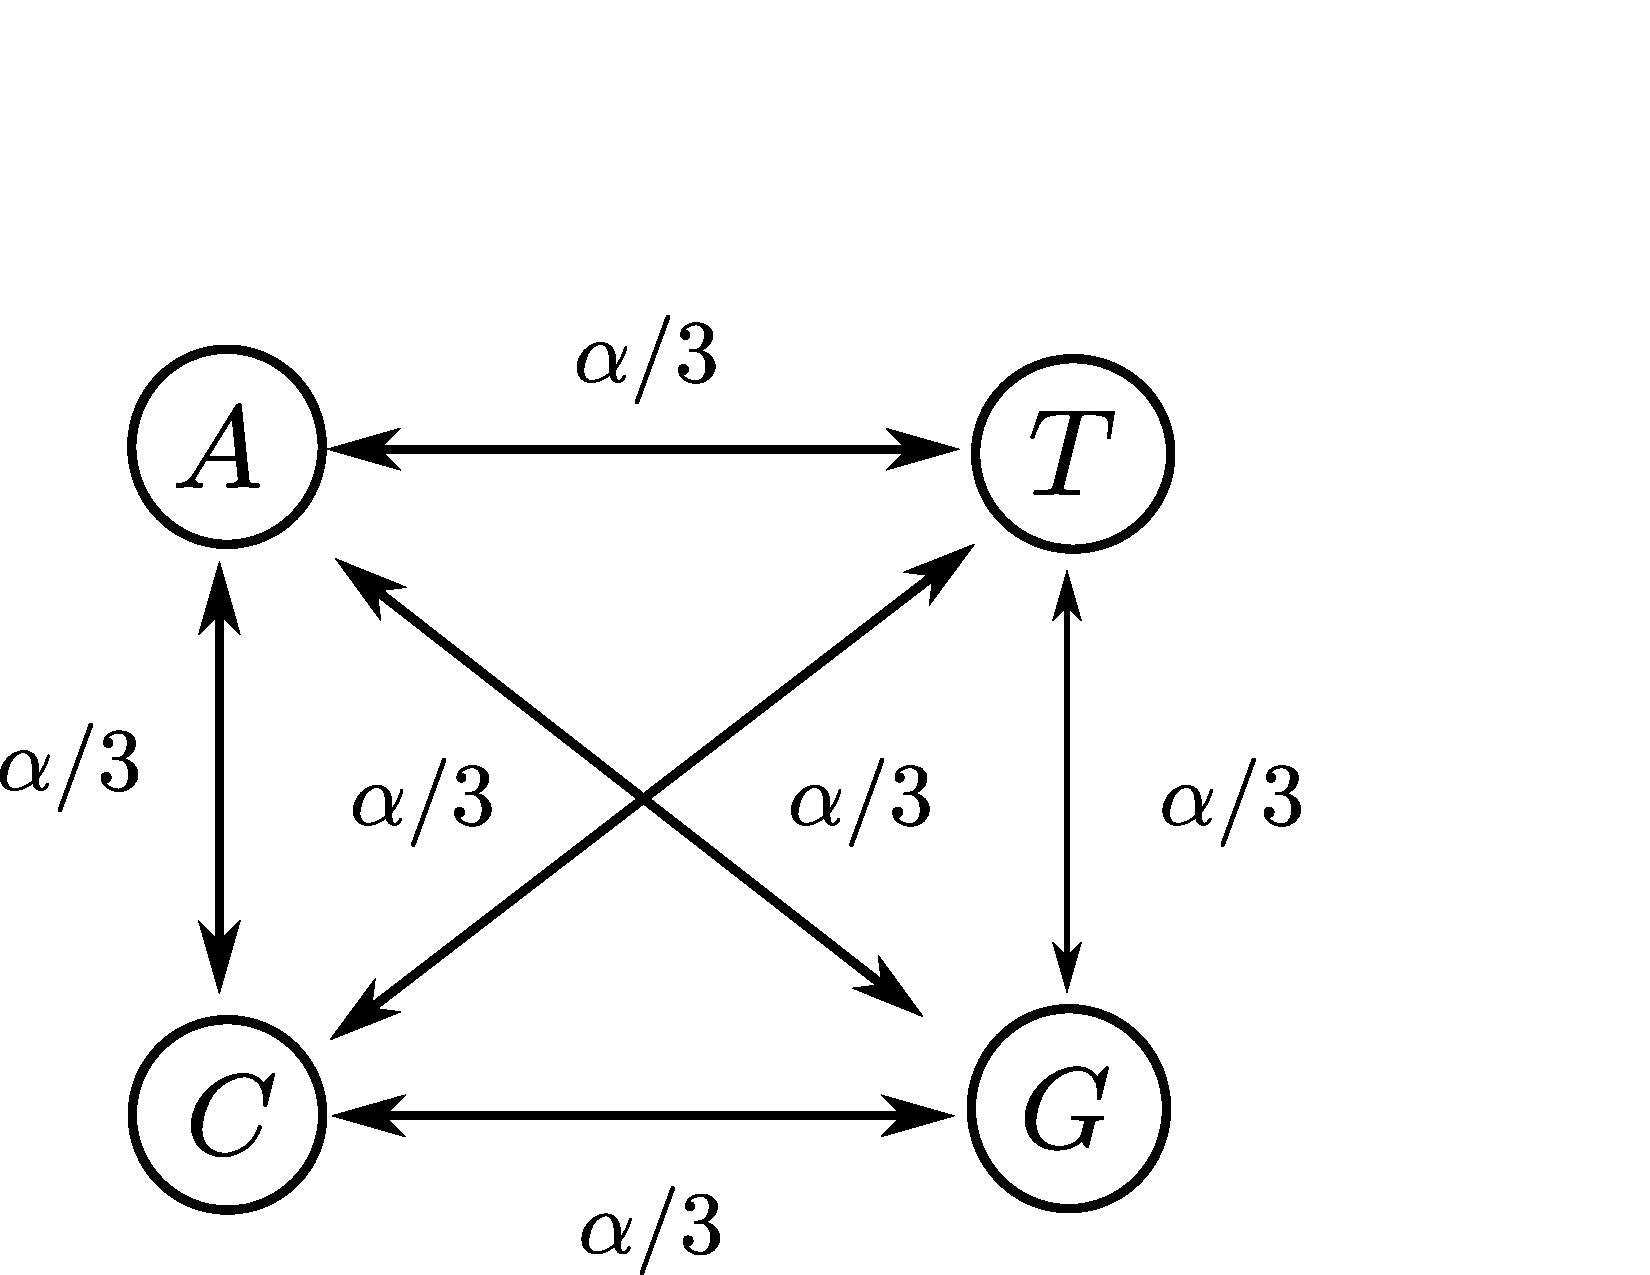
\includegraphics[width=0.99\textwidth, angle=0]{figs/jc_model.pdf} 
	\end{minipage}
	  \begin{minipage}[!hp]{0.24\linewidth}
	\centering
    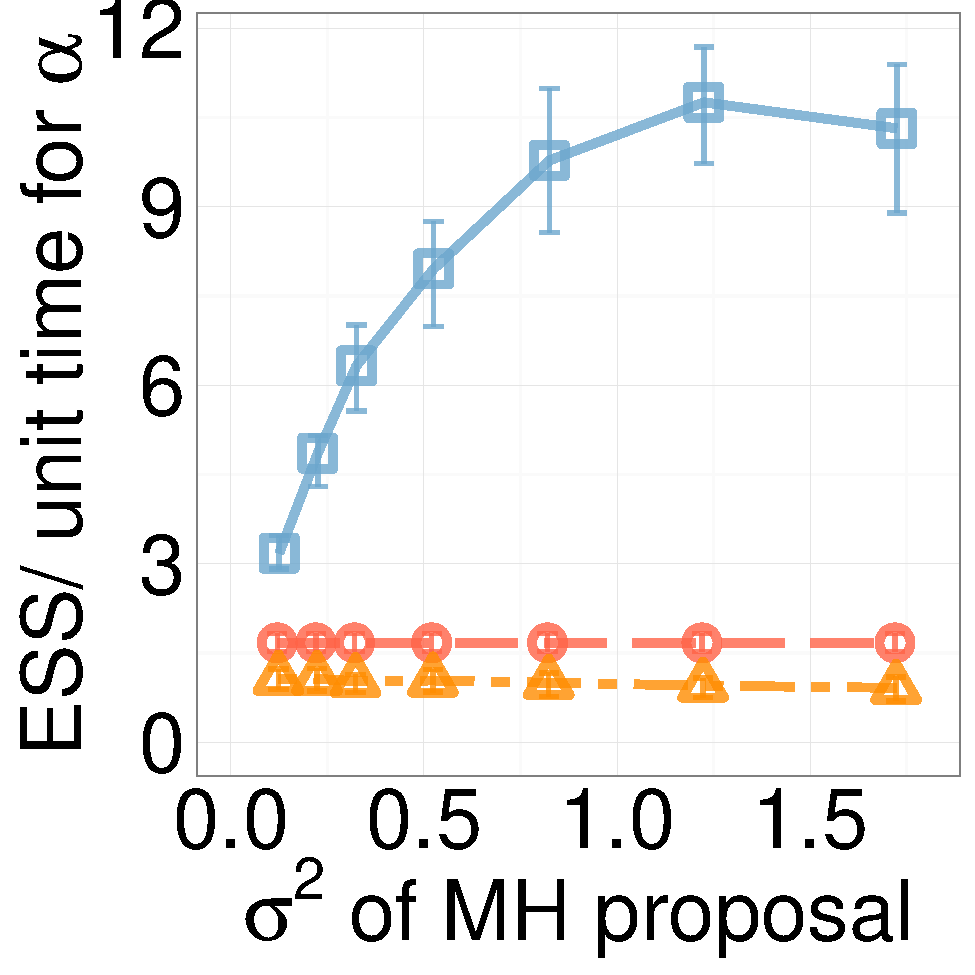
\includegraphics[width=0.99\textwidth, angle=0]{figs/new_experiment_figs/jc_alpha_k2.pdf}
  \end{minipage}
  \begin{minipage}[!hp]{0.24\linewidth}
	\centering
    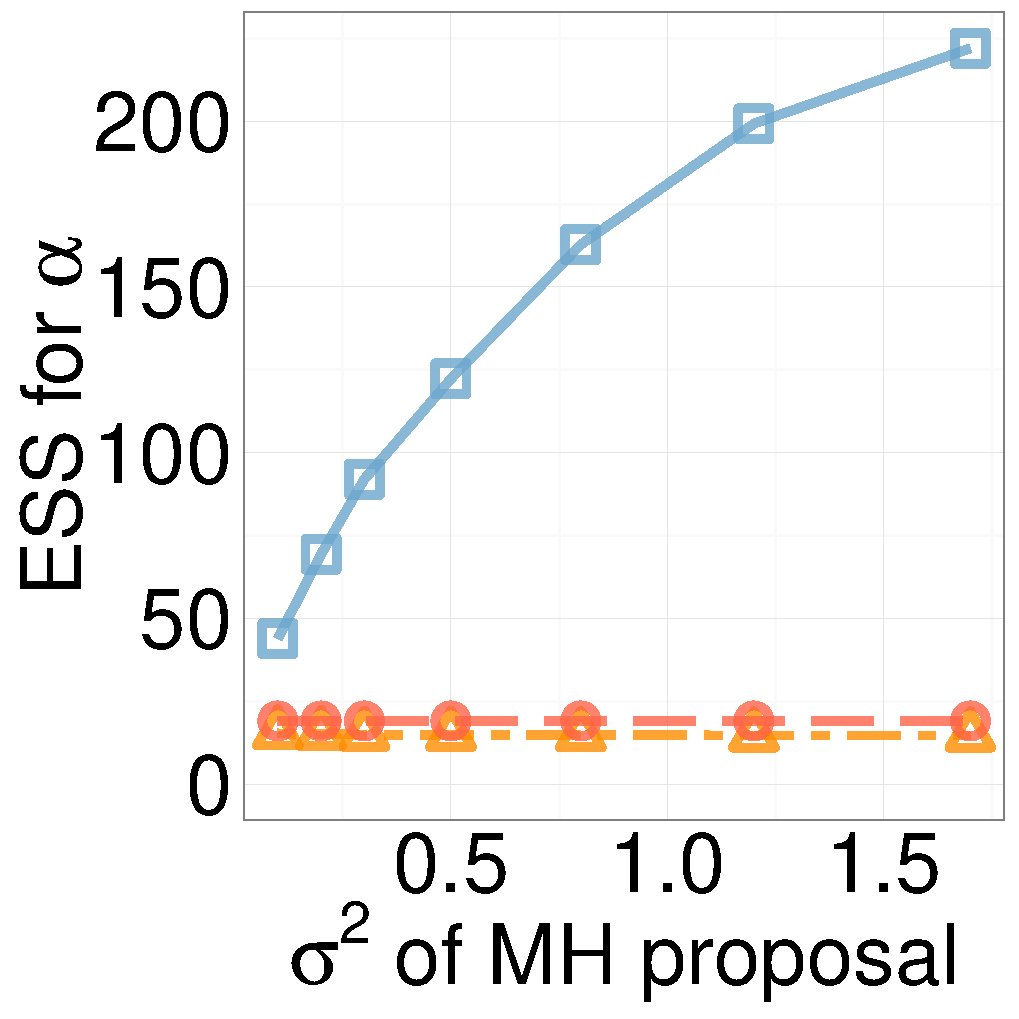
\includegraphics[width=0.99\textwidth, angle=0]{figs/ess/JCalpha_k2.pdf}
\end{minipage}
  \begin{minipage}[!hp]{0.24\linewidth}
	\centering
    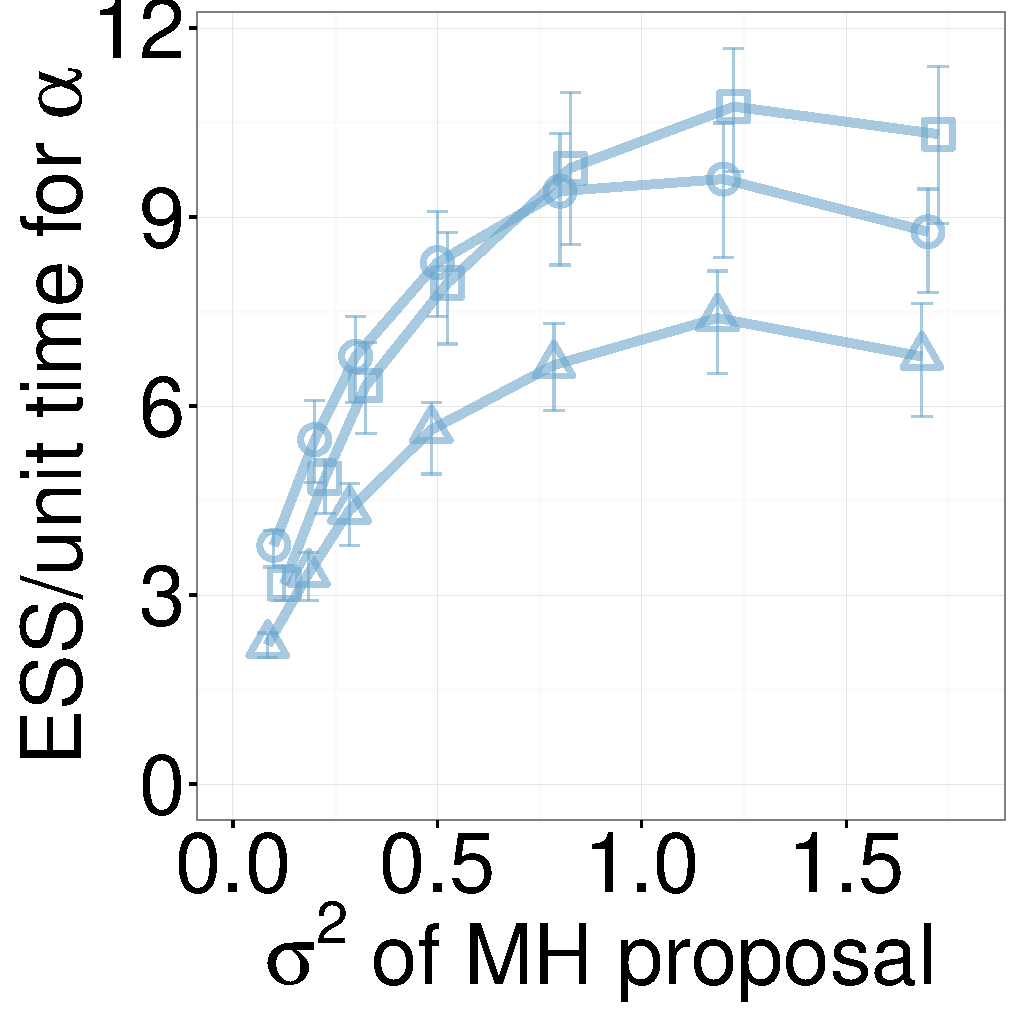
\includegraphics[width=0.99\textwidth, angle=0]{figs/new_whole_exp_figs/mh_jc_alpha.pdf}
\end{minipage}
%  \begin{minipage}[!hp]{0.28\linewidth}
  \caption{The leftmost panel is the Jukes-Cantor (JC69) model. The next two panels from left to right are ESS/sec and raw ESS per 1000 samples for this. 
    Blue squares, yellow triangles and red circles are the symmetrized MH, \naive\ MH and Gibbs algorithm.
    The rightmost panel looks at different settings of the symmetrized MH algorithm, with squares, circles and triangles corresponding to 
$\Omega(\theta,\vartheta)$ set to $(\max_s A_s(\theta) + \max_s A_s(\vartheta))$, $\max(\max_s A_s(\theta), \max_s A_s(\vartheta))$ and  $1.5(\max_s A_s(\theta) + \max_s A_s(\vartheta))$.
     \label{fig:ESS_JC}
   }
 % \end{minipage}
 \end{figure}

  \begin{figure}[H]
  \centering

  \begin{minipage}[!hp]{0.99\linewidth}
  	\centering
    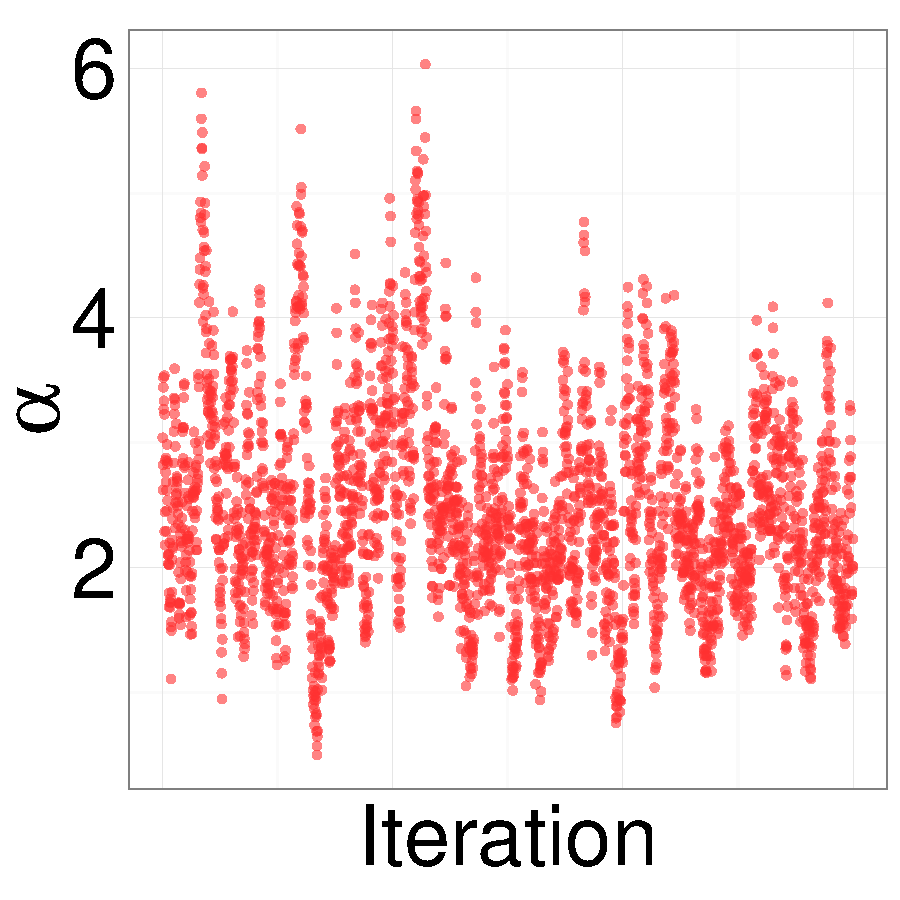
\includegraphics [width=0.24\textwidth, angle=0]{figs/JC_ks/jc_traceGBS_44_05_3_.pdf}
    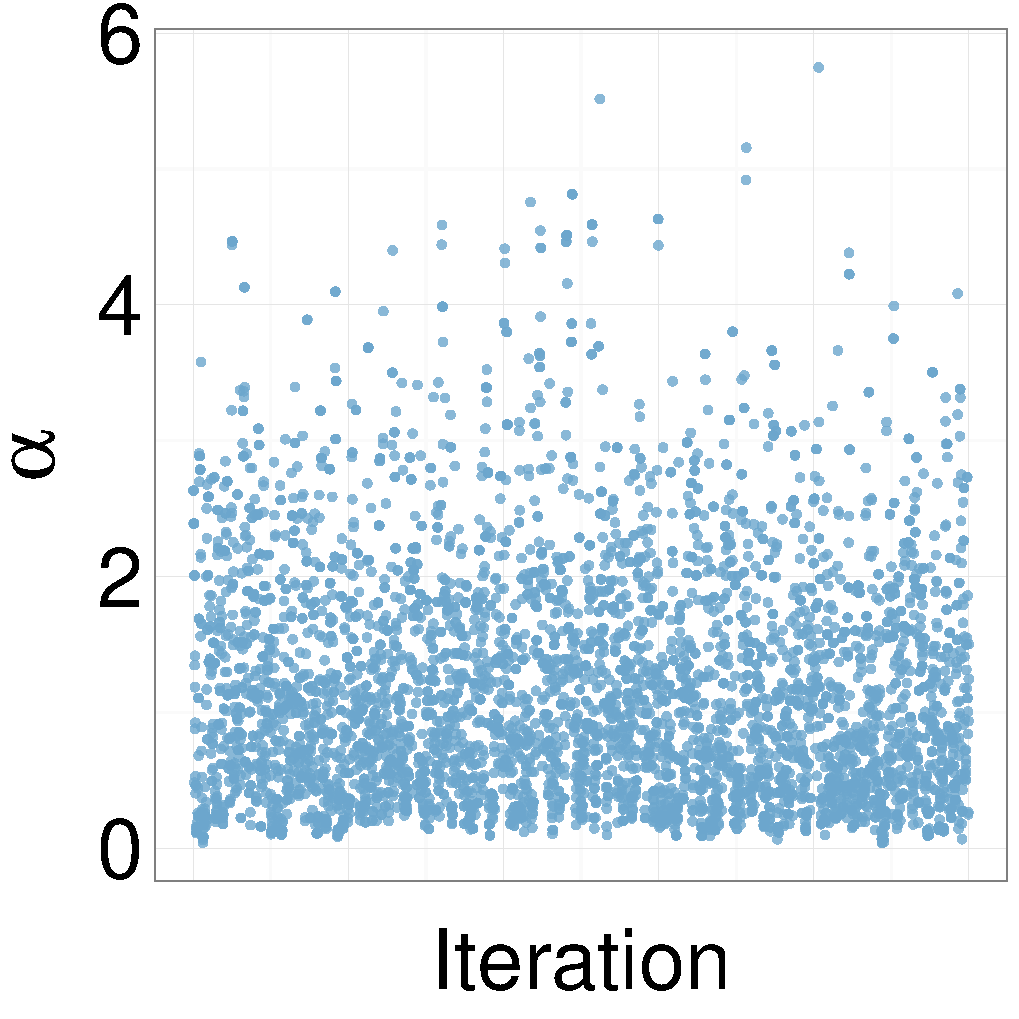
\includegraphics [width=0.24\textwidth, angle=0]{figs/JC_ks/jc_traceMH_44_05_3_.pdf}
    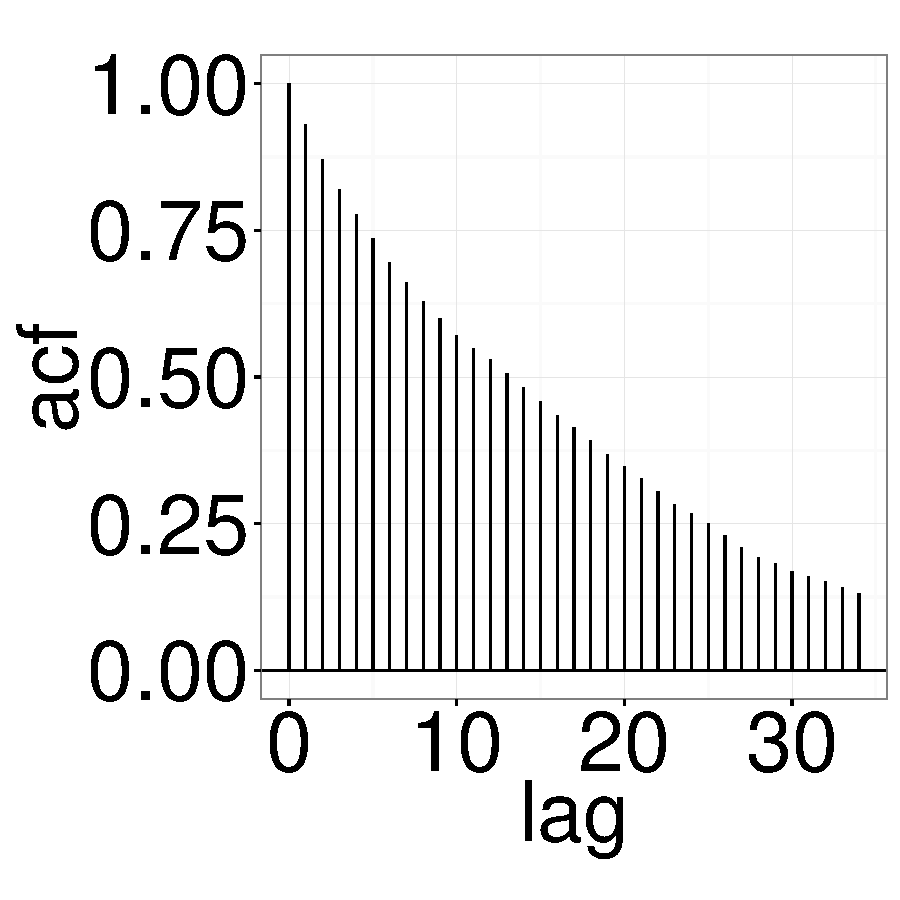
\includegraphics [width=0.24\textwidth, angle=0]{figs/JC_ks/jc_gbsacf_44_05_3_.pdf}
    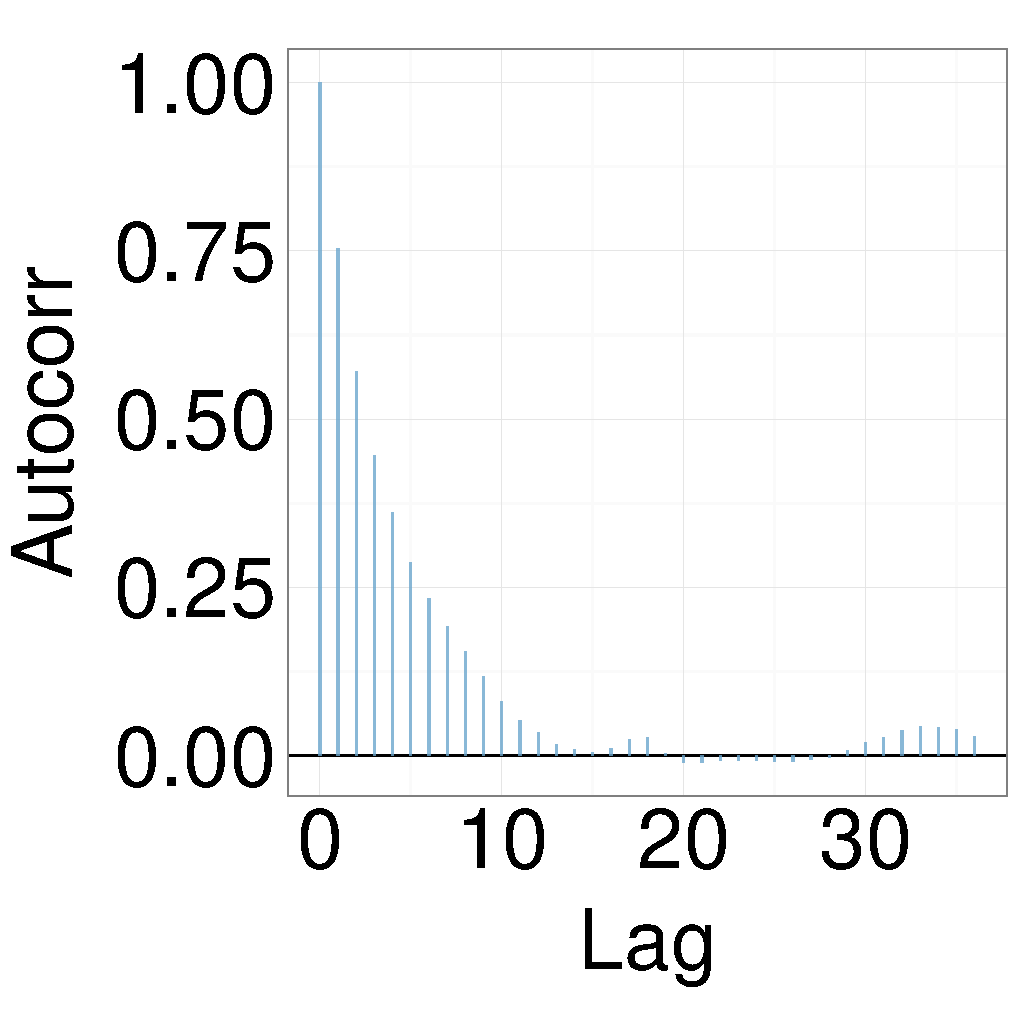
\includegraphics [width=0.24\textwidth, angle=0]{figs/JC_ks/jc_mhacf_44_05_3_.pdf}
  \end{minipage}
%  \begin{minipage}[!hp]{0.99\linewidth}
    \caption{Trace and autocorrelation plots of $\alpha$ for the JC69 model. Left two panels are for Gibbs and the right two for the symmetrized MH algorithm.}
    \label{fig:ACC_JC_m}
%  \end{minipage}
  \end{figure}
  Figure~\ref{fig:ACC_JC_m} plots MCMC diagnostics for the Gibbs and symmetrized MH sampler, again the latter outperforms the former. 
  Both agree on the posterior $P(\alpha|X)$ (figure~\ref{fig:jc_model_vs_t}(a)), with a two sample Kolmogorov-Smirnov test giving a p-value of $0.97$. 
  Figure~\ref{fig:jc_model_vs_t}(b) plots the average MH acceptance probabilities for the \naive\ and symmetrized MH samplers for different settings of the proposal distribution, again we see that the former has lower acceptance rates because of the $P(W|\theta)$ grids.
%  \begin{figure}%[H]
%  \centering
%  \begin{minipage}[!hp]{0.58\linewidth}
%  \centering
 %   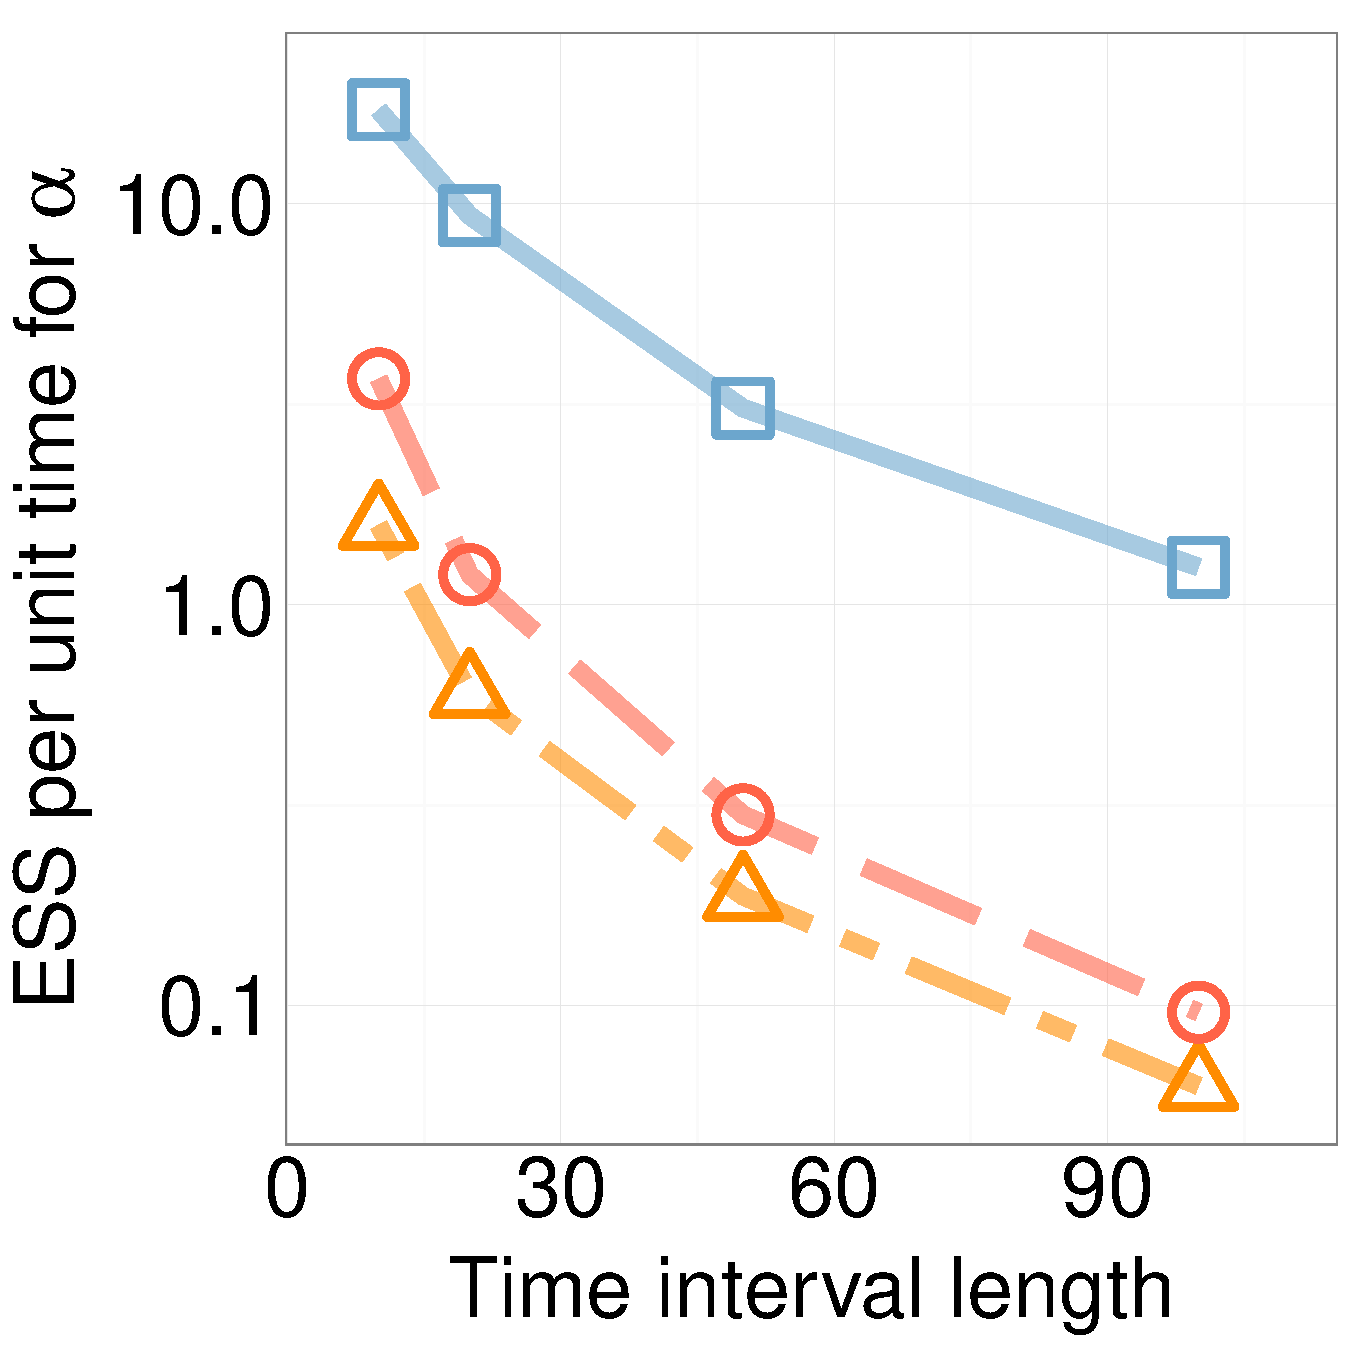
\includegraphics [width=0.49\textwidth, angle=0]{figs/new_experiment_figs/ESS_vs_t_alpha_JC.pdf}
  %  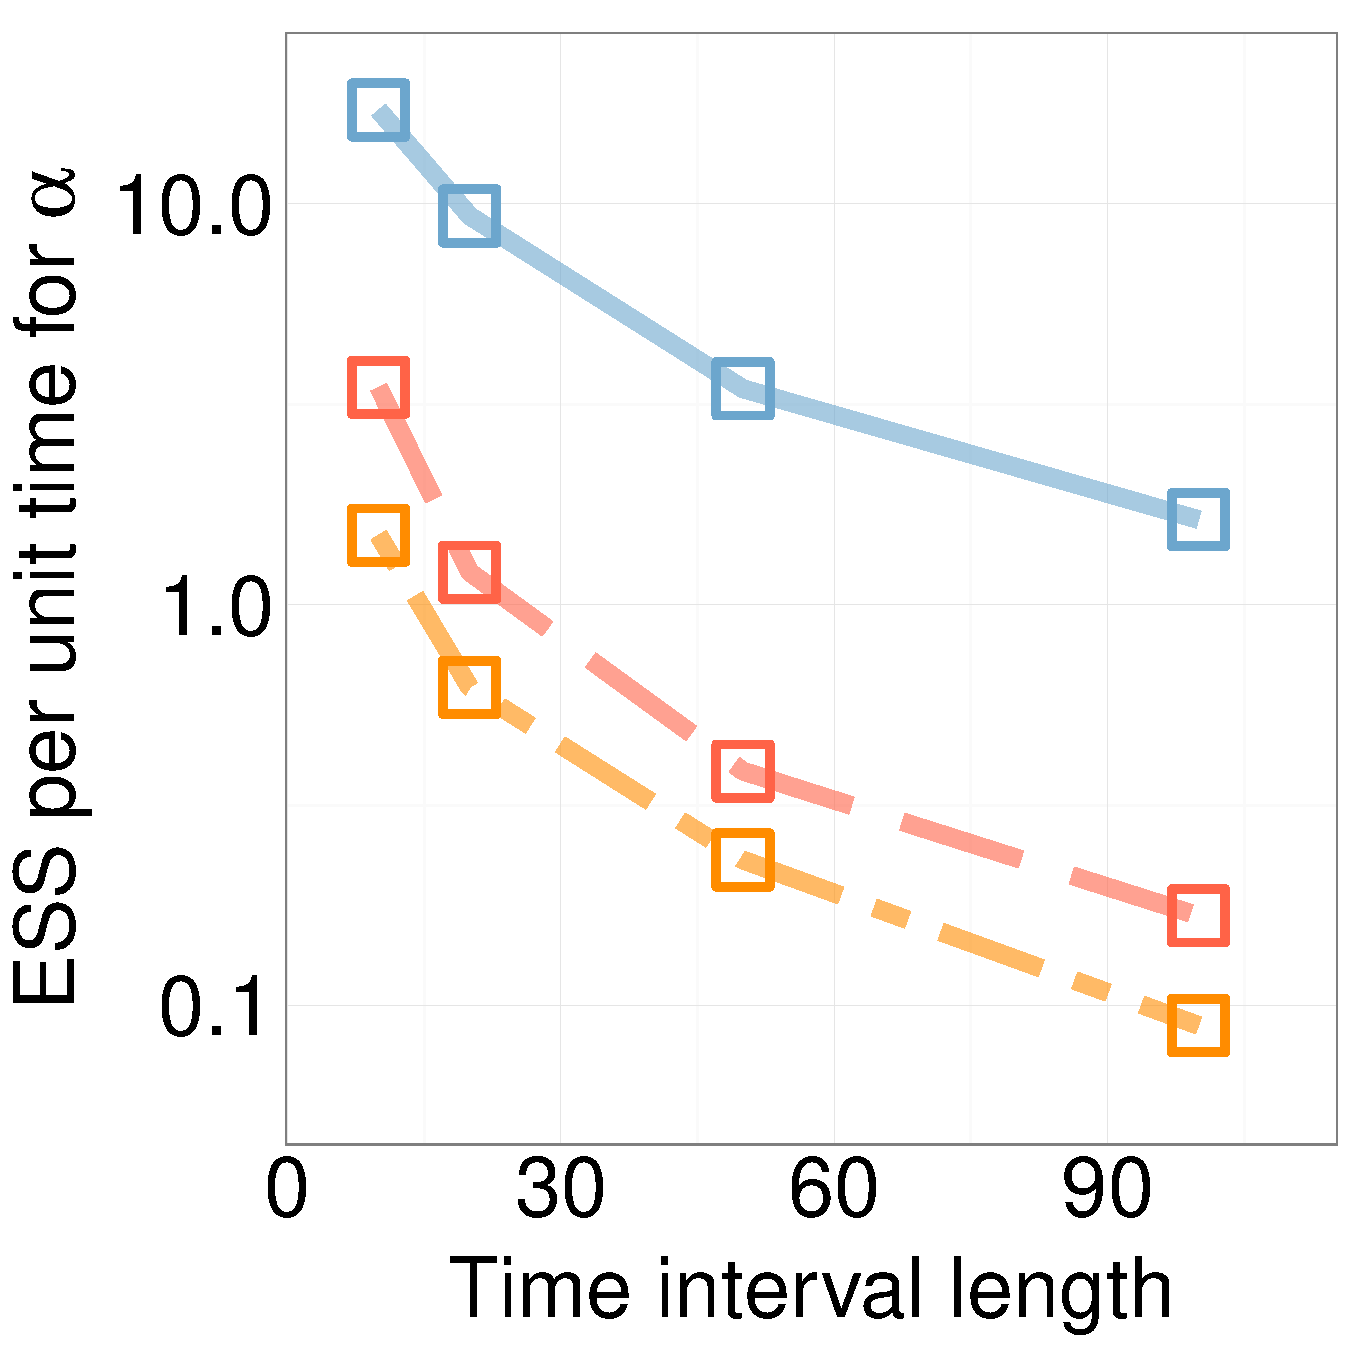
\includegraphics [width=0.49\textwidth, angle=0]{figs/new_experiment_figs/ESS_vs_t_alpha_fixobservation_JC.pdf}
  %\end{minipage}
  %\begin{minipage}[!hp]{0.01\linewidth}
  %\end{minipage}
  %\begin{minipage}[!hp]{0.4\linewidth}
   % \caption{Time Interval vs.\ ESS/sec for JC model. Number of observations is fixed (left), and grows linearly with interval (right). Squares, circles and triangles are the symmetrized MH, \naive\ MH and Gibbs. }
%	\label{fig:jc_model_vs_t}
 % \end{minipage}
%  \end{figure}
  \begin{figure}%[H]
  \centering
  \begin{minipage}[!hp]{0.99\linewidth}
  \centering
    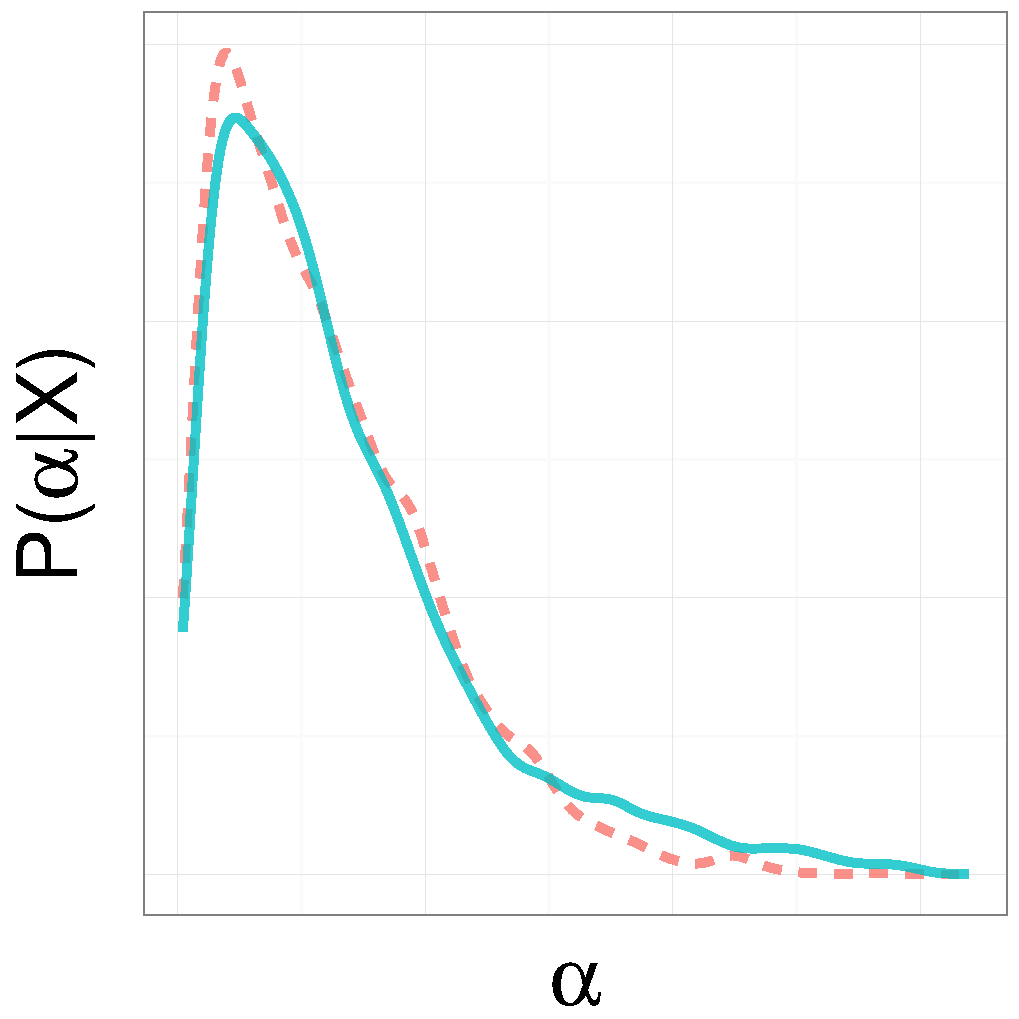
\includegraphics [width=0.24\textwidth, angle=0]{figs/JC_ks/jc_hist_44_05_3_.pdf}
    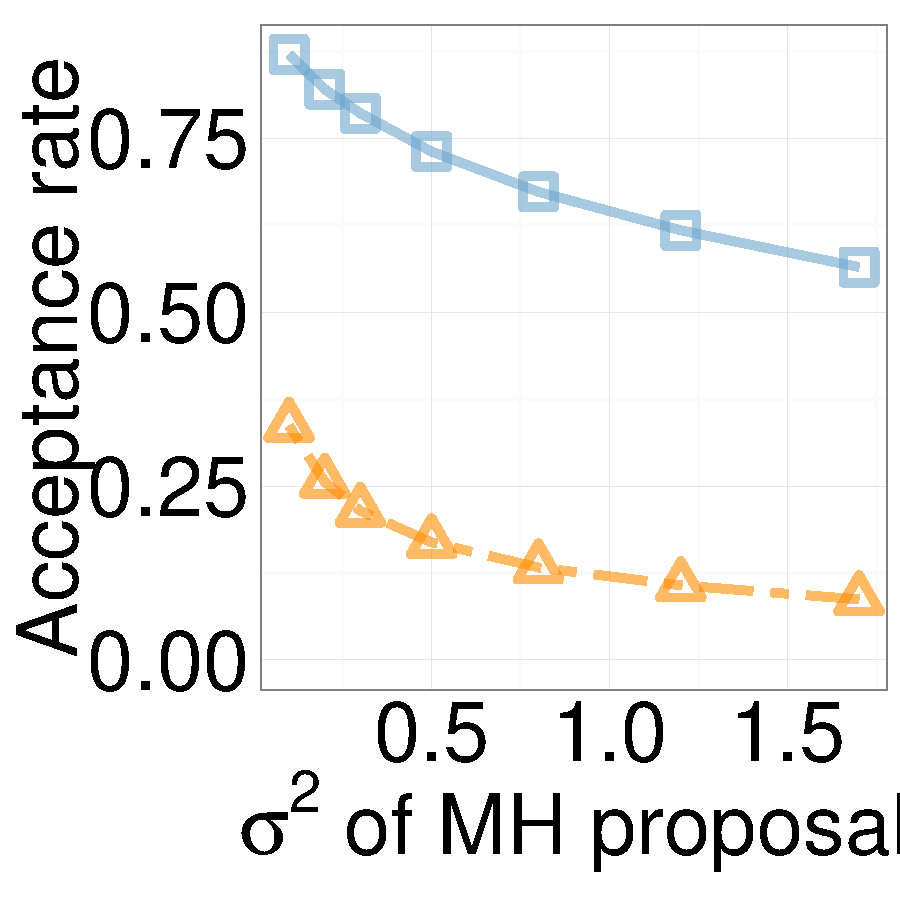
\includegraphics [width=0.24\textwidth, angle=0]{figs/acc/JCalpha_k2.pdf}
    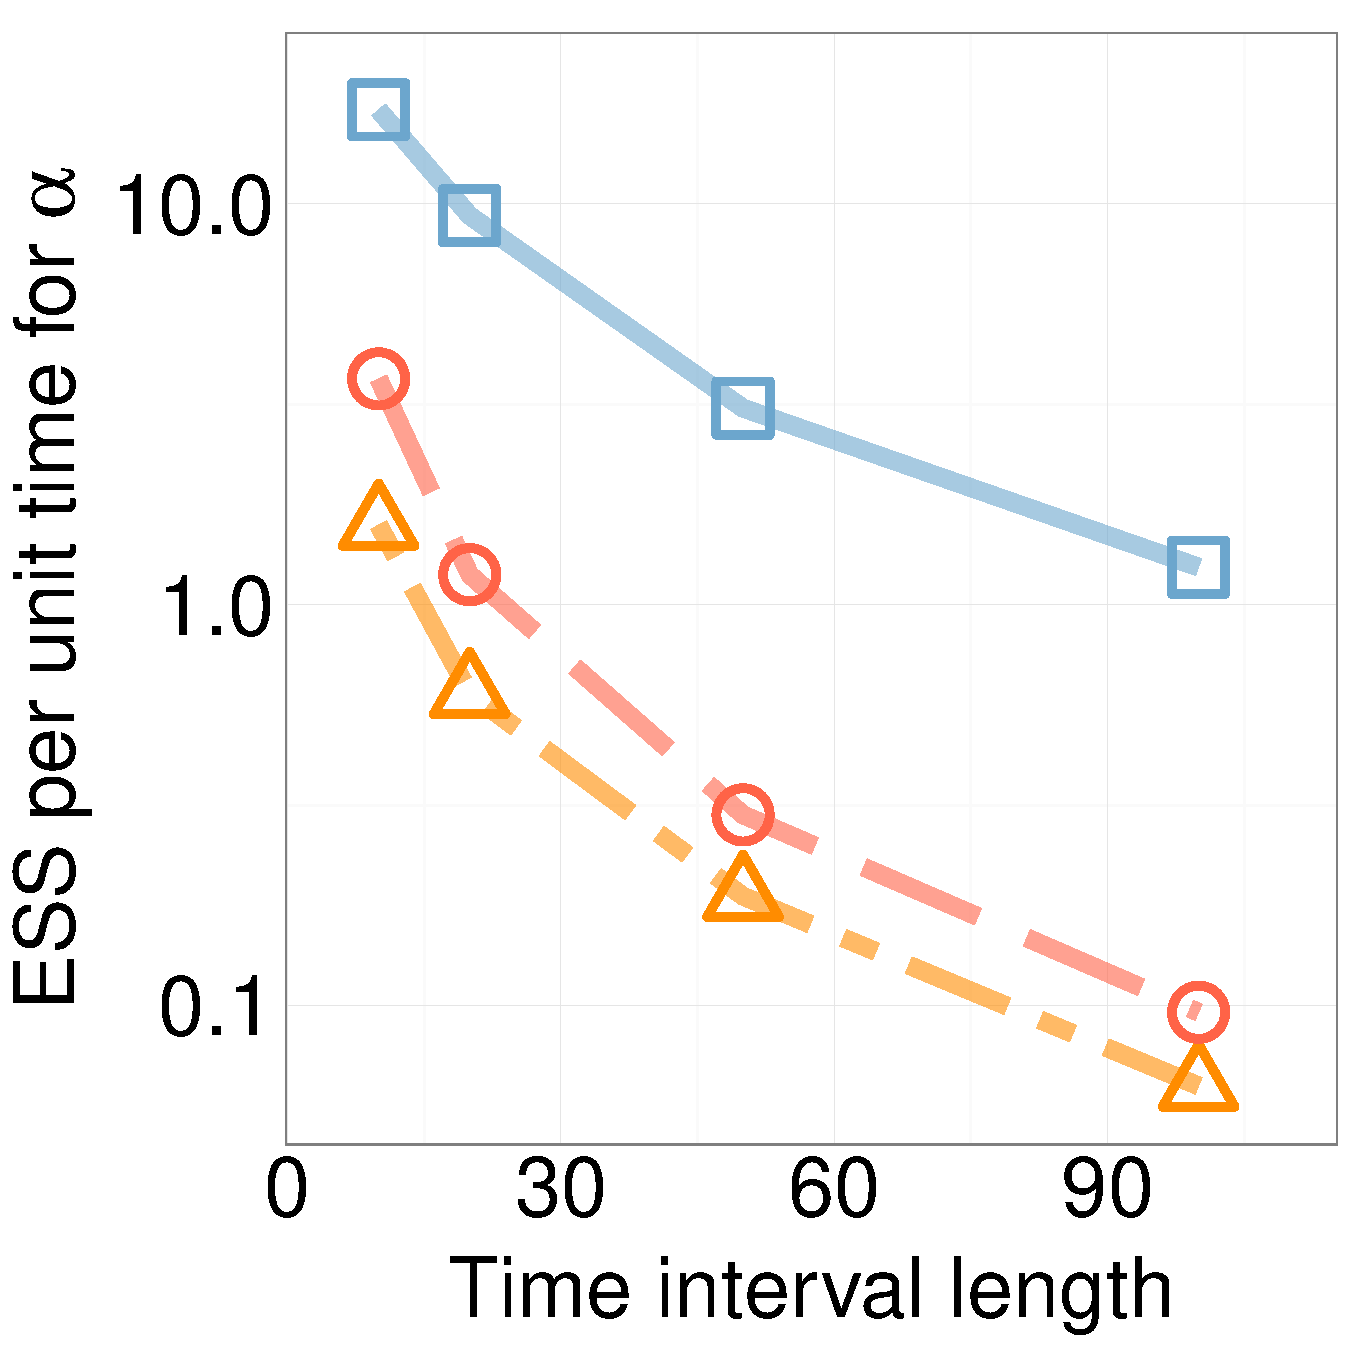
\includegraphics [width=0.24\textwidth, angle=0]{figs/new_experiment_figs/ESS_vs_t_alpha_JC.pdf}
    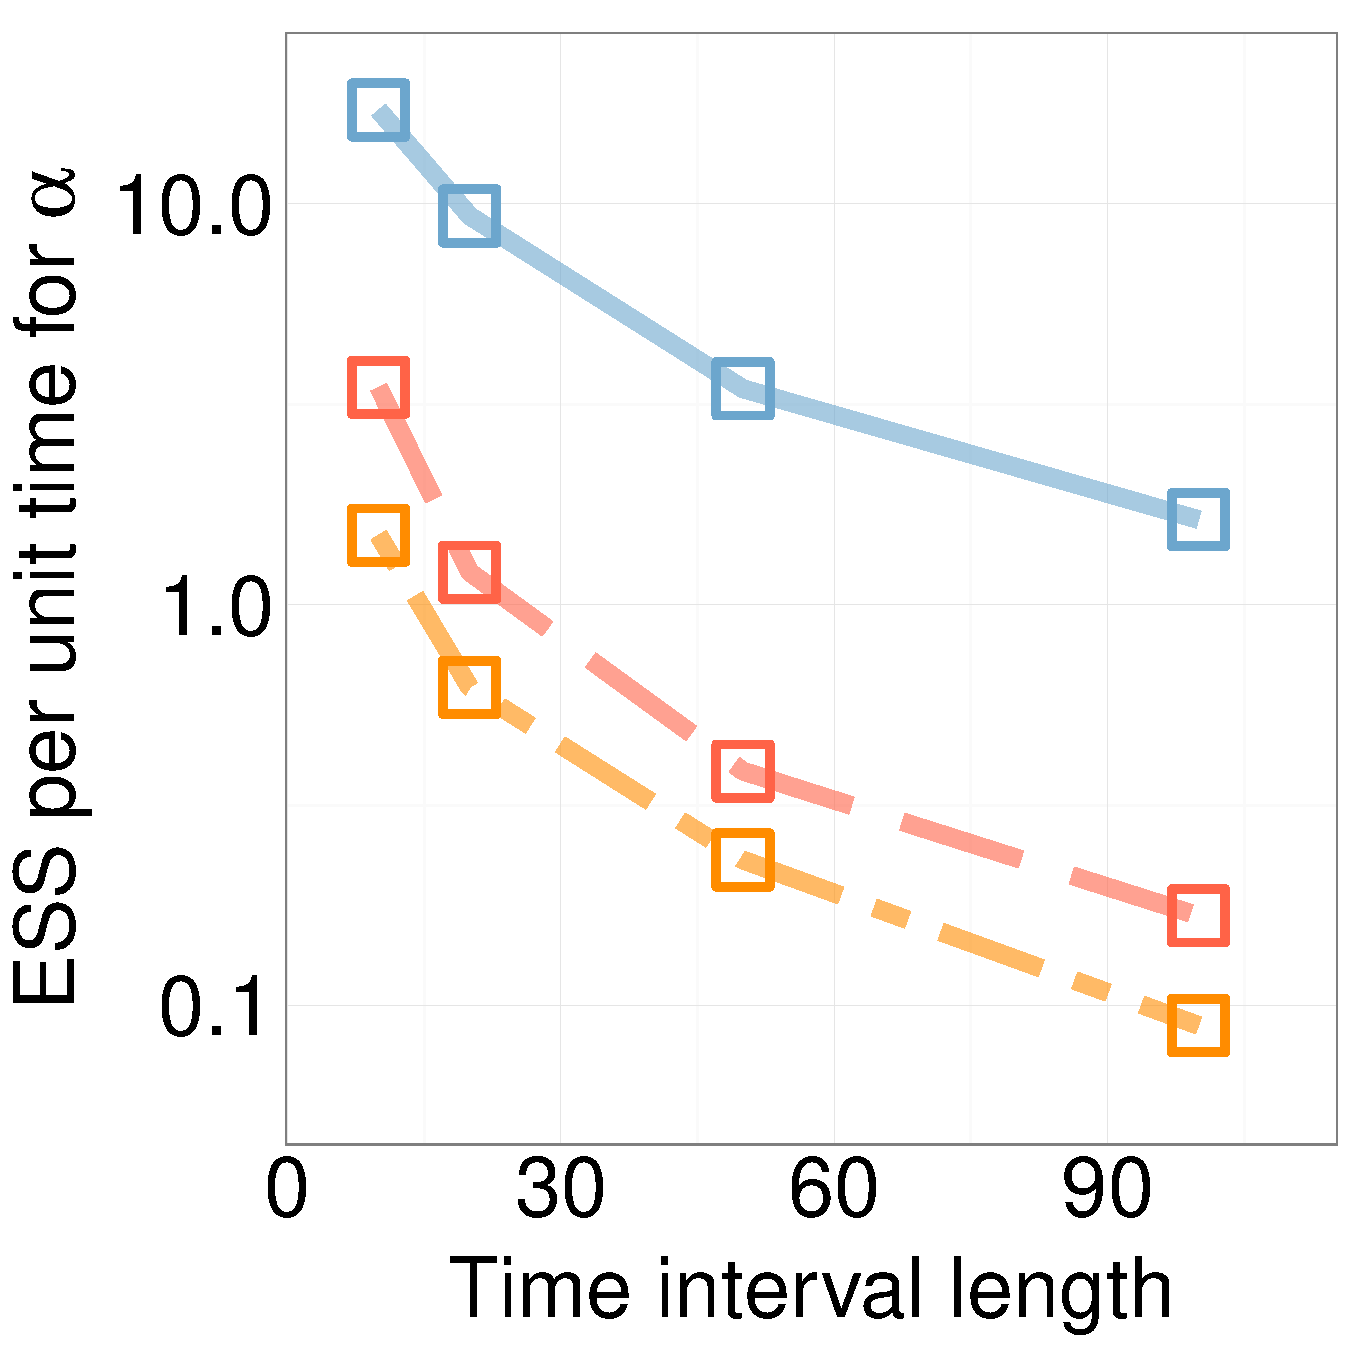
\includegraphics [width=0.24\textwidth, angle=0]{figs/new_experiment_figs/ESS_vs_t_alpha_fixobservation_JC.pdf}
  \end{minipage}

%  \begin{minipage}[!hp]{0.24\linewidth}
  \caption{(a) Posterior $P(\alpha|X)$ in the JC69 model for Gibbs (dashed) and symmetrized MH (continuous). (b) MH acceptance rates for \naive\  and symmetrized MH. (c) and (d):
  ESS/sec against $t_{end}$ for $\kappa=2$ with: (c) number of observations fixed, and (d) observation rate fixed. {Squares, triangles and circles} are symmetrized MH, \naive\ MH and Gibbs. }
	\label{fig:jc_model_vs_t}
%  \end{minipage}
%  \vspace{-.4in}
  \end{figure}
  Figure~\ref{fig:jc_model_vs_t} (c) and (d) plot the ESS per unit time for the
  different samplers as $t_{end}$ increases. 
  The left plot keeps the number of observations fixed, while the right keepss the observation rate fixed. 
Once again we see that our proposed algorithm
1) performs best over all interval lengths, and 2) suffers a performance
degradation with interval length that is much milder than the other algorithms.
%$$p(\alpha) = \frac{\lambda^\mu}{\Gamma(\mu)}\alpha^{\mu -1}e^{-\lambda \alpha} $$.
%Then we can get the posterior distribution $$f(\alpha | s_0,S,T)$$ as follows.
%$$ f(\alpha| s_0,S,T) \propto \exp(-(\lambda + 3(t_{end} - t_{start}))\alpha) \alpha^{\mu + N -1} .$$
%$\alpha | s_0,S,T$ is following $Gamma(\mu+ N,\lambda + 3(t_{end} - t_{start}))$\\

%  \vspace{-.25in}
\subsection{An immigration model with finite capacity}\label{sec:immig}~
%  \begin{figure}%[b]
 % \centering
  %\begin{minipage}[hp]{0.69\linewidth}
%    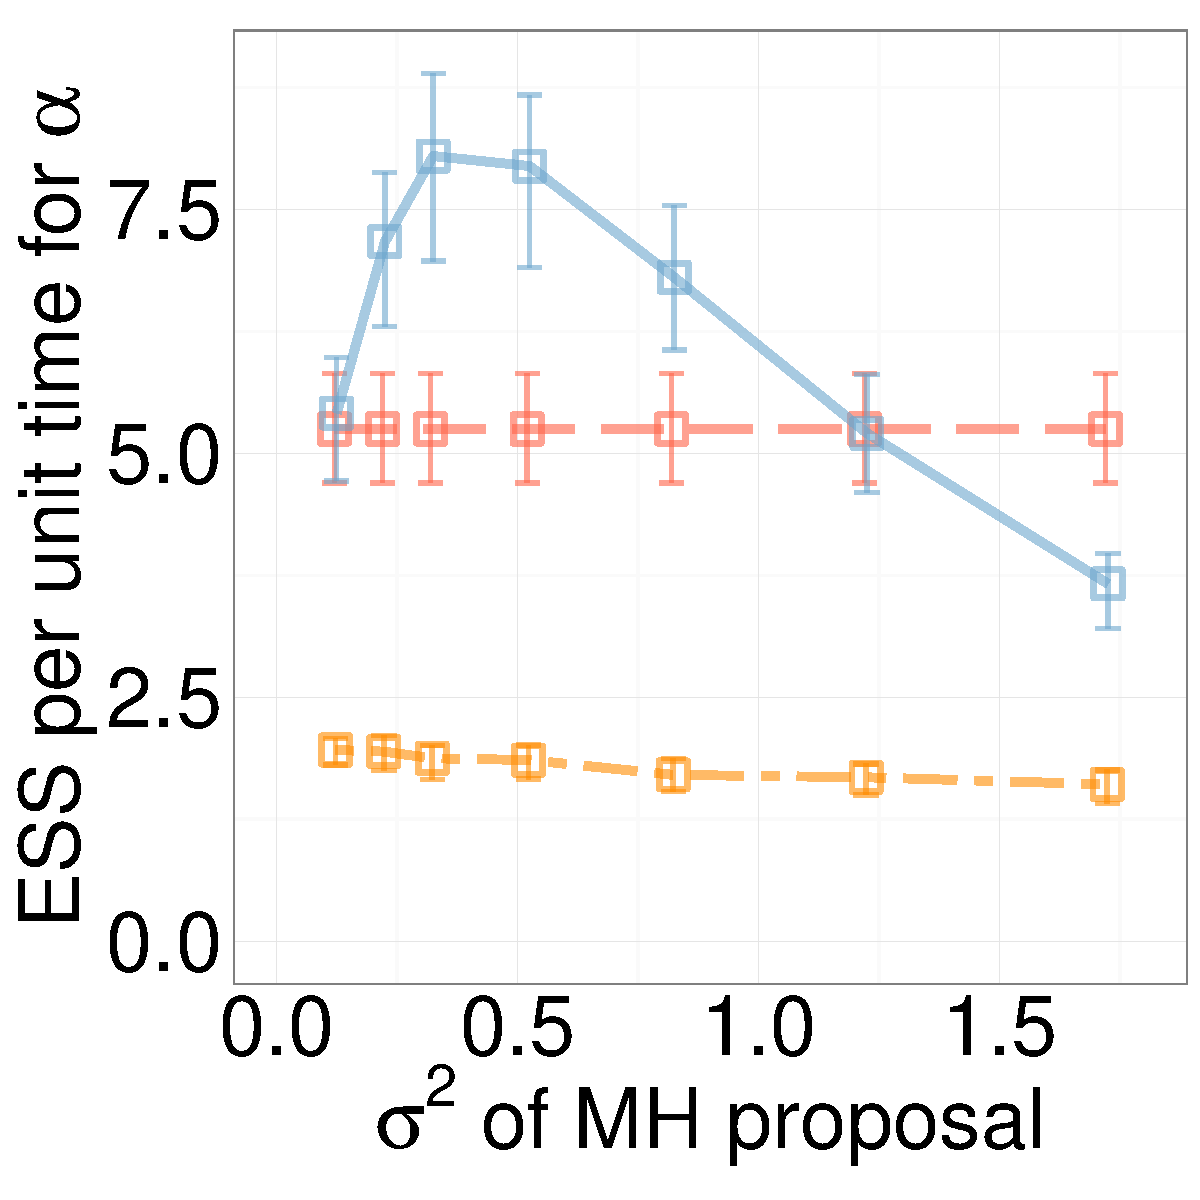
\includegraphics [width=0.49\textwidth, angle=0]{figs/new_experiment_figs/q_alpha_dim3_k2.pdf}
 %   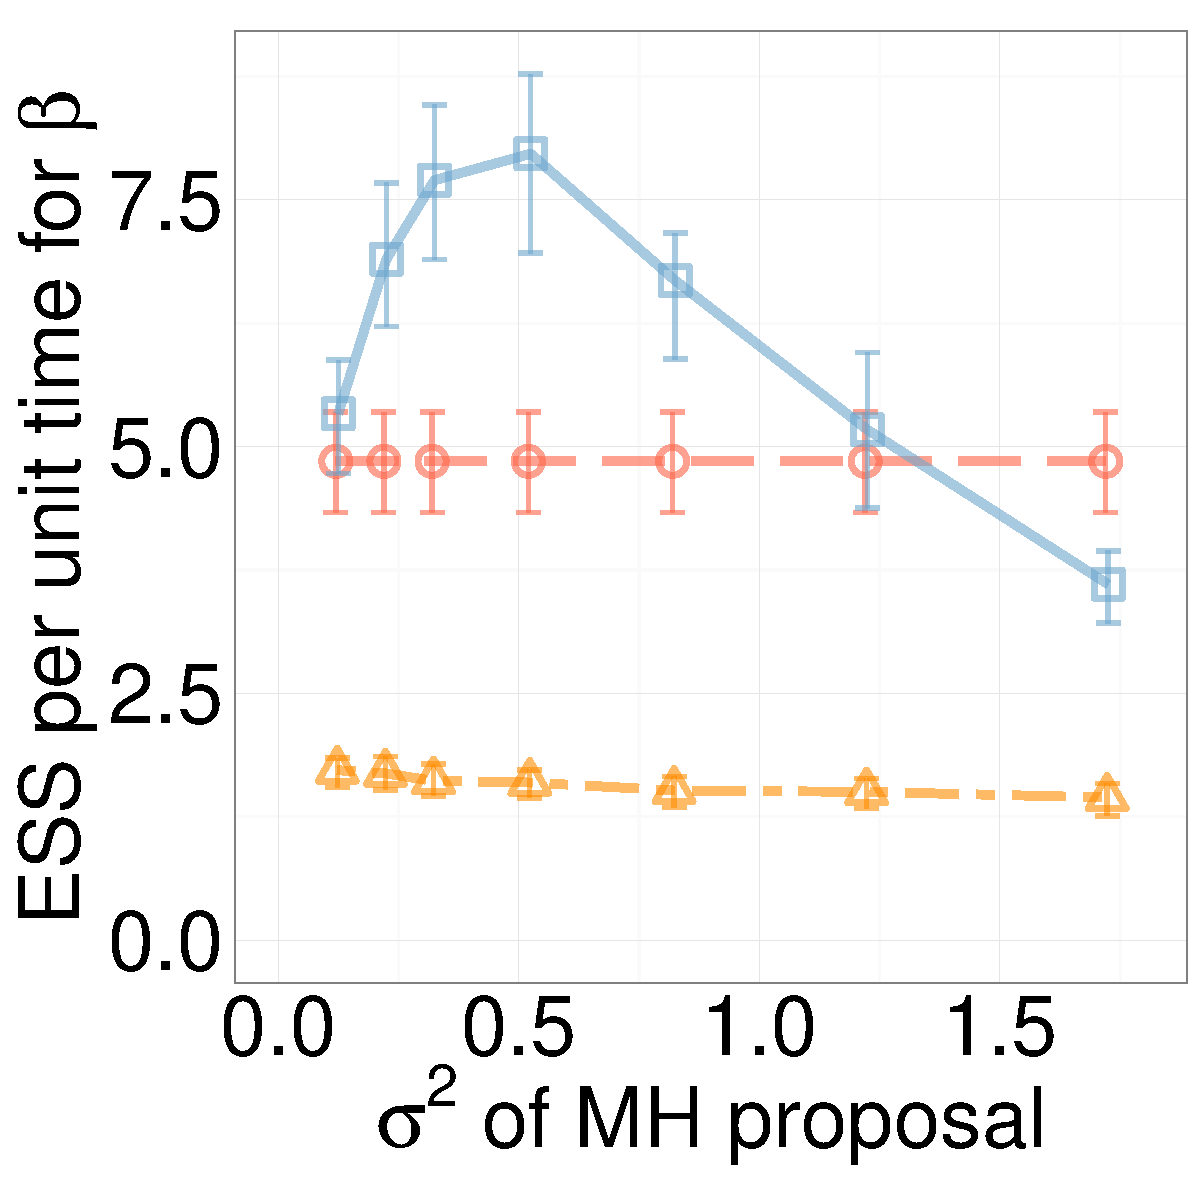
\includegraphics [width=0.49\textwidth, angle=0]{figs/new_experiment_figs/q_beta_dim3_k2.pdf}
  %  \vspace{-.1 in}
  %\centering
   % 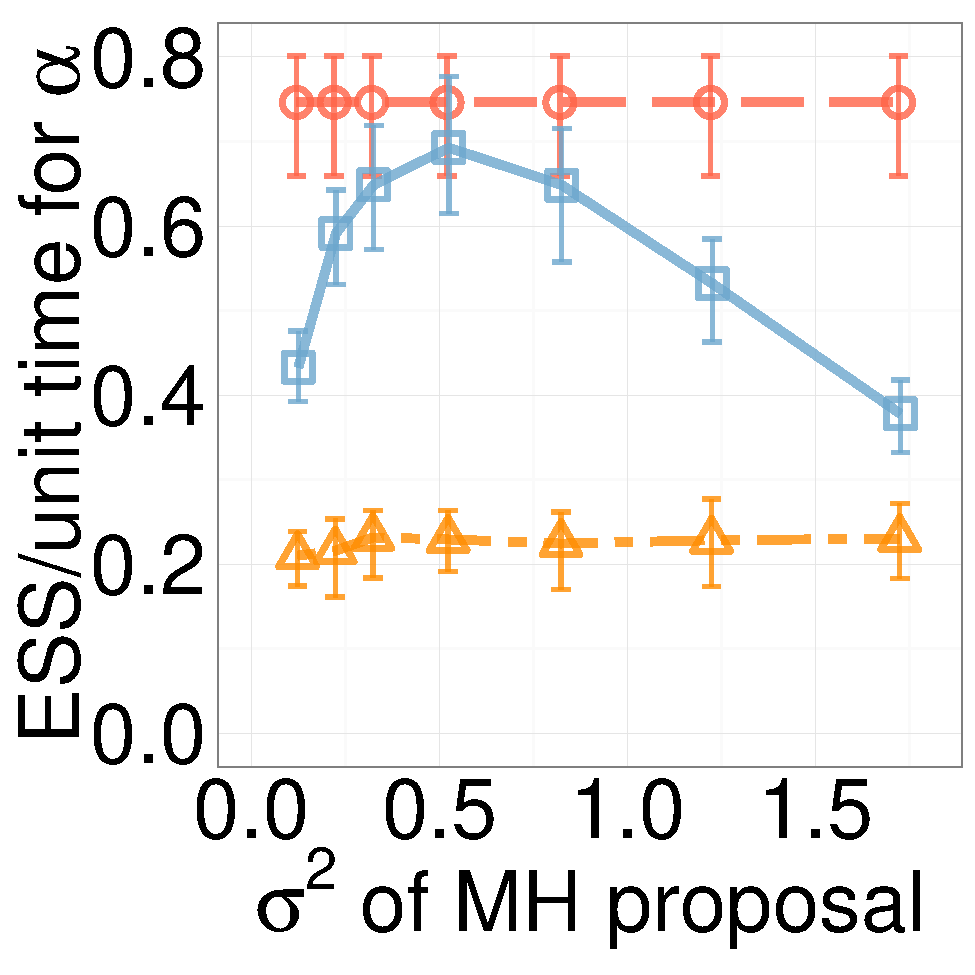
\includegraphics [width=0.49\textwidth, angle=0]{figs/new_experiment_figs/q_alpha_dim10_k2.pdf}
    %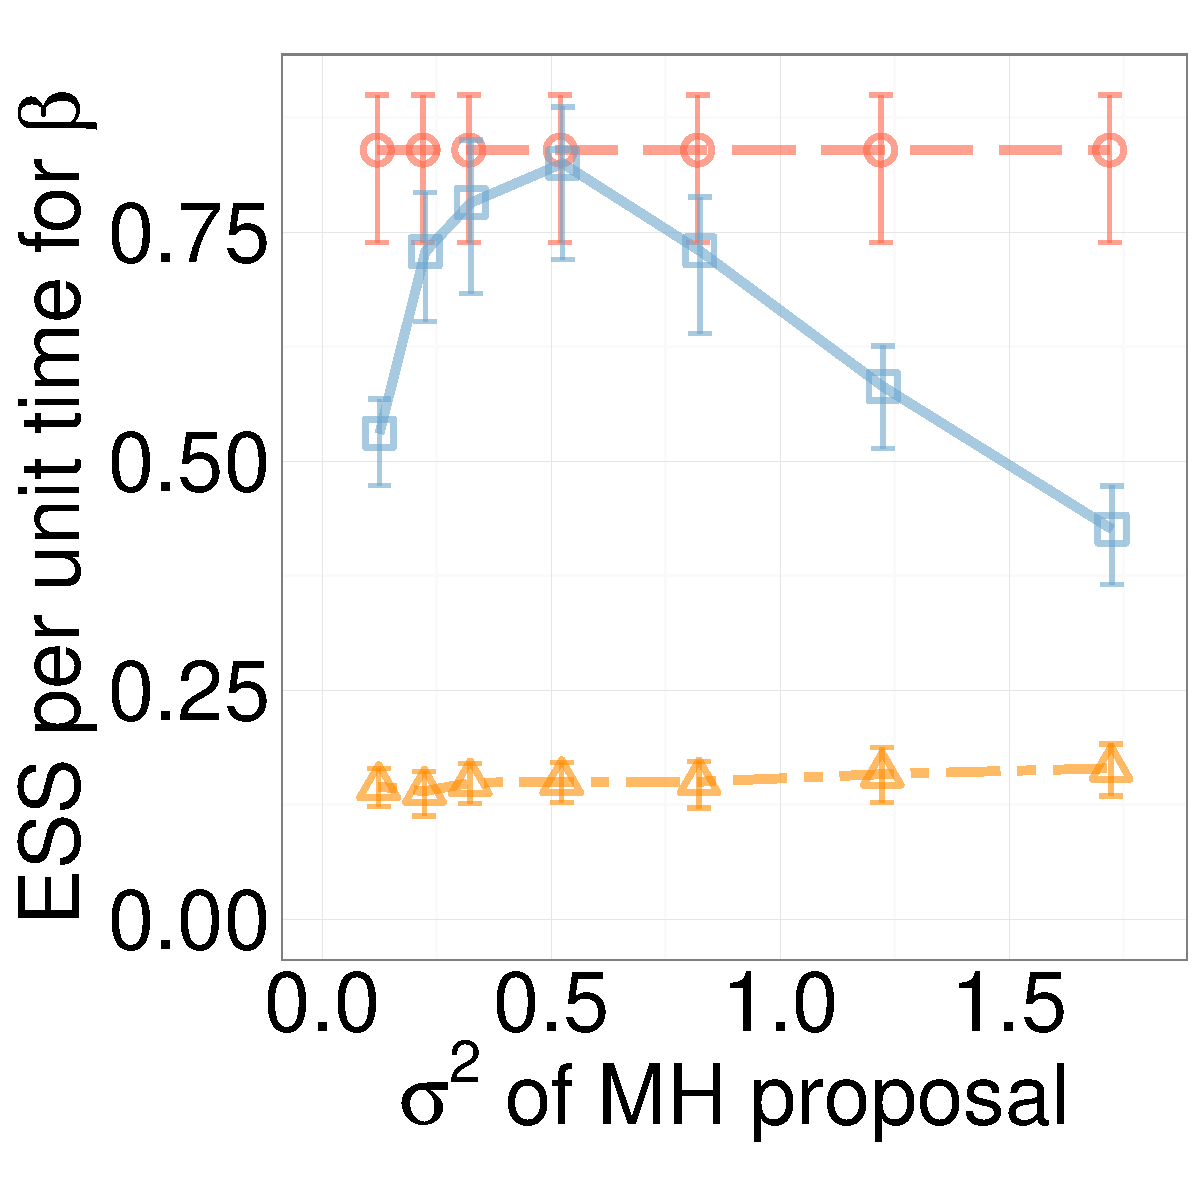
\includegraphics [width=0.49\textwidth, angle=0]{figs/new_experiment_figs/q_beta_dim10_k2.pdf}
    %\vspace{-0.1 in}
  %\end{minipage}
  %\begin{minipage}[!hp]{0.3\linewidth}
   % \caption{ESS/sec for the immigration model, the top row being dimension 3, and the bottom,
     % dimension 10. The left column is for $\alpha$, and the 
    %right is for $\beta$. Red, yellow, and blue curves are the symmetrized MH,
  %\naive\ MH, Gibbs sampling and particle MCMC.}
    % \label{fig:ESS_Q_D10}
  %\end{minipage}
%  \end{figure}
  \begin{figure}[H]
%    \vspace{-.2in}
  \centering
  \begin{minipage}[!hp]{0.24\linewidth}
    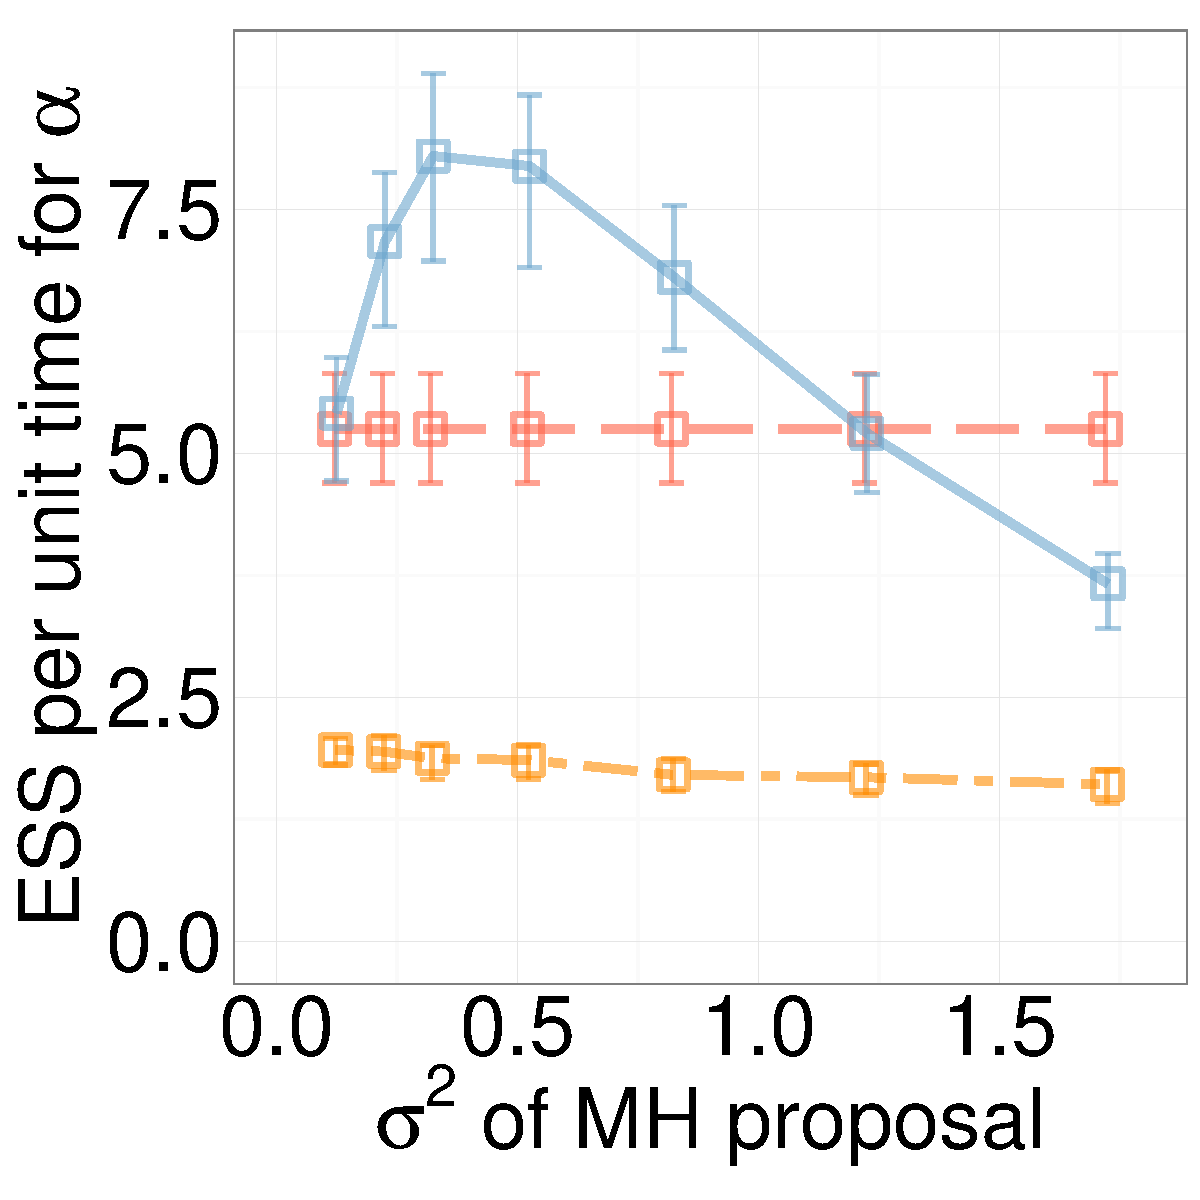
\includegraphics [width=0.99\textwidth, angle=0]{figs/new_experiment_figs/q_alpha_dim3_k2.pdf}
\end{minipage}
  \begin{minipage}[hp]{0.24\linewidth}
  \centering
    \includegraphics [width=0.99\textwidth, angle=0]{figs/new_experiment_figs/q_beta_dim3_k2.pdf}
	\end{minipage}
  \begin{minipage}[hp]{0.24\linewidth}
  \centering
    \includegraphics [width=0.99\textwidth, angle=0]{figs/new_experiment_figs/q_alpha_dim10_k2.pdf}
	\end{minipage}
  \begin{minipage}[hp]{0.24\linewidth}
  \centering
    \includegraphics [width=0.99\textwidth, angle=0]{figs/new_experiment_figs/q_beta_dim10_k2.pdf}
	\end{minipage}
  \centering
  \begin{minipage}[!hp]{0.24\linewidth}
  \centering
    \includegraphics [width=0.99\textwidth, angle=0]{figs/ess/Q_D3alpha_k2.pdf}
\end{minipage}
  \begin{minipage}[hp]{0.24\linewidth}
  \centering
    \includegraphics [width=0.99\textwidth, angle=0]{figs/ess/Q_D3beta_k2.pdf}
	\end{minipage}
  \begin{minipage}[hp]{0.24\linewidth}
  \centering
    \includegraphics [width=0.99\textwidth, angle=0]{figs/ess/Q_D10alpha_k2.pdf}
	\end{minipage}
  \begin{minipage}[hp]{0.24\linewidth}
  \centering
    \includegraphics [width=0.99\textwidth, angle=0]{figs/ess/Q_D10beta_k2.pdf}
	\end{minipage}
     %\label{fig:ESS_Q_notpersec}
%  \begin{minipage}[!hp]{0.3\linewidth}
    \caption{ESS/sec (top row) and raw ESS per 1000 samples (bottom row) for the immigration model. The left two columns are $\alpha$ and $\beta$ for 3 states, and the right two, for 10 states.
    Squares, triangles and circles are symmetrized MH, \naive\ MH, and Gibbs algorithm. }
     \label{fig:ESS_Q_D10}
%  \end{minipage}
  \end{figure}

  \begin{figure}[H]
  \centering
  \begin{minipage}[!hp]{0.24\linewidth}
  \centering
    \includegraphics [width=0.99\textwidth, angle=0]{figs/new_whole_exp_figs/mh_q_alpha_dim3.pdf}
\end{minipage}
  \begin{minipage}[hp]{0.24\linewidth}
  \centering
    \includegraphics [width=0.99\textwidth, angle=0]{figs/new_whole_exp_figs/mh_q_beta_dim3.pdf}
	\end{minipage}
  \begin{minipage}[hp]{0.24\linewidth}
  \centering
    \includegraphics [width=0.99\textwidth, angle=0]{figs/new_whole_exp_figs/mh_q_alpha_dim10.pdf}
	\end{minipage}
  \begin{minipage}[hp]{0.24\linewidth}
  \centering
    \includegraphics [width=0.99\textwidth, angle=0]{figs/new_whole_exp_figs/mh_q_beta_dim10.pdf}
	\end{minipage}
    \caption{ESS/sec for symmetrized MH for the immigration model for different settings of $\Omega(\theta,\vartheta)$. The left two columns are for $\alpha$ and $\beta$ with states, and the right two, with 10. 
    Squares, circles and trianges correspond to $\Omega(\theta,\vartheta)$ set to $(\max_s A_s(\theta) + \max_s A_s(\vartheta))$, $\max(\max_s A_s(\theta), \max_s A_s(\vartheta))$ and  $1.5(\max_s A_s(\theta) + \max_s A_s(\vartheta))$.
  }
    \label{fig:mhESS_Q}
  \end{figure}


Next, we consider an M/M/N/N queue~\citep{gross2011fundamentals}. 
The state space of this stochastic process is $\{0, 1, 2, 3, \cdots, N - 1\}$ giving the number of customers/jobs/individuals in a system/population. 
Arrivals follow a rate-$\alpha$ Poisson process, moving the process from state 
$i$ to $i+1$ for $i<N$. The system has a capacity of $N$, so any arrivals when 
the current state is $N$ are discarded.  Service times or deaths are 
exponentially distributed, with a rate that is now state-dependent:
the system moves from $i$ to $i - 1$ with rate $i\beta$. 
%There are $N$ servers, which serve from the front of the queue. 
%If there are less than $N$ jobs, some of the servers will be idle. 
%Only $N$ customers can queue at any one time. 
%Any further arrivals to the queue are considered ''lost''. 

% \begin{figure}
% \centering
% \begin{minipage}[hp]{0.6\linewidth}%0.45
% \centering
%   \includegraphics [width=1\textwidth, angle=0]{figs/queue_model.pdf}%0.70
%     \end{minipage}
%   \caption{queuing model}
%   \label{q_model}
% \end{figure}



We follow the same setup as the first experiment:
for $(\alpha_0,\alpha_1,\beta_0,\beta_1)$ equal to $(3,2,5,2)$,
we place Gamma$(\alpha_0,\alpha_1)$, and Gamma$(\beta_0, \beta_1)$ priors on $\alpha$, $\beta$. 
These prior distributions are used to sample transition matrices $A$, which, along with a uniform distribution over initial states, are used to generate MJP trajectories. 
We observe these at integer-valued times according to a Gaussian likelihood.
We consider three settings: $3, 5$ and $10$ states, with results from $5$ steps included in the appendix. 

  %\subsection{Experiments}
Figure~\ref{fig:ESS_Q_D10} plots the ESS per unit time (top row) as well as raw ESS values (bottom row) for the parameters $\alpha$ and $\beta$, again as we change the variance of the proposal kernel. 
The left two columns show these for $\alpha$ and $\beta$ for the MJP state-space having size $3$, while the right two columns show these for size $10$.
  %Colors and types are the same as the previous experiment.
Our symmetrized  MH algorithm does best for dimensions $3$ and $5$ (shown in the appendix), although now Gibbs sampling performs best for dimensionality $10$ (although there is no significant different between the best proposal variance for our sampler and the Gibbs sampler).
The Gibbs sampler performs so well partly because the conditionals over $\alpha$ and $\beta$ are conjugate, following simple Gamma distributions. Also, unlike the earlier problem, the rate matrix is tri-diagonal, and governed by two parameters, so that path-parameter coupling is now milder.
% Figure~\ref{fig:hist} shows posterior distributions for 
% $P(\theta | X)$(red), $P(\theta | S, T, X)$(green), $P(\theta | W, X)$(blue). 
% We run $10000$ iterations. The first $5000$ are treated as burn in period. 
% We fix $V_{5000}, W_{5000}$ and then sample $\theta$ from 
% $P(\theta | V_{5000}, W_{5000}, X)$ and sample $\theta$ from 
% $P(\theta | W_{5000}, X)$. We keep updating $S$ and $T$ for sampling from 
% $P(\theta | X)$. We sample another $5000$ $\theta$s to draw the histograms. 
% We can find that $P(\theta | S, T, X)$ and $P(\theta | W, X)$ are both very 
% concentrated which implies the coupling.
% \begin{figure}%[b]
% \begin{minipage}[hp]{0.45\linewidth}
% \centering
%   \includegraphics [width=0.90\textwidth, angle=0]{figs/dist_alpha.pdf}
%   \vspace{-0 in}
% \end{minipage}
% \begin{minipage}[!hp]{0.45\linewidth}
% \centering
%   \includegraphics [width=0.90\textwidth, angle=0]{figs/dist_beta.pdf}
%   \vspace{-0 in}
% \end{minipage}
%   \caption{density.The left is for $\alpha$, and the right is for $\beta$.}
%    \label{fig:dist}
% \end{figure}
% $w(t) = w_i, \; t \in [\l_i, l_{i + 1}), i = 1,2,3,..., K$.
%\noindent Assume: $S = [S_0,S_1, ...,S_N] \;, T = [t_0(t_{start}), t_1,...,t_N, 
%t_{N+1}(t_{end})]$, and y as observations.\\
%Now, let's consider a immigration model as follows. State space is 
% $\{0, 1, 2, ..., N - 1\}$, representing the total population. 
% We already know the conditional density(given $\alpha,\; \beta$) of a MJP trajectory $(s_0, S, T)$ in time interval $[t_{start}, t_{end}]$, with $S=(s_1, s_2,..., s_k)$, $T=(t_1, t_2,..., t_k)$. 
% $$f(s_0,S,T| \alpha, \beta) = \prod_{i=0}^{k-1} A_{s_i, s_{i+1}}(t_i) \exp(\sum_{i=0}^{k} A_{s_i}(t_i)(t_{i+1} - t_{i})), $$
% where $t_0 = t_{start}$, $t_{k+1} = t_{end}.$\\
% Let's denote some notations here.\\
% $$U(s_0, S, T):= \sum_{i=0}^{k-1} \mathbb{I}_{\{s_{i+1} - s_i = 1\}}.$$
% $$D(s_0, S, T):= \sum_{i=0}^{k-1} \mathbb{I}_{\{s_{i+1} - s_i = -1\}}.$$
% Call them U and D for short.
% Let's denote the total time when the trajectory state stays at state i as $\tau_i$, i.e. $\tau_i = \sum_{j=0}^{k} (t_{j+1} -t_j)\mathbb{I}_{\{s_j = i\}}$, then $\sum_{i=0}^k (t_{i+1} - t_i)s_i = \sum_{i=0}^N \tau_ii.$\\

% $$f(s_0,S,T| \alpha, \beta) \propto \exp(\sum_{r = 0}^{K}-w_r\alpha(l_{r + 1} - l_{r}- \tau_N^r) )\alpha^U \cdot  \exp(-\int_{t_s}^{t_{e}}(S(t)w(t)\beta)  \beta^D$$\\
% If we assume the prior of $\alpha$, and $\beta$ are $Gamma(\mu,\lambda)$, $Gamma(\omega, \theta)$, which are independent with each other. \\
% $$p(\alpha) = \frac{\lambda^\mu}{\Gamma(\mu)}\alpha^{\mu -1}e^{-\lambda \alpha}. $$
% $$p(\beta) = \frac{\theta^\omega}{\Gamma(\omega)}\beta^{\omega -1}e^{-\theta \beta}. $$
% Then we can get the posterior distribution $$f(\alpha, \beta | s_0,S,T)$$ as follows.
% $$ f(\alpha, \beta | s_0,S,T) \propto \exp(-(\lambda +\sum_{r = 0}^{K}w_r\alpha(l_{r + 1} - l_{r}- \tau_N^r))\alpha) \alpha^{\mu + U -1} \cdot \exp(-(\int_{t_{s}}^{t_{e}}(S(t)w(t) + \theta)\beta) \beta^{\omega+ D -1}.$$
% It means that the posterior distributions of $\alpha$, $\beta$ are still independent. \\
% $\alpha | s_0,S,T$ is following $Gamma(\mu+ U,\lambda +\sum_{r = 0}^{K}w_r\alpha(l_{r + 1} - l_{r}- \tau_N^r)  )$\\
% $\beta | s_0,S,T$ is following $Gamma(\omega+ D,\int_{t_s}^{t_{e}}(S(t)w(t) + \theta)$.\\
% Such immigration models have perfectly conjugate posterior distributions when we assign $\gamma$ priors to $\alpha$ and $\beta$. We apply our Metropolis Hasting algorithms on such models to compare the performance with the performance of Gibbs Sampling algorithm.

%\subsection{Experiments}


  \begin{figure}%[b]
  \centering
  \begin{minipage}[hp]{0.35\linewidth}
  \centering
    \vspace{-0 in}
    \includegraphics [width=0.98\textwidth, angle=0]{figs/dist_beta_50.pdf}
  \end{minipage}
  \begin{minipage}[hp]{0.64\linewidth}
%   \vspace{-0.3 in}
  \caption{Prior distribution of an MJP parameter (the wide red density), with two conditional distributions. 
    Narrow dotted-green is the density conditioned on both the observations as well as a simulated MJP posterior. 
    The wider dashed-blue curve is density of interest: the marginal distribution of the parameters conditioned on observations. 
	\boqian{The time interval is $[0, 50]$.}
}
     \label{fig:hist_50}
  \end{minipage}
%   \vspace{-0.6 in}
  \end{figure}

  \begin{figure}%[b]
  \centering
  \begin{minipage}[hp]{0.35\linewidth}
  \centering
    \vspace{-0 in}
    \includegraphics [width=0.98\textwidth, angle=0]{figs/dist_beta_100.pdf}
  \end{minipage}
  \begin{minipage}[hp]{0.64\linewidth}
%   \vspace{-0.3 in}
  \caption{Prior distribution of an MJP parameter (the wide red density), with two conditional distributions. 
    Narrow dotted-green is the density conditioned on both the observations as well as a simulated MJP posterior. 
    The wider dashed-blue curve is density of interest: the marginal distribution of the parameters conditioned on observations. 
	\boqian{The time interval is $[0, 100]$.}
}
     \label{fig:hist_50}
  \end{minipage}
%   \vspace{-0.6 in}
  \end{figure}

%  \begin{figure}%[b]
%  \centering
 %\begin{minipage}[!hp]{0.68\linewidth}
  %\centering
   % \includegraphics [width=0.49\textwidth, angle=0]{figs/new_experiment_figs/cq_alpha_dim3_k2.pdf}
    %\includegraphics [width=0.49\textwidth, angle=0]{figs/new_experiment_figs/cq_beta_dim3_k2.pdf}
  %\centering
   % \includegraphics [width=0.49\textwidth, angle=0]{figs/new_experiment_figs/cq_alpha_dim10_k2.pdf}
    %\includegraphics [width=0.49\textwidth, angle=0]{figs/new_experiment_figs/cq_beta_dim10_k2.pdf}
    %\vspace{-.3 in}

%  \end{minipage}
 % \begin{minipage}[!hp]{0.01\linewidth}
  %\end{minipage}
 % \begin{minipage}[!hp]{0.3\linewidth}
%    \vspace{-.3in}
%    \caption{ESS/sec for the time-inhomogeneous immigration model, the top row 
  %    being dimension 3, and the bottom,
    %  dimension 10. The left column is for $\alpha$, and the 
    %right is for $\beta$. Red, yellow and blue curves are the symmetrized MH,
  %\naive\ MH, and Gibbs algorithm.}
    % \label{fig:ESS_pc_10}
  %\end{minipage}
 % \end{figure}

  \begin{figure}[H]
%    \vspace{-.2in}
  \centering
  \begin{minipage}[!hp]{0.24\linewidth}
    \includegraphics [width=0.99\textwidth, angle=0]{figs/new_experiment_figs/cq_alpha_dim3_k2.pdf}
\end{minipage}
  \begin{minipage}[hp]{0.24\linewidth}
  \centering
    \includegraphics [width=0.99\textwidth, angle=0]{figs/new_experiment_figs/cq_beta_dim3_k2.pdf}
	\end{minipage}
  \begin{minipage}[hp]{0.24\linewidth}
  \centering
    \includegraphics [width=0.99\textwidth, angle=0]{figs/new_experiment_figs/cq_alpha_dim10_k2.pdf}
	\end{minipage}
  \begin{minipage}[hp]{0.24\linewidth}
  \centering
    \includegraphics [width=0.99\textwidth, angle=0]{figs/new_experiment_figs/cq_beta_dim10_k2.pdf}
	\end{minipage}
%  \begin{minipage}[!hp]{0.3\linewidth}
  \centering
  \begin{minipage}[!hp]{0.24\linewidth}
  \centering
    \includegraphics [width=0.99\textwidth, angle=0]{figs/ess/QC_D3alpha_k2.pdf}
\end{minipage}
  \begin{minipage}[hp]{0.24\linewidth}
  \centering
    \includegraphics [width=0.99\textwidth, angle=0]{figs/ess/QC_D3beta_k2.pdf}
	\end{minipage}
  \begin{minipage}[hp]{0.24\linewidth}
  \centering
    \includegraphics [width=0.99\textwidth, angle=0]{figs/ess/QC_D10alpha_k2.pdf}
	\end{minipage}
  \begin{minipage}[hp]{0.24\linewidth}
  \centering
    \includegraphics [width=0.99\textwidth, angle=0]{figs/ess/QC_D10beta_k2.pdf}
	\end{minipage}
%     \label{fig:ESS_CQ_notpersec}
    \caption{ESS/sec (top row) and raw ESS per 1000 samples (bottom row) for the time-inhomogeneous immigration model. The left columns are $\alpha$ and $\beta$ for 3 states, and the right two for 10. {Blue squares, yellow triangles and red circles} are the symmetrized MH, \naive\ MH, and Gibbs algorithm. }
     \label{fig:ESS_pc_10}
%  \end{minipage}
  \end{figure}


  \begin{figure}[H]
  \centering
  \begin{minipage}[!hp]{0.24\linewidth}
  \centering
    \includegraphics [width=0.99\textwidth, angle=0]{figs/new_whole_exp_figs/mh_cq_alpha_dim3.pdf}
\end{minipage}
  \begin{minipage}[hp]{0.24\linewidth}
  \centering
    \includegraphics [width=0.99\textwidth, angle=0]{figs/new_whole_exp_figs/mh_cq_beta_dim3.pdf}
	\end{minipage}
  \begin{minipage}[hp]{0.24\linewidth}
  \centering
    \includegraphics [width=0.99\textwidth, angle=0]{figs/new_whole_exp_figs/mh_cq_alpha_dim10.pdf}
	\end{minipage}
  \begin{minipage}[hp]{0.24\linewidth}
  \centering
    \includegraphics [width=0.99\textwidth, angle=0]{figs/new_whole_exp_figs/mh_cq_beta_dim10.pdf}
	\end{minipage}
    \caption{ESS/sec for symmetrized MH for the time-inhomogeneous immigration model for different settings of $\Omega(\theta,\vartheta)$. The left two columns are $\alpha$ and $\beta$ for 3 states, and the right two for 10. 
    Squares, circles and trianges correspond to $\Omega(\theta,\vartheta)$ set to $(\max_s A_s(\theta) + \max_s A_s(\vartheta))$, $\max(\max_s A_s(\theta), \max_s A_s(\vartheta))$ and  $1.5(\max_s A_s(\theta) + \max_s A_s(\vartheta))$.}
     \label{fig:mhESS_CQ}
  \end{figure}



\noindent \textbf{A time-inhomogeneous immigration model:}
We extend the previous model to incorporate a known time-inhomogeneity. 
The arrival and death rates are now no longer constant, and are instead given by
 %$$A_i(t) =: A_{i,i}(t) = -(\alpha + i\beta)w(t), \; \; i =0,1,...,N$$ 
$A_{i, i+1}(t) = \alpha w(t) \ (i =0,1,\cdots,N-1)$ respectively.
While it is not difficult to work with sophisticated choices of $w(t)$, we limit ourselves to a simple piecewise-constant $w(t) = \left\lfloor \frac{t}{5} \right\rfloor$. 
Even such a simple change in the original model can dramatically affect the performance of the Gibbs sampler. 

 The top row of figure~\ref{fig:ESS_pc_10} plots the ESS per unit time for the parameters $\alpha$ (left) and $\beta$ (right) for this model with capacity $3$.  
 Now, the symmetrized MH algorithm is significantly more efficient, comfortably outperforming all samplers (including the Gibbs 
 sampler) over a wide range of settings. %The Gibbs sampler slightly outperforms
 %the simple MH sampler, while particle MCMC is significantly worse (we have
% not included it).  
 Figure~\ref{fig:ESS_pc_10} shows performance for dimension $10$, once again the symmetrized MH-algorithm performans best over a range of settings of the proposal variance. We note that increasing the
 dimensionality of the state space results in a more concentrated posterior, shifting the optimal setting of the proposal variance to smaller values.
 \vinayak{explain new figure}

  \subsection{Chi site data for Escherichia coli}~
  We consider a dataset recording positions of a particular DNA motif 
  on the {\em E.\ coli} genome. 
  These motifs consist of eight base pairs GCTGGTGG, and are called Chi sites~\citep{FearnSher2006}.
  The rates of occurence of Chi sites provide information about genome 
  segmentation, allowing the identification of regions with high 
  mutation or recombination rates.
  %strands which are the inner and outer rings. The molecular mechanisms 
  %of DNA replication differ between the two half-strands and they are 
  %termed leading and lagging. The E. coli genome is 4639675 bases long and 
  %each half is 2319.838 kilobases long. 
  Following~\cite{FearnSher2006}, we use this data to infer a two-state piecewise-constant segmentation of the DNA strand. 
  We focus on Chi sites along the inner (lagging) strand of the {\em E.\ coli} genome.  
  We place a MJP prior over this segmentation, and indexing position along the 
  strand with $t$, we write this as $S(t), t \in [0,2319.838]$. 
  To each state $s \in \{1,2\}$, we assign a rate $\lambda_s$, which together with $S(t)$, defines a piecewise-constant rate function $\lambda_{S(t)}$. 
  We model the Chi-site positions as drawn from a Poisson process with rate 
  $\lambda_{S(t)}$, resulting in a {Markov-modulated Poisson process}~\citep{scottmmpp03} (see also section~\ref{sec:bayes_model}). 
  MJP transitions from state $1$ to state $2$ have rate $\alpha$ while transitions from state $2$ to state $1$ have rate $\beta$. 
  We place gamma priors on the four model parameters; specifically, we use Gamma$(2,2)$, Gamma$(2,3)$, Gamma$(3,2)$, Gamma$(1,2)$ for $\alpha$, $\beta$, $\lambda_1$, $\lambda_2$ respectively.


  We use this setup to evaluate our symmetrized MH sampler along with Gibbs sampling (other algorithms perform much worse, and we do not include them). 
  For our MH proposal distribution, we first run {2000} iterations of Gibbs sampling to estimate the posterior covariance of the vector $\theta = (\alpha,\beta,\lambda_1,\lambda_2)$, call this $\Sigma_\theta$. 
  Our MH proposal distribution is then $q(\nu|\theta) = N(\nu|\theta, \sigma^2\Sigma_\theta)$ for different settings of $\sigma^2$ (the typical choice is $\sigma^2 = 1$),
 % \boqian{(we might want to change $\kappa$ here, because we use $\kappa$ in the beginning of the section for different meaning.)} \boqian{,
where we set $\Omega(\theta, \vartheta) = \max_s A_s(\theta) + \max_s A_s(\vartheta)$. 

  Figure~\ref{fig:TRACE_ECOLI} shows trace and autocorrelation plots for the parameter $\alpha$ produced by the Gibbs sampler (left) and our proposed sampler with $\kappa$ set to $1$.
  We see that this is a fairly hard MCMC sampling problem, however our sampler clearly outperforms Gibbs, which mixes very poorly.
  Both posterior distribution agreed with each other though, with a two sample-Kolmogorov Smirnov test returning a p-value of $ 0.1641$. 
  \begin{figure}[H]
%    \vspace{-.2in}
  \centering
%  \begin{minipage}[!hp]{0.99\linewidth}
 % \centering
  \begin{minipage}[!hp]{0.99\linewidth}
    \includegraphics [width=0.24\textwidth, angle=0]{figs/ecoli_ks/ecoli_alphatraceGBS_31_3_0_.pdf}
    \includegraphics [width=0.24\textwidth, angle=0]{figs/ecoli_ks/ecoli_alphagbsacf_31_3_0_.pdf}
    \includegraphics [width=0.24\textwidth, angle=0]{figs/ecoli_ks/ecoli_alphatraceMH_31_3_0_.pdf}
    \includegraphics [width=0.24\textwidth, angle=0]{figs/ecoli_ks/ecoli_alphamhacf_31_3_0_.pdf}
  \end{minipage}

%  \end{minipage}
%  \begin{minipage}[!hp]{0.99\linewidth}
    \caption{Trace and autocorrelation plots of posterior samples for $\alpha$ for the E.\ Coli data. The left two plots are the Gibbs sampler and the right two are the symmetrized MH. }
     \label{fig:TRACE_ECOLI}
%  \end{minipage}
  \end{figure}
  Figure~\ref{fig:ECOLI} shows the ESS/s for different settings of $\kappa$, for parameters $(\alpha, \lambda_1)$. 
  Both parameters have very similar results, and as suggested by the earlier figure, we see that for the typical setting of $\kappa=1$, our sampler ourperforms the Gibbs sampler. 
  In this problem though, Gibbs sampling does outperform our method for large or small $\kappa$. 
  This is because a) large or small $\kappa$ mean the proposal variance is too large or too small, and b) the Gibbs conditionals over the parameters are conjugate for this model. 
  We expect the improvements our method offers to be more robust to the proposal distribution for more complex models without such conditional conjugacy.
  \begin{figure}[H]
%    \vspace{-.2in}
  \centering
%  \begin{minipage}[!hp]{.32\linewidth}
%    \caption{ESS/sec for $(\alpha,\lambda_1)$ for the E.\ Coli data. The circles (in blue) are our 
%      proposed sampler as we vary the variance of the proposal distribution. 
 %     The straight line is the Gibbs sampler. }
  %   \label{fig:ECOLI}
%  \end{minipage}
%  \begin{minipage}[!hp]{.65\linewidth} 
  \begin{minipage}[!hp]{.68\linewidth}
    %\includegraphics [width=0.48\textwidth, angle=0]{figs/ECOLI_alpha.pdf}
    %\includegraphics [width=0.48\textwidth, angle=0]{figs/ECOLI_l1.pdf}
	\includegraphics [width=0.48\textwidth, angle=0]{figs/new_experiment_figs/ecoli_alpha.pdf}
	\includegraphics [width=0.48\textwidth, angle=0]{figs/new_experiment_figs/ecoli_l1.pdf}
			%    \vspace{-.81 in}
 			%	   \includegraphics [width=0.24\textwidth, angle=0]{figs/ECOLI_beta.pdf}
 			%  \includegraphics [width=0.24\textwidth, angle=0]{figs/ECOLI_l2.pdf}
			%    \vspace{-.2in}
  \end{minipage}  
  \begin{minipage}[!hp]{.01\linewidth}
  \end{minipage}
  \begin{minipage}[!hp]{.3\linewidth}
    \caption{ESS/sec for $(\alpha,\lambda_1)$ for the E.\ Coli data. The circles (in blue) are our 
      proposed sampler as we vary the variance of the proposal distribution. 
      The straight line is Gibbs. }
     \label{fig:ECOLI}
  \end{minipage}  

%   \vspace{-.3in}
  \end{figure}


% \begin{figure}[H]
% \centering
% \begin{minipage}[!hp]{0.99\linewidth}
%   \includegraphics [width=0.24\textwidth, angle=0]{figs/ecoli_ks/ecoli_l1traceGBS_31_3_0_.pdf}
%   \includegraphics [width=0.24\textwidth, angle=0]{figs/ecoli_ks/ecoli_l1traceMH_31_3_0_.pdf}
%   \includegraphics [width=0.24\textwidth, angle=0]{figs/ecoli_ks/ecoli_l1gbsacf_31_3_0_.pdf}
%   \includegraphics [width=0.24\textwidth, angle=0]{figs/ecoli_ks/ecoli_l1mhacf_31_3_0_.pdf}
% \end{minipage}
%   \caption{The left is histogram for the posterior samples($\lambda_1$) for the E.\ Coli data.The red and blue curves are the Gibbs and symmetrized MH. The p value of the two sample-Kolmogorov Smirnov test is $ 0.4658$. The middle and the right are trace plots for the posterior samples for the E.\ Coli data, the middle is for Gibbs and the right is for symmetrized MH}
%    \label{fig:TRACE_ECOLI_l1}
% \end{figure}

% \begin{figure}%[b]
% \centering
% \begin{minipage}[!hp]{0.99\linewidth}
% \centering
%   \includegraphics [width=0.25\textwidth, angle=0]{figs/ECOLI_alpha.pdf}
%   \includegraphics [width=0.25\textwidth, angle=0]{figs/ECOLI_l1.pdf}
%  %   \includegraphics [width=0.24\textwidth, angle=0]{figs/ECOLI_beta.pdf}
%  %  \includegraphics [width=0.24\textwidth, angle=0]{figs/ECOLI_l2.pdf}
% %  \vspace{-.5in}
% \end{minipage}
%   \vspace{-.2in}
%   \caption{ESS/sec for the EColi data.}
%    \label{fig:ECOLI}
% \end{figure}

